\documentclass[11pt]{article}
\usepackage{amsmath,amssymb,amsthm}
\usepackage{mathtools}
\usepackage{geometry}
\usepackage[hypertexnames=false]{hyperref}
\usepackage{enumitem}
\usepackage{tikz}
\usepackage{float}
\usetikzlibrary{calc}
\usetikzlibrary{positioning}
\usetikzlibrary{decorations.pathreplacing}
\geometry{margin=1in}

\newtheorem{theorem}{Theorem}[section]
\newtheorem{definition}{Definition}[section]
\newtheorem{lemma}{Lemma}[section]
\newtheorem{proposition}{Proposition}[section]
\newtheorem{corollary}{Corollary}[section]
\newtheorem{remark}{Remark}[section]
\newcommand{\mainref}[1]{\ref{#1}}

\title{The Catalan Light Cone:\\
Dyck Paths as a Discrete Substrate for Causal Geometry, Quantum Amplitudes, and Computation}
\author{Paul Fernandez}
\date{}

\begin{document}
\maketitle

\begin{abstract}
\noindent
We study the Catalan family of structures (Dyck paths, full binary trees, and
balanced parentheses) as a single discrete space of admissible histories with
multiple equivalent ``coordinate systems.'' The Dyck constraint
induces a natural causal prefix order, and organizing histories by semilength
(tier) and lateral spread yields a discrete cone whose extremal configurations reproduce a
light-cone--like causal envelope (terminology is mnemonic; no discrete Lorentz
symmetry is claimed).

Classical results on conditioned random walks imply that, under diffusive
scaling, Dyck ensembles converge to Brownian excursions. This provides a
continuum comparison. The base diffusion generator is the heat operator on the
half-line, with the Dyck conditioning encoded via a Doob transform / Bessel-bridge
representation. Phase weighting admits a standard Feynman--Kac interpretation.
Under analytic continuation one obtains the free Schr\"odinger equation.

The same Catalan shapes also serve as unlabeled application skeletons for
$\lambda$-calculus and SKI terms (after choosing a standard finite encoding of
symbols). Under this reading, causal extension aligns with functional
application while local collapse aligns with computational reduction. We also
present a minimal Catalan amplitude model: given an observable/coarse-graining
$f$ and a phase functional (e.g.\ Dyck area), coherent summation over
the preimages $f^{-1}(x)$ produces interference under Born-style squaring.

Complex phases and Born-style readout are part of the amplitude model. Extending
the dynamics to include interactions, constants, and selection rules remains open.
\end{abstract}

\section{Introduction}
Discrete approaches to fundamental physics suggest that continuum
spacetime and quantum dynamics may emerge from deeper combinatorial structure.
Examples include causal sets \cite{bombelli87}, discrete random surfaces and
Causal Dynamical Triangulations (CDT) \cite{ambjorn01,ambjorn12}, spin
networks and loop quantum gravity \cite{rovelli04}, tensor networks
\cite{orus14}, and rewriting systems inspired by $\lambda$-calculus and
combinatory logic.

Typically, however, these models require multiple independent ingredients: a
relation or graph for causal structure, an algebra for computation, and
additional rules for quantum propagation. This work explores a more economical
possibility: that a \emph{single} recursive structure simultaneously supports
all three.

The focus is the \emph{Catalan substrate}, the family of structures counted by
the Catalan numbers \cite{stanley-catalan}, including Dyck paths, full binary
trees, and balanced parentheses. These objects are usually studied
in enumerative combinatorics, probability theory, and theoretical computer
science. Here they are treated instead as a space of \emph{admissible
histories} generated by a minimal growth constraint.

\paragraph{One object, three coordinate systems.}
We will move freely between three canonically bijective Catalan families:
\begin{itemize}
  \item Dyck paths (a constrained nearest-neighbour walk),
  \item full binary trees (recursive branching structure),
  \item parentheses/pairs encodings (a linear trace of the same tree).
\end{itemize}
Switching between these views is not a simulation; it is a change of
representation of the same underlying object. Each view foregrounds different
structure: Dyck paths make causal order and scaling limits transparent; trees
make locality and computation transparent; and pairs encodings make uniform
syntax convenient.

\paragraph{Pairs-only locality discipline.}
Throughout, the Catalan object itself is the only combinatorial configuration
(state). Concretely:
\begin{itemize}
	\item Apart from an optional finite leaf-label encoding when representing
		programs, we do not attach independent labels, fields, or global degrees of
		freedom to the substrate.
	\item Observables, weights, phases, and amplitudes are functions of the Catalan
		object (or of local update events), not additional state variables.
	\item Single-step dynamics are specified by local subtree rewrites (finite
		patterns).
	\item Global-looking weights or statistics are introduced together with explicit
		pair-local decompositions, either as step-additive functionals along Dyck growth
		or as recursive folds on the pairing tree (see
		Proposition~\ref{prop:phase-classification} and
		Lemma~\ref{lem:additive-gauge-invariant}).
\end{itemize}

\paragraph{Contributions and scope.}
The paper isolates a common structural core shared by three domains:
\begin{enumerate}[label=(\roman*)]
	\item \textbf{Causal geometry:} the prefix order on Dyck prefixes induces a
		discrete causal structure and a cone-shaped envelope with sharp extremals.
		\item \textbf{Continuum comparison:} classical conditioned-walk results yield a
			diffusion limit (Brownian excursion; the half-line heat operator as a base
			diffusion generator with the conditioning encoded by a Doob transform), and an
			analytic-continuation bridge to the free Schr\"odinger equation
			\cite{le-gall05,janson07,feynman-hibbs65,kac49}.
		\item \textbf{Computation:} Catalan tree shapes provide unlabeled application
			skeletons for standard Turing-complete functional calculi (after choosing a
			finite encoding of symbols), and local reductions remain internal to the same
			family \cite{church33,CurryFeys1958,barendregt84}.
		\item \textbf{Amplitudes:} we define a minimal Catalan amplitude model in which
			a coarse-graining (observable) and a phase functional determine a coherent sum
			over indistinguishable histories, producing interference under Born-style squaring.
\end{enumerate}

\paragraph{Model layers and scope (read-first).}
This paper separates \emph{kinematics} from \emph{dynamical overlays}:
\begin{itemize}
	\item \textbf{Kinematics:} the Catalan substrate and its causal prefix order.
		We use the term ``Catalan light cone'' for the cone-shaped growth envelope of
		Dyck histories in the $(n,b)$ diagram; no discrete Lorentz symmetry is assumed.
	\item \textbf{Amplitudes:} a minimal model in which an observable/coarse-graining
		$f$ and an additive phase functional determine complex weights on histories,
		with readout by squared magnitudes after coarse-graining.
	\item \textbf{Computation:} the classical representation of applicative terms by
		binary application trees and local rewrites.
\end{itemize}
The technical goal is to show that each overlay can be expressed by pair-local
operations on the same substrate. Selecting physically preferred dynamics
(interactions, calibration, and selection rules) is left open.

\paragraph{Organization.}
Section~\ref{sec:catalan_cone} establishes the discrete causal geometry of the
Catalan lattice and its cone-shaped growth envelope. Section~\ref{sec:computation}
develops the computational correspondence via binary application trees and pairs
encodings. Section~\ref{sec:amplitudes} introduces a minimal amplitude
construction and the continuum comparison to diffusion and Schr\"odinger
dynamics.%
\footnote{Depending on reader background, Sections~\ref{sec:computation} and
Section~\ref{sec:amplitudes} may be read in either order after the geometric
setup in Section~\ref{sec:catalan_cone}.}
Locality and disjoint-commutation are discussed in Section~\ref{sec:locality}.
	Sections~\ref{sec:discussion}--\ref{sec:conclusion} provide contextual discussion
	and summarize scope and limitations.
	Appendices collect optional coordinate charts (continuum comparison tools) and
	a worked finite example, separate from the main formal development. Additional
	appendices and extended proof sketches appear in later appendices.

\section{The Catalan Light Cone as a Discrete Causal Geometry}
\label{sec:catalan_cone}

\subsection{Dyck paths and growth tiers}
A Dyck path of semilength $n$ is a walk on the integers satisfying
\[
	H_{k+1} = H_k \pm 1, \qquad H_k \ge 0, \qquad H_0 = H_{2n} = 0.
\]
Equivalently, Dyck paths are balanced-parentheses strings or full binary trees
with $n$ internal nodes. The number of such paths is the $n$th Catalan number
\[
	C_n = \frac{1}{n+1}\binom{2n}{n}.
\]
Each up--down pair \(()\) represents a minimal unit of growth. The integer $n$
will be called the \emph{tier} and will be interpreted as a discrete time
parameter.

\subsection{Prefix order and causality}
Let $\mathcal{C}$ denote the set of \emph{Dyck prefixes}: balanced-parentheses
prefixes that never go below height $0$. Define a partial order by extension:
$u\preceq v$ iff $u$ is a prefix of $v$. We interpret this order as a causal
relation: $u\preceq v$ means that $u$ lies in the causal past of $v$, while
prefixes that diverge represent incompatible futures. This prefix order defines
a discrete causal structure:
\begin{itemize}
		\item every node has a unique causal past,
		\item multiple incompatible futures may branch from the same prefix,
		\item cycles are prohibited by construction.
\end{itemize}
		No additional causal axiom is introduced; causality is enforced combinatorially
		by the Dyck constraint.
		Appendix~\ref{appendix:uniqueness} records an axiomatic characterization of this
		collision-free two-move growth structure, and Appendix~\ref{appendix:unfoldings}
		extends the characterization to growth systems with merges via an explicit
		unfolding construction.

\subsection{Extremal configurations: chain and star}
At fixed tier $n$ there are many Dyck paths. Two extremal configurations play a
distinguished role:
\begin{itemize}
	\item the \emph{chain} (or spine)
		\[
			(((\cdots))),
		\]
		fully nested, with maximal depth and minimal spread;
	\item the \emph{star}
		\[
			()()()\cdots(),
		\]
		fully separated, with minimal depth and maximal spread.
\end{itemize}
All other configurations interpolate between these extremes. Together, the set
of Dyck paths at tier $n$ forms a discrete envelope bounded by the chain and
the star.

\begin{remark}[Narayana refinement by peak count]
In addition to coarse parameters such as depth or breadth, there is a canonical
refinement of the tier by the number of \emph{peaks} of a Dyck path (equivalently,
the number of occurrences of the pattern \texttt{()}). The Narayana numbers
$N(n,k)$ count Dyck paths of semilength $n$ with exactly $k$ peaks and admit the
closed form
\[
N(n,k)=\frac{1}{n}\binom{n}{k}\binom{n}{k-1},\qquad 1\le k\le n,
\]
with $\sum_{k=1}^{n} N(n,k)=C_n$ \cite{stanley-catalan}. The chain has one peak
($k=1$) and the star has $n$ peaks ($k=n$). This gives a natural stratification
of the tier into $k$-sectors that interpolate between the two extremes.
\par
The peak count is a local pattern statistic: for $w=w_1\cdots w_{2n}$ define
\[
k(w):=\sum_{j=1}^{2n-1}\mathbf{1}\{(w_j,w_{j+1})=(\texttt{(},\texttt{)})\}.
\]
\end{remark}

\begin{figure}[ht]
			\centering
			\begin{tikzpicture}[scale=1.1]
  % axes
  \draw[->] (0,0) -- (0,4) node[left] {$n$};
  \draw[->] (0,0) -- (4,0) node[below] {$b$};

  % cone boundaries
  \draw[thick] (0,0) -- (3.5,3.5);
  \draw[thick] (0,0) -- (0.8,3.5);

  % discrete layers
  \foreach \y in {1,2,3} {
    \draw[dashed] (0.25*\y,\y) -- (0.85*\y,\y);
  }

  % labels
  \node[left] at (0,3.6) {chain (axis)};
  \node[above right] at (3.5,3.5) {boundary (star)};
  \node at (1.1,2.2) {\small Dyck layer};
\end{tikzpicture}

					\caption{The Catalan light cone.
						Tier $n$ (the number of Dyck units) plays the role of a discrete time
						coordinate, while breadth $b$ measures lateral spread.
						All Dyck configurations at fixed tier lie between the fully nested chain
						(axis extreme) and the fully separated star (boundary extreme).
						Discrete Dyck layers approximate constant-time hypersurfaces, and the bound
					$b \le n$ is enforced combinatorially.}
					\label{fig:catalan-cone}
			\end{figure}
	
	\subsection{Breadth as spatial extent}
	Define the \emph{breadth} $b(w)$ of a Dyck path $w$ to be the size of a
	largest level set in the nesting-depth decomposition of matched pairs:
	\[
		b(w) := \max_{\ell} \{\text{number of matched pairs at nesting depth } \ell\}.
	\]
	Equivalently, $b(w)$ is the maximal number of non-overlapping pairs at a common
	nesting depth. For a Dyck word of tier $n$ there are $n$ matched pairs in total,
	so
	\[
		1 \le b(w) \le n,
	\]
	with $b=1$ for the fully nested chain and $b=n$ for the fully separated star.
			The inequality
			\[
				b \le n
			\]
			is enforced purely by the recursive constraint. We refer to it as a discrete
			light-cone bound by analogy with $|\Delta x| \le \Delta t$ (in units with
			$c=1$); see Remark~\ref{rem:no-lattice-boost} for the scope of this analogy.

	\begin{remark}[Breadth as a recursive fold]
	\label{rem:breadth-fold}
	Although $b(w)$ is a statistic of a completed history, it is computed by a
	recursive fold on the standard Catalan decomposition. For each Dyck word $w$,
	let $L_w(\ell)$ be the number of matched pairs of $w$ at nesting depth $\ell$, so
	$b(w)=\max_{\ell} L_w(\ell)$ and $L_\varepsilon(\ell)=0$ for the empty word. If
	$w=\texttt{(}u\texttt{)}v$ with $u,v$ Dyck words, then
	\[
		L_w(1)=1+L_v(1),
	\qquad
	L_w(\ell+1)=L_u(\ell)+L_v(\ell+1)\quad(\ell\ge 1).
\]
Equivalently, if $w=w_1\cdots w_{2n}$ has height process $(H_k)_{k=0}^{2n}$, then
each opening symbol $w_k=\texttt{(}$ opens a pair at nesting depth $H_k$, so
\[
L_w(\ell)=\sum_{k=1}^{2n}\mathbf{1}\{w_k=\texttt{(},\ H_k=\ell\}.
\]
\end{remark}

	\subsection{Depth--breadth tradeoff}
	Let $h(w)$ denote the maximum height of a Dyck path, i.e.\ the maximum nesting
	depth. Recall that the breadth $b(w)$ is the maximum number of matched pairs
	occurring at any fixed nesting depth:
	\[
		b(w):=\max_{\ell}{\text{number of matched pairs at nesting depth }\ell}.
	\]

\begin{remark}[Height as a recursive fold]
\label{rem:height-fold}
If $w$ has height process $(H_k)_{k=0}^{2n}$, then
\[
	h(w)=\max_{0\le k\le 2n} H_k,
		\]
		and this is computable online. Equivalently, writing the standard Catalan
		decomposition $w=\texttt{(}u\texttt{)}v$, one has $h(\varepsilon)=0$ and
		\[
			h\bigl(\texttt{(}u\texttt{)}v\bigr)=\max\{1+h(u),\,h(v)\}.
		\]
		\end{remark}
		Depth and breadth are not independent: since $n=\sum_{\ell=1}^{h(w)} L_w(\ell)$
		and $L_w(\ell)\le b(w)$ for all $\ell$, one has
	\[
		n=\sum_{\ell=1}^{h(w)} L_w(\ell)\le h(w)\,b(w)
		\quad\Rightarrow\quad
		h(w)\ge \frac{n}{b(w)}.
	\]
	Thus narrow configurations (small $b$) must be deep, while wide configurations
	(large $b$) may be shallow; the chain and star saturate this bound.

\begin{figure}[ht]
			\centering
			\[
  \begin{array}{ccl}
    ((())) & \quad & (h=3,\ b=1) \\
    (()()) &       & (h=2,\ b=2) \\
    (())() &       & (h=2,\ b=2) \\
    ()(()) &       & (h=2,\ b=2) \\
    ()()() &       & (h=1,\ b=3)
  \end{array}
\]

			\caption{All Dyck words of tier $n=3$, ordered from maximal nesting (chain)
				to maximal separation (star). These five configurations exhaust the discrete
				causal possibilities at fixed tier.
				Depth $h$ and breadth $b$ interpolate between the two extremes, illustrating
				the intrinsic tradeoff enforced by the Dyck constraint.
			Higher tiers replicate this structure at larger scale.}
			\label{fig:dyck-n3}
		\end{figure}
	
	\subsection{Cone structure}
	Organizing Dyck paths by tier $n$ and breadth $b$ yields a discrete cone:
		\begin{itemize}
			\item each tier is a ``constant-time'' slice,
			\item the chain defines the axis,
			\item the star defines the boundary,
			\item admissible configurations fill the interior.
	\end{itemize}
	This structure will be referred to as the \emph{Catalan light cone} (as defined
	in the Introduction).

		\subsection{Scaling behavior}
	Classical results on conditioned random walks show that typical Dyck paths at
	tier $n$ have height and breadth of order $\sqrt{n}$
		\cite{le-gall05,janson07,addario-berry13}. Extremal configurations saturate
		the linear bound $b\le n$, while typical configurations lie deep within the
		cone (see also Remark~\ref{rem:no-lattice-boost}).

	\begin{theorem}[Discrete light-cone bound and scaling]
		Let $w$ be a Dyck word of semilength $n$ and breadth $b(w)$ as above. Then
		\[
			1 \le b(w) \le n.
		\]
		Moreover, for a uniformly random Dyck word of semilength $n$, the typical
		height and breadth are of order $\sqrt{n}$.
	\end{theorem}
	\noindent
	The first statement follows from the definition of $b(w)$ and the fact that
	there are $n$ matched pairs, while the scaling behavior is a consequence of
	invariance-principle results for conditioned random walks
	\cite{le-gall05,janson07,addario-berry13}.

\paragraph{Coordinate charts and continuum comparisons.}
Appendix~\ref{appendix:coordinate-charts} collects optional coordinate-chart
constructions (null-count embeddings and related continuum comparisons) used for
intuition; the combinatorial results below do not depend on these embeddings.

\begin{remark}[Two cone projections]
The tier--breadth diagram $(n,b(w))$ organizes \emph{completed} histories by the
global breadth statistic $b(w)$. Separately, local-growth statements are most
naturally expressed in the within-history prefix chart $(k,H_w(k))$ (or in the
null-count chart of Appendix~\ref{appendix:coordinate-charts}). These two
projections should not be identified: $H_w(k)$ is a Markov state variable along
growth, while $b(w)$ is a coarse summary of an entire completed history.
\end{remark}

\subsection{Recursive Self-Similarity and Local Re-Centering}
\label{sec:selfsimilarity}

A key structural property of the Catalan substrate is its \emph{recursive
self-similarity}. Every Dyck word may be viewed as a node in the infinite
prefix tree of admissible Dyck prefixes. At any such node $u$, with current
height $h$ and remaining length budget sufficient to return to height~$0$, the
set of all admissible continuations of $u$ forms a subtree whose shape is
determined entirely by $h$. This subtree is canonically isomorphic to the
Dyck-prefix tree that begins at height $h$ rather than at height $0$.

Formally, let $\mathcal{C}$ denote the Dyck-prefix tree (the poset of Dyck
prefixes under extension) and
$\mathcal{C}_h$ denotes the Dyck-prefix tree conditioned to start at height $h$
(i.e.\ with $H_0=h$ and $H_k\ge 0$ for all $k$), then for every prefix $u$ of
height $h$ we have a canonical isomorphism

\[
		\mathcal{C}(u) \;\cong\; \mathcal{C}_h.
\]

In particular, for fixed remaining length, the number of completions depends
only on the current height.

\begin{lemma}[Ballot-number completion count]
\label{lem:ballot-completions}
Let $u$ be a Dyck prefix of length $k$ with height $h\ge 0$, and fix a target
semilength $n$ with $2n\ge k$ for which $u$ admits at least one completion
(equivalently $h\le 2n-k$). Let $s:=2n-k$ be the remaining number of steps. Then
the number of Dyck words $w\in\mathcal D_n$ having prefix $u$ is
\[
\#\{w\in\mathcal D_n : u\preceq w\}
=
\binom{s}{\frac{s-h}{2}}-\binom{s}{\frac{s-h}{2}-1}
=
\frac{h+1}{\frac{s+h}{2}+1}\binom{s}{\frac{s-h}{2}}.
\]
For $h=0$ (i.e.\ $u$ is itself a Dyck prefix rooted at the axis), this reduces
to the Catalan number $C_{n-k/2}$.
\end{lemma}

\begin{proof}[Proof sketch]
The completion corresponds to a length-$s$ path of $\pm 1$ steps starting at
height $h$ and ending at $0$ while staying nonnegative. Writing $s=2m+h$
(so $m=(s-h)/2$), there are $\binom{s}{m}$ unconstrained sequences with $m$ up
steps and $m+h$ down steps. By the reflection principle / Bertrand ballot
theorem, the sequences that ever hit $-1$ are counted by $\binom{s}{m-1}$, so the
nonnegative ones are $\binom{s}{m}-\binom{s}{m-1}$, which yields the stated
forms; see \cite{stanley-catalan}.
\end{proof}

\begin{lemma}[Future cones by height]
\label{lem:cone-iso-height}
Let $u,v\in\mathcal{C}$ be Dyck prefixes with heights $h(u),h(v)$. View each
future cone $\mathcal{C}(u)$ as a rooted directed graph whose edges are the
admissible one-step extensions labeled by \texttt{(} and \texttt{)}. Then
$\mathcal{C}(u)$ and $\mathcal{C}(v)$ are isomorphic as rooted edge-labeled
digraphs if and only if $h(u)=h(v)$. In that case, the canonical isomorphism
maps each extension word appended to $u$ to the same extension word appended to
$v$.
\end{lemma}

\begin{proof}[Proof sketch]
If $h(u)=h(v)=h$, then admissibility of an extension depends only on the running
height above $0$, so an extension word $\sigma$ is admissible after $u$ if and only if
it is admissible after $v$. Mapping $u\sigma\mapsto v\sigma$ is therefore a bijection on
nodes that preserves the labeled extension edges.

Conversely, in $\mathcal{C}(u)$ a node has no \texttt{)}-successor if and only if
its height is $0$. Starting from height $h(u)$, the minimal directed distance
from the root $u$ to such a boundary node is exactly $h(u)$ (follow $h(u)$
consecutive \texttt{)} moves). This distance is an invariant of rooted
edge-labeled graph isomorphism, hence $h(u)=h(v)$ whenever
$\mathcal{C}(u)\cong \mathcal{C}(v)$.
\end{proof}

Thus every node of the global Catalan possibility tree is the root of a scaled
copy of the entire admissible-future structure, with scaling determined solely
by local height. The recursive decomposition of full binary trees,

\[
	T = \bullet(T_L,T_R),
\]

makes the same fact explicit in the tree representation: each subtree of a
Catalan tree is itself a Catalan tree, and the decomposition applies inductively
at every depth.

This recursive self-similarity has two important consequences for the geometric
interpretation developed in this paper:

\begin{enumerate}[label=(\roman*)]
	\item \textbf{Locality and re-centering.}
		Because the admissible future of any prefix depends only on its present
		height, not on its global position, the Catalan light-cone geometry is
		\emph{locally homogeneous}. The causal cone may be re-centered at any node
		without altering its shape: moving the focus does not change the structure of
		admissible futures, only the value of the local height at which the cone is
		rooted.

	\item \textbf{Scale invariance of the substrate.}
		The same recursive rules govern growth at every depth. The local possibility
		space looks the same at all scales, in the sense that the subtree below any
		node is again Catalan. This is the combinatorial source of the invariance
		principles (Dyck $\to$ Brownian excursion) appearing in the continuum limit.
\end{enumerate}

In summary, the Catalan substrate is self-similar at every node: each point in
the possibility space contains a full Catalan future scaled by its current
height. This allows the causal and geometric analysis of later sections to be
performed relative to \emph{any} node of the prefix tree. The light cone is not
anchored to a global origin; it is an intrinsic, relocatable geometric feature
of the recursive structure itself.

\subsection{Multiple Local Cones and Relational Geometry}
\label{sec:multiplecones}

The same prefix order that defines causality also yields a family of \emph{local
cones}: every Dyck prefix $u\in\mathcal{C}$ induces a future $\mathcal{C}(u)$ of
admissible extensions, i.e.\ the same growth law re-centered at $u$.
Two prefixes $u$ and $v$ relate in exactly two ways:
\begin{enumerate}[label=(\roman*)]
	\item \textbf{Nested cones.} If $u\preceq v$, then $\mathcal{C}(v)\subseteq \mathcal{C}(u)$.
	\item \textbf{Divergent cones.} If neither prefix contains the other, then $u$
		and $v$ share a maximal common prefix $w$ and have disjoint futures beyond $w$.
\end{enumerate}

Thus the cone picture is relocatable: it appears at every node, cones nest along
causal chains, and branching produces incompatible futures.

	\begin{figure}[ht]
		\centering
		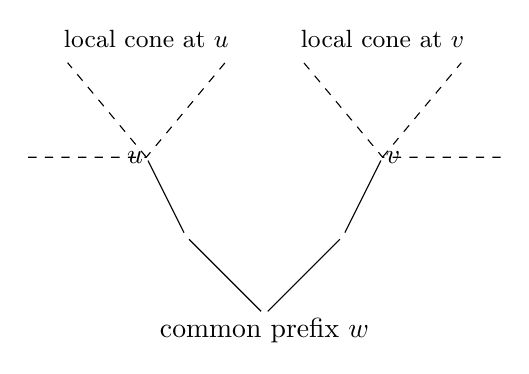
\begin{tikzpicture}[scale=1.0, every node/.style={inner sep=1pt}]
  % Common causal past
  \node (root) at (0,0) {};
  \node (a1) at (-1,1) {};
  \node (b1) at (1,1) {};

  % Two divergent prefixes u and v
  \node (u) at (-1.5,2) {};
  \node (v) at (1.5,2) {};

  % Subcones below u
  \draw[dashed] (-3,2) -- (-1.5,2) -- (-0.5,3.2);
  \draw[dashed] (-1.5,2) -- (-2.5,3.2);

  % Subcones below v
  \draw[dashed] (3,2) -- (1.5,2) -- (0.5,3.2);
  \draw[dashed] (1.5,2) -- (2.5,3.2);

  % Edges in prefix tree
  \draw (root) -- (a1);
  \draw (root) -- (b1);
  \draw (a1) -- (u);
  \draw (b1) -- (v);

  % Labels
  \node[left] at (-1.5,2) {$u$};
  \node[right] at (1.5,2) {$v$};
  \node[below] at (0,0) {common prefix $w$};

  \node at (-1.5,3.5) {\small local cone at $u$};
  \node at (1.5,3.5) {\small local cone at $v$};
\end{tikzpicture}

			\caption{Two Dyck prefixes $u$ and $v$ diverging from a shared ancestor $w$.
				Dashed regions indicate the local Catalan cones rooted at $u$ and $v$.
				Cones nest along causal chains and diverge after branching points, producing
			a family of local, relocatable causal geometries on the Catalan substrate.}
	\label{fig:multiple-cones}
\end{figure}

\subsection{Summary}
The Catalan substrate supports a discrete causal geometry determined entirely
by recursive constraint. Without introducing a manifold, metric, or causal
relation by fiat, it yields:
\begin{itemize}
	\item a partial order interpretable as causality,
	\item a cone-shaped causal envelope,
	\item intrinsic bounds on spatial extension,
	\item well-defined constant-time layers.
\end{itemize}
Subsequent sections place dynamical rules---computational reduction and a
minimal amplitude calculus---on this geometry.

\section{Recursive Pairing and Universal Computation}
\label{sec:computation}

\noindent
We now read the same Catalan objects from the computational side. The
correspondence between binary application trees and applicative calculi is
classical \cite{church33,CurryFeys1958,barendregt84}; our purpose is to emphasize
that computation, like causal growth and amplitude dynamics, can be expressed
through pair-local operations on the same substrate. This will later motivate
the gauge-equivalence viewpoint of Section~\ref{sec:locality}. Full binary trees
serve as application frames, while pairs encodings provide a uniform
parentheses-only syntax. The only additional choice needed to represent concrete
programs is an encoding of symbols at leaves.

\subsection{Pairs expansion}

\paragraph{Catalan shapes as program frames.}

The Catalan family (Dyck paths, full binary trees, and balanced parentheses)
forms the free magma on a single binary constructor: it is the
space of all finite binary application frames. As observed in classical
treatments of the $\lambda$-calculus and combinatory logic
\cite{CurryFeys1958,barendregt84}, application is binary, so every SKI term (and
every $\lambda$-term after fixing a binding convention) has a canonical
representation as a finite binary application tree: internal nodes encode
application; leaves encode atomic symbols (variables, constants, or combinators).
Conversely, any finite binary tree equipped with leaf labels denotes a unique
applicative term over that alphabet, modulo surface syntax. Since SKI is
computationally universal, this yields an explicit embedding of all computable
programs (as terms) within the Catalan substrate. The apparent choice of leaf
alphabet can itself be internalized by representing symbols as distinguished
Catalan motifs (Remark~\ref{rem:symbol-motifs}).

	\begin{remark}[Symbols as Distinguished Motifs]
	\label{rem:symbol-motifs}
		Although we sometimes describe leaf labels as an external choice, one may work
		in a purely structural setting: there is an injective encoding of labeled
		application trees (and in particular SKI terms) into unlabeled Catalan trees by
		tagging constructor nodes and representing each symbol by a fixed subtree motif.
		An explicit construction is recorded in Appendix~\ref{appendix:computational-foundations}.
		\end{remark}

This observation also extends to operational semantics. Standard reductions
(such as $\beta$-reduction or SKI contraction) are local rewrite rules on binary
trees, and the pairs-expansions of combinators remain within the Catalan family.
Accordingly, a program, its intermediate expansion frames, and each permissible
reduction schedule are all representable as paths through a single Catalan
substrate. Selecting a program shape or selecting a specific reduction history
is therefore equivalent to selecting a path in the Catalan tree. In this sense
the Catalan substrate uniformly encodes program syntax, program semantics, and
the full ensemble of admissible computational histories.

	\begin{proposition}[Catalan Universality for Program Structure]
		\label{prop:catalan-programs}
		Let $\mathcal{T}$ denote the Catalan family of finite full binary trees.
		Every program in any Turing-complete functional calculus (such as the
		$\lambda$-calculus or SKI) admits a canonical representation as an element of
		$\mathcal{T}$ with leaf labels drawn from a finite alphabet (after fixing a
		standard encoding of symbols). Conversely,
		every labeled element of $\mathcal{T}$ denotes a unique program modulo surface
		syntax. Furthermore, standard operational semantics (including
		$\beta$-reduction and SKI contraction) act as local rewrite rules that
		preserve membership in $\mathcal{T}$. Thus a program, its syntactic
	expansions, and every admissible reduction history correspond to paths within
	the Catalan substrate.
	\end{proposition}
	\noindent
	\begin{proof}[Proof sketch]
	As described in classical treatments of combinatory logic and the
	$\lambda$-calculus \cite{CurryFeys1958,barendregt84}, application is a binary
	operation, so every term admits a unique representation as a full binary tree:
	internal nodes encode application and leaves encode atomic symbols (after
	fixing a standard encoding of symbols/variables). Conversely, any labeled full
	binary tree denotes a unique applicative term modulo surface syntax.
	Operational semantics (e.g.\ $\beta$-reduction and SKI contraction) act as
	local pattern-rewrite rules on such trees and preserve the class of full binary
	trees. Thus a program, its syntactic expansions, and each admissible reduction
	history correspond to paths in the induced multiway rewrite graph on
	$\mathcal{T}$.
	\end{proof}

\paragraph{Two parentheses encodings.}
Two particularly useful parentheses-only encodings of a full binary tree are:

\begin{itemize}
  \item \textbf{Dyck encoding} (``walk'' view): balanced parentheses of length
    $2n$, naturally adapted to height profiles and scaling limits.
  \item \textbf{Pairs (S-expression) encoding} (``cons'' view): write each leaf
    as \texttt{()} and each internal node as a parenthesized pair of its two
    children, i.e.\ $T=(L,R)\mapsto (\texttt{enc}(L)\,\texttt{enc}(R))$.  This is
    a variable- and label-free Lisp-style representation with \texttt{()} as the
    only atom.
\end{itemize}

	In particular, in the \emph{pairs} encoding, the smallest object is the empty
	pair \texttt{()}, and the smallest nontrivial \emph{binary} object is
	\texttt{(()())}, i.e.\ a root pair whose two children are leaves.  In the Dyck
	encoding, the semilength-$1$ object is \texttt{()}, since Dyck words begin only
	after the first matched pair exists.

\paragraph{Handedness and path selection.}
The Dyck constraint (including return to height $0$ at completion) is a
well-bracketing discipline: it constrains which histories are admissible, but
it does not by itself impose a within-tier ordering of alternatives or select a
dynamic among them. By contrast, the applicative reading of Catalan trees as
programs requires that internal nodes represent \emph{ordered} pairs
(function, argument), i.e.\ one must fix a convention (e.g.\ ``left applies to
right''). This handedness determines syntax, but not which computational history
is realized among many permissible ones: selecting a computation corresponds to
choosing a reduction strategy (or, in a stochastic formulation, a transition
kernel) on the same Catalan substrate.

\subsection{A small tier shown three ways (Dyck / tree / pairs)}
Figure~\ref{fig:trees-n3-tikz} augments the standard Dyck-$n=3$ list by
displaying, for the \emph{same} five Catalan shapes, the corresponding pairs
(S-expression) encodings. For concreteness, the five shapes are listed
left-to-right in lexicographic order on Dyck words (with \texttt{(} $<$ \texttt{)}),
and the tree and pairs rows are obtained by the standard bijection.

	\begin{figure}[H]
	  \centering
	  \input{figures/clc-trees-n3-tikz.tex}
	  \caption{The five Catalan shapes at tier $n=3$ shown as (i) full binary trees,
	  together with (ii) Dyck words and (iii) pairs (S-expression) encodings in which each
	  leaf is \texttt{()} and each internal node is a parenthesized pair of its two
	  children (as if one were looking "down into" the tree). These are three
  coordinate systems for the same underlying Catalan objects.}
  \label{fig:trees-n3-tikz}
\end{figure}

\subsection{Connection to \texorpdfstring{$\lambda$}{lambda}-calculus and SKI}

Full binary trees are a standard representation of SKI terms, and they capture
the application skeleton of $\lambda$-terms \cite{church33,CurryFeys1958,barendregt84}.
A full $\lambda$-encoding requires a binding convention (e.g.\ variables as leaf
labels or positions, and abstraction as a structural marker), while application
is encoded by the tree's binary node. Under the pairs expansion, each Dyck tree canonically determines an
unlabeled application graph. When variables are suppressed, the resulting graphs
coincide with the structure graphs used in combinatory logic. No additional
primitives beyond recursive pairing are required to obtain this representation.

Choosing a finite set of tree patterns to represent the SKI combinators and
interpreting local tree rewrites as SKI reduction therefore equips the Catalan
substrate with a standard universal calculus: every partial recursive function
can be encoded as an SKI term \cite{CurryFeys1958,barendregt84}, and hence by a
finite Dyck tree, and every computation corresponds to a sequence of local tree
	transformations. In this
	sense, the Catalan substrate is \emph{computationally universal}. We use this
	standard universality fact to emphasize that computation can be expressed by
	pair-local rewrites on the same Catalan objects that carry the causal prefix
	order.

\subsection{Reduction and local collapse}

In the computational interpretation, reduction corresponds to local pattern
replacement. A redex occupies a finite region of a tree and may be reduced
without reference to distant subtrees. This locality mirrors the causal
structure established in Section~\ref{sec:catalan_cone}. From the perspective
of the Catalan lattice, reduction may be viewed as \emph{collapse}: a locally
ambiguous structure is replaced by a simpler one consistent with the global
constraint. Importantly, collapse does not alter causal ancestry; it refines an
already-admissible history. For standard calculi (e.g.\ $\lambda$/SKI),
confluence ensures uniqueness of normal forms when they exist, and more locally
reductions supported on disjoint subtrees commute \cite{barendregt84}. This computational fact will
later support an interpretation of spacelike commutativity.

\subsection{Summary}

Recursive pairing suffices to encode universal computation. Via the pairs
expansion, Dyck trees and application graphs are two views of the same
structure. Local computational reduction aligns naturally with causal locality
on the Catalan light cone.

\section{Quantum Amplitudes on the Catalan Lattice}
\label{sec:amplitudes}

\noindent
This section defines a minimal amplitude calculus on the Catalan history space.
The key inputs are (i) a coarse-graining/observable $f$ identifying which
histories are regarded as the same outcome, and (ii) a choice of additive phase
functional on histories. Given these, we assign complex phase weights, define
amplitudes by coherent summation over preimages, and read out probabilities by
normalized squared magnitudes, in analogy with the Born rule \cite{feynman-hibbs65}.
The phase functional is constrained here only by the pairs-only locality discipline
(Proposition~\ref{prop:phase-classification}).

	\paragraph{Configuration space versus readout.}
	At fixed tier $n$, the set $\mathcal D_n$ is a \emph{configuration space} of
	completed histories. A ``screen coordinate'' (or any measurement outcome) is not
	identified with $\mathcal D_n$ itself, but with an \emph{observable} (deterministic
	coarse-graining) $f:\mathcal D_n\to\mathcal X$ to an outcome set $\mathcal X$,
	chosen to model a measurement protocol. Likewise, intrinsic chart variables
	attached to histories (e.g.\ height along a prefix trajectory, or history-level
	statistics such as breadth $b(w)$) become readouts only when selected as part of $f$.
	When a concrete detector coordinate is needed, our default choice is a
	height-at-slice readout (Appendix~\ref{appendix:doubleslit}).

\begin{definition}[Catalan amplitude model at fixed tier]
\label{def:catalan-amplitude-model}
Fix a tier $n$ and an observable (coarse-graining) $f:\mathcal D_n\to\mathcal X$
to a finite outcome set $\mathcal X$. Fix a real phase functional
$\Phi:\mathcal D_n\to\mathbb R$, a scale $\alpha\in\mathbb R$, and (optionally)
a magnitude function $\rho:\mathcal D_n\to\mathbb R_{\ge 0}$. Define per-history
amplitudes
\[
\psi(w):=\rho(w)\,e^{i\alpha \Phi(w)}\in\mathbb C,
\]
where the minimal unit-modulus case is $\rho\equiv 1$.
The outcome amplitude and normalized probability are
\[
\Psi(x):=\sum_{w:\,f(w)=x}\psi(w),
\qquad
P(x):=\frac{|\Psi(x)|^2}{\sum_{x'\in\mathcal X}|\Psi(x')|^2},
\]
whenever the denominator is nonzero.
\end{definition}

In what follows we specialize Definition~\ref{def:catalan-amplitude-model} to
unit magnitude $\rho\equiv 1$ and emphasize additive phase functionals, with the
Dyck area $A(w)$ as the main example.

\subsection{Histories as paths}

Interpreting Dyck paths as admissible histories motivates assigning weights to
each history.  Let $\mathcal{D}_n$ denote the set of Dyck paths of tier $n$. A
state at tier $n$ may be represented as a formal superposition of histories

\[
	\Psi_n = \sum_{w \in \mathcal{D}_n} \psi(w)\,|w\rangle .
\]

Local extensions of a Dyck path correspond to admissible future steps. Thus,
time evolution is governed by transitions that respect the Dyck constraint.

\subsection{Observables, projection, and coherent summation}

Fix a tier $n$ and consider the set $\mathcal D_n$ of Dyck paths of semilength
$n$. Each $w\in\mathcal D_n$ represents a complete admissible history at discrete
time $n$, with an associated height profile
\[
	H_w : \{0,1,\dots,2n\} \to \mathbb Z_{\ge 0}.
\]
An observable is defined as a deterministic coarse-graining
\[
	f : \mathcal D_n \to \mathcal X,
\]
where $\mathcal X$ is a discrete set of outcomes corresponding to a chosen
equivalence relation on histories. An outcome $x\in\mathcal X$ corresponds to
the equivalence class $f^{-1}(x)\subset\mathcal D_n$ of histories.  By
construction, such a projection discards information: many distinct histories
may be identified as the same observable outcome.

With no additional structure imposed, the natural measure on $\mathcal D_n$ is
uniform counting. The induced distribution on the outcome space $\mathcal X$ is
therefore the pushforward of the uniform counting measure,
\[
	N(x) := \#\{w\in\mathcal D_n : f(w)=x\}.
\]
\begin{remark}[Local observables and counting recursions]
\label{rem:local-observables}
For pairs-only models, one typically restricts attention to coarse-grainings $f$
that are computable online from bounded prefix-local data along Dyck growth (for
example, by a finite-state transducer driven by the current height and step
type). For such $f$, the multiplicities $N(x)$ may be computed by transfer-matrix
recursions on the induced state space. We keep $f$ arbitrary here for
generality.
\par
Independently of any chosen observable, the Dyck growth process admits a canonical
state compression: the rooted future cone of a prefix depends only on its current
height (Lemma~\ref{lem:cone-iso-height}), and for a fixed completion horizon the
number of admissible completions depends only on remaining steps and height
(Lemma~\ref{lem:ballot-completions}). This yields the time-inhomogeneous
Dyck-conditioned Markov kernel of Lemma~\ref{lem:dyck-conditioned-kernel}, in
which the next step is chosen with probability proportional to the number of
admissible futures after taking that step.
\end{remark}
\begin{remark}[Coherent vs.\ counting aggregation]
In the uniform counting baseline, the probability of an outcome is proportional
to $N(x)$. In the Catalan amplitude model (Definition~\ref{def:catalan-amplitude-model})
with unit magnitude $\rho\equiv 1$, if the phase functional factors through the
observable (i.e.\ $\Phi=\widetilde{\Phi}\circ f$, so all histories in $f^{-1}(x)$
have the same phase), then
\[
\Psi(x)=e^{i\alpha\widetilde{\Phi}(x)}\,N(x)
\qquad\Rightarrow\qquad
P(x)\propto N(x)^2.
\]
Destructive/constructive interference occurs only when $\Phi$ varies within the
fibers $f^{-1}(x)$.

At the opposite extreme, if one models the phases within each fiber as
independent uniform random variables (a purely mathematical phase-scrambling
toy model), then the unnormalized weights revert to multiplicity in expectation:
writing $\Psi(x)=\sum_{j=1}^{N(x)} e^{i\Theta_j}$ with $\Theta_j\stackrel{\mathrm{iid}}{\sim}\mathrm{Unif}[0,2\pi)$,
one has
\[
\mathbb E\bigl[|\Psi(x)|^2\bigr]=N(x),
\]
since the cross terms average to $0$ by independence and rotational symmetry.
\end{remark}
Even with uniform weight on histories, the induced distribution on $\mathcal X$
is generically non-uniform, reflecting the combinatorial geometry of the
projection rather than any imposed dynamics.

A discrete analogue of an integral along a history is given by the step-sum of
the height profile,
				\[
					A(w) := \sum_{k=0}^{2n-1} H_w(k),
			\]
			which measures the cumulative dwell time at nonzero height. This quantity
			depends on the full distribution of height along the path, not merely on
			extrema such as maximum height or peak count.

\begin{remark}[Area as a step-additive functional]
The functional $A(w)$ is computed online by maintaining the current height and
accumulating it, and is therefore of the step-additive form of
Proposition~\ref{prop:phase-classification}.
\end{remark}

\begin{lemma}[Area as sum of pair lifetimes]
\label{lem:area-pair-lifetimes}
Let $w=w_1\cdots w_{2n}\in\mathcal D_n$ and let $A(w)=\sum_{k=0}^{2n-1}H_w(k)$ as
above. For each matched pair $p$ of parentheses in $w$, let $i(p)<j(p)$ be the
positions of its opening and closing symbols. Then
\[
A(w)=\sum_{p}\bigl(j(p)-i(p)\bigr).
\]
In particular, $A(w)$ decomposes as a sum of contributions associated to
individual pairs.
\end{lemma}

\begin{proof}
For each $k\in\{0,\dots,2n-1\}$, the height $H_w(k)$ equals the number of pairs
whose opening has occurred but whose closing has not yet occurred. A fixed pair
$p$ contributes $1$ to $H_w(k)$ exactly for $k=i(p),\dots,j(p)-1$, a set of size
$j(p)-i(p)$. Double counting yields the identity.
\end{proof}

				\begin{remark}[Area refinement and $q$-Catalan weights]
				Under the standard identification of Dyck paths with lattice paths from
				$(0,0)$ to $(n,n)$ staying above the diagonal, the usual \emph{area} statistic
			$\mathrm{area}(w)$ (counting unit squares between the path and the diagonal)
		satisfies $\mathrm{area}(w)=(A(w)-n)/2$, i.e.\ $A(w)=n+2\,\mathrm{area}(w)$.
		Consequently, the weighted sum of the area phase is a specialization of the
		area-refined Catalan generating function:
		\[
		\sum_{w\in\mathcal D_n} e^{i\alpha A(w)}
		=
		e^{i\alpha n}\sum_{w\in\mathcal D_n}\bigl(e^{2i\alpha}\bigr)^{\mathrm{area}(w)}.
		\]
		In particular, any analytic information about the distribution of Dyck area
		and its generating functions may be transferred directly to these phase-weighted
			sums \cite{stanley-catalan,janson07}.
			\end{remark}

		\begin{definition}[Area-weighted nonnegative bridge kernel]
		\label{def:area-weighted-bridge}
		Fix $\alpha\in\mathbb R$. For $r\ge 0$ and $a,b\in\mathbb Z_{\ge 0}$, define
		$K_\alpha^{(r)}(a,b)$ to be the complex weight-sum over all length-$r$
		$\pm 1$ paths $(h_0,\dots,h_r)$ such that $h_0=a$, $h_r=b$, $h_t\ge 0$ for all
		$t$, and $h_{t+1}-h_t\in\{\pm 1\}$, with weight
		\[
		\exp\!\Big(i\alpha\sum_{t=0}^{r-1} h_t\Big).
		\]
		\end{definition}

		\begin{lemma}[Transfer recursion and composition for the area phase]
		\label{lem:area-transfer}
		The kernels $K_\alpha^{(r)}$ satisfy:
		\begin{enumerate}[label=(\roman*)]
		\item \textbf{Initial condition:} $K_\alpha^{(0)}(a,b)=\mathbf 1_{\{a=b\}}$.
		\item \textbf{One-step recursion:} for $r\ge 0$ and $a,b\ge 0$,
		\[
		K_\alpha^{(r+1)}(a,b)
		=
		e^{i\alpha a}\Big(K_\alpha^{(r)}(a+1,b)+K_\alpha^{(r)}(a-1,b)\Big),
		\]
		with the convention $K_\alpha^{(r)}(-1,b)=0$.
		\item \textbf{Chapman--Kolmogorov (semigroup) property:} for $r,s\ge 0$ and
		$a,c\ge 0$,
		\[
		K_\alpha^{(r+s)}(a,c)=\sum_{b\ge 0} K_\alpha^{(r)}(a,b)\,K_\alpha^{(s)}(b,c).
		\]
		\end{enumerate}
		In particular, the area-phase partition function at tier $n$ is
		\[
		Z_n(\alpha):=\sum_{w\in\mathcal D_n} e^{i\alpha A(w)} = K_\alpha^{(2n)}(0,0),
		\]
		so $Z_n(0)=C_n$.
		\end{lemma}

			\begin{proof}[Proof sketch]
				For (ii), condition on the first step from height $a$ to $a\pm 1$: the first
				step contributes the factor $e^{i\alpha a}$, and the remaining $r$ steps are
				counted by $K_\alpha^{(r)}(a\pm 1,b)$. The boundary convention encodes the
				nonnegativity constraint via $K_\alpha^{(r)}(-1,b)=0$.

			For (iii), split a length-$(r+s)$ path at time $r$. The area functional
			$\sum_{t=0}^{r+s-1} h_t$ is additive under this concatenation, so the weight
			factors as the product of the two segment weights. Summing over the
			intermediate height $b=h_r$ yields the stated composition law.
			\end{proof}

			\begin{remark}[Transfer-operator form]
			\label{rem:area-transfer-operator}
			Define an infinite matrix $\mathcal{M}_\alpha$ on $\mathbb Z_{\ge 0}$ by
			\[
			(\mathcal{M}_\alpha)_{a,c}
			:=e^{i\alpha a}\Big(\mathbf 1_{\{c=a+1\}}+\mathbf 1_{\{c=a-1\}}\Big),
			\]
			with the convention $\mathbf 1_{\{c=-1\}}=0$. Then the kernel in
			Definition~\ref{def:area-weighted-bridge} is the $r$th matrix power:
			\[
			K_\alpha^{(r)}(a,b) = (\mathcal{M}_\alpha^r)_{a,b}.
			\]
			In particular, Lemma~\ref{lem:area-transfer} is the statement that
			$\mathcal{M}_\alpha^{r+s}=\mathcal{M}_\alpha^{r}\mathcal{M}_\alpha^{s}$ and
			$K_\alpha^{(r+1)}=\mathcal{M}_\alpha K_\alpha^{(r)}$.
			\end{remark}

			\begin{lemma}[First-return recursion for the area phase]
			\label{lem:area-first-return}
			Let $Z_n(\alpha):=\sum_{w\in\mathcal D_n} e^{i\alpha A(w)}$ as in
			Lemma~\ref{lem:area-transfer}. Then $Z_0(\alpha)=1$, and for $n\ge 1$,
		\[
		Z_n(\alpha)
		=
		\sum_{k=0}^{n-1} e^{i\alpha(2k+1)}\,Z_k(\alpha)\,Z_{n-1-k}(\alpha).
		\]
		Equivalently, writing $q:=e^{2i\alpha}$ and
		$C_n(q):=\sum_{w\in\mathcal D_n} q^{\mathrm{area}(w)}$, one has $C_0(q)=1$ and
		for $n\ge 1$,
		\[
		C_n(q)=\sum_{k=0}^{n-1} q^{k}\,C_k(q)\,C_{n-1-k}(q),
		\]
		the Carlitz--Riordan recursion for the area-refined Catalan numbers.
		\end{lemma}

		\begin{proof}[Proof sketch]
		Every nonempty Dyck word $w\in\mathcal D_n$ admits a unique first-return
		decomposition
		\[
		w=\texttt{(}\,u\,\texttt{)}\,v,
		\]
		where $u\in\mathcal D_k$ and $v\in\mathcal D_{n-1-k}$ for a unique
		$k\in\{0,\dots,n-1\}$. A direct height bookkeeping shows
		$A(w)=A(u)+A(v)+(2k+1)$, so $e^{i\alpha A(w)}=e^{i\alpha(2k+1)}e^{i\alpha A(u)}e^{i\alpha A(v)}$.
		Summing over $u$ and $v$ at fixed $k$ yields the stated recursion for $Z_n$.
		The $q$-form follows from $\mathrm{area}(w)=(A(w)-n)/2$ and the same
		decomposition; see \cite{stanley-catalan}.
		\end{proof}

		\begin{corollary}[Functional equation for the area-refined generating function]
		\label{cor:q-catalan-functional-equation}
		Let $C(q;z):=\sum_{n\ge 0} C_n(q)\,z^n$, where $C_n(q)$ is as in
		Lemma~\ref{lem:area-first-return}. Then
		\[
		C(q;z)=1+z\,C(q;z)\,C(q;qz).
		\]
		\end{corollary}

		\begin{proof}
		Multiply the recurrence for $C_n(q)$ in Lemma~\ref{lem:area-first-return} by
		$z^n$ and sum over $n\ge 1$. Writing $n-1=k+m$ gives
		\[
		C(q;z)-1
		= \sum_{k,m\ge 0} q^k\,C_k(q)\,C_m(q)\,z^{k+m+1}
			= z\,C(q;qz)\,C(q;z).
			\]
			\end{proof}

			\begin{corollary}[Stieltjes continued fraction]
			\label{cor:q-catalan-continued-fraction}
			As a formal power series in $z$, the solution $C(q;z)$ of
			Corollary~\ref{cor:q-catalan-functional-equation} admits the continued-fraction
			expansion
			\[
			C(q;z)
			=
			\cfrac{1}{1-\cfrac{z}{1-\cfrac{qz}{1-\cfrac{q^{2}z}{1-\ddots}}}}.
			\]
			\end{corollary}

			\begin{proof}[Proof sketch]
			Rearranging Corollary~\ref{cor:q-catalan-functional-equation} gives
			$C(q;z)=1/(1-z\,C(q;qz))$. Applying the same identity with $z$ replaced by
			$qz$ yields $C(q;qz)=1/(1-qz\,C(q;q^2z))$, and iterating produces the stated
			continued fraction.
			\end{proof}

			\begin{remark}
			Equivalently, define $Z(\alpha;z):=\sum_{n\ge 0} Z_n(\alpha)\,z^n$. Since
			$Z_n(\alpha)=e^{i\alpha n}C_n(e^{2i\alpha})$, one has
			\[
		Z(\alpha;z)=C(e^{2i\alpha};e^{i\alpha}z),
		\]
		and therefore $Z(\alpha;z)$ satisfies
		\[
		Z(\alpha;z)=1+e^{i\alpha}z\,Z(\alpha;z)\,Z(\alpha;e^{2i\alpha}z).
		\]
		\end{remark}

		\begin{remark}[Discrete Feynman--Kac viewpoint]
		The recursion in Lemma~\ref{lem:area-transfer} is a transfer-matrix
		formulation for a nearest-neighbour walk with a multiplicative potential
		term $e^{i\alpha h}$. Under diffusive scaling, this is the discrete analogue
		of inserting an exponential of a time-integrated potential, as discussed in
		Section~\ref{subsec:phase-scaling} \cite{kac49}.
		\end{remark}

		More generally, one may use any \emph{additive} functional on Dyck histories as
		a phase source, provided it is computable online from prefix-local growth
		information. The following proposition records the general form of such
		functionals.

	\begin{proposition}[Additive phase functionals computable along Dyck growth]
	\label{prop:phase-classification}
	Let $w$ be a Dyck history of semilength $n$, and let $(X_t)_{t=0}^{2n-1}$
	denote the sequence of \emph{prefix-local} growth states along $w$ (e.g.\
	current height and step type). For Dyck histories $u,v$ define concatenation
	$uv$ as the concatenation of Dyck words.

	A real-valued functional $\Phi(w)$ is additive under Dyck concatenation, i.e.\
	$\Phi(uv)=\Phi(u)+\Phi(v)$, and computable online by a (possibly
	countable-state) Markov transducer driven by $(X_t)$ with fixed initial
	internal state $Y_0=y_\ast$ for every history, if and only if there exist an
	internal state process $(Y_t)$ with update rule $Y_{t+1}=F(Y_t,X_t)$ and a
	real-valued increment function $g$ such that
	\[
		\Phi(w) \;=\; \sum_{t=0}^{2n-1} g(Y_t,X_t).
	\]

	Equivalently, defining the augmented prefix-local state $Z_t := (X_t,Y_t)$,
	one has
	\[
		\Phi(w) \;=\; \sum_{t=0}^{2n-1} \varphi(Z_t)
	\]
	for some function $\varphi$ on the augmented state space.
	\end{proposition}

	\begin{proof}[Proof sketch]
	Immediate: an online additive transducer emits a per-step output $g(Y_t,X_t)$,
	whose sum over the growth process defines $\Phi$; conversely, any such per-step
	sum is computable by an online transducer with internal state $(Y_t)$.
	\end{proof}

	\begin{remark}
	In the special case where the transducer carries no internal state (i.e.\
	$Y_t$ is trivial) and the prefix-local state is taken to be the current height
	$h_t$, the admissible phase functionals are precisely those of the form
	\[
		\Phi_f(w) = \sum_{t} f(h_t),
	\]
	for some function $f : \mathbb Z_{\ge 0} \to \mathbb R$. Allowing dependence on
	step type yields the slightly more general form $f(h_t,\Delta h_t)$. The area
	functional corresponds to the choice $f(h)=h$.
	\end{remark}

	Specializing to the area functional $A(w)$, one may define a complex phase
	\[
	\theta(w) := \alpha\,A(w),
	\qquad
	\psi(w) := e^{i\theta(w)},
\]
where $\alpha$ is a global scale parameter. No per-path phase assignment is
introduced; distinct phases arise solely from differences in the distribution of
height over the history.

Given an observable $f$, the complex amplitude associated with an outcome
$x\in\mathcal X$ is the coherent sum
\[
\Psi(x) := \sum_{w:\,f(w)=x} \psi(w),
\]
and observed probabilities are obtained by normalization of squared magnitudes,
\[
P(x) = \frac{|\Psi(x)|^2}{\sum_{x'\in\mathcal X}|\Psi(x')|^2}.
\]
Thus histories that are indistinguishable under the observable $f$ are combined
prior to squaring, while distinguishable histories are not. Interference is
therefore a generic consequence of assigning complex weights to histories and
summing coherently over coarse-grained equivalence classes before applying the
Born rule.

\paragraph{Optional: coarse-graining entropy.}
Appendix~\ref{appendix:technical-notes} records optional entropy bookkeeping for
coarse-grainings and collapse counts.

\subsection{Path integrals and conditioned walks}

Dyck paths are random walks conditioned to remain nonnegative and return to
zero. Classical results show that, when rescaled appropriately, ensembles of
such paths converge to Brownian excursions \cite{le-gall05,janson07}.
Assigning equal weight to all admissible paths yields a discrete analogue of a
path integral \cite{feynman-hibbs65}.
More general amplitude assignments may depend on other prefix-local features
(e.g.\ height, step type, or other additive functionals), provided the Dyck
constraint is preserved.

	\begin{figure}[ht]
		\centering
		\begin{tikzpicture}[scale=0.7]
  % axes
  \draw[->] (0,0) -- (13,0) node[below] {$k$};
  \draw[->] (0,0) -- (0,6) node[left] {$H_k$};

  % sample Dyck path (semilength 6)
  \draw[thick]
    (0,0) -- (1,1) -- (2,2) -- (3,3) -- (4,2) -- (5,3) -- (6,4)
    -- (7,3) -- (8,2) -- (9,3) -- (10,2) -- (11,1) -- (12,0);

  % labels
  \node[below] at (0,0) {0};
  \node[below] at (12,0) {$2n$};
  \node[above right] at (3,3) {\small Dyck walk};

  % schematic smooth excursion overlay
  \draw[dashed] plot[smooth] coordinates {
    (0,0) (2,1) (4,2.8) (6,4.2) (8,2.5) (10,1.2) (12,0)
  };
  \node[right] at (12,4.2) {\small Brownian excursion (scaling limit)};
\end{tikzpicture}

		\caption{A Dyck path as a nearest-neighbour walk $(H_k)$ constrained to stay
			nonnegative and return to zero at time $2n$.
			Under diffusive rescaling of $k$ and $H_k$, ensembles of such paths converge
			to Brownian excursions, providing the bridge to the heat and Schr\"odinger
	equations discussed in the text.}
	\label{fig:dyck-walk-excursion}
\end{figure}

\subsection{Discrete path-integral formulation}

The preceding constructions admit a direct interpretation as a discrete path
integral on the Catalan light cone. Fix a tier $n$ and an observable
$f:\mathcal D_n\to\mathcal X$, where $\mathcal X$ is a finite set of outcomes
corresponding to a chosen coarse-graining of histories. Each Dyck path
$w\in\mathcal D_n$ represents a complete admissible history, and the projection
$f$ determines which distinctions between histories are retained and which are
discarded.

Define a complex weight for each history by
\[
\psi(w) = e^{i\alpha A(w)},
\]
where
\[
A(w) = \sum_{k=0}^{2n-1} H_w(k)
\]
is the discrete height integral introduced above. The amplitude associated with
an observable outcome $x\in\mathcal X$ is then
\[
\Psi(x) = \sum_{w:\,f(w)=x} e^{i\alpha A(w)}.
\]


This expression is formally analogous to a path integral \cite{feynman-hibbs65}:
the amplitude is a sum over all admissible histories compatible with the
observable outcome, with each history contributing a phase determined by an
additive functional. No continuum limit, action functional, or variational
principle is assumed at this stage; the structure arises purely from discrete
combinatorics.

Several features commonly associated with continuum path integrals are already
present:

\begin{enumerate}[label=(\roman*)]
\item \textbf{Sum over histories.}
All admissible Dyck paths consistent with the observable contribute. The Dyck
constraint enforces causal admissibility in the same way that restrictions on
allowed paths do in relativistic path integrals.

\item \textbf{Additive phase functional.}

The quantity $A(w)$ is additive under concatenation of path segments and depends
only on the local height increments. It therefore plays the role of a discrete
action accumulated along the history.

\item \textbf{Interference from coarse-graining.}
Interference arises precisely because the observable $f$ fails to distinguish
between certain histories. Histories that are identified by the projection are
summed coherently, while those distinguished by the observable are not.

\end{enumerate}

From this perspective, the Catalan lattice provides a discrete realization of
the sum-over-histories principle in which both the space of histories and the
phase functional are combinatorially well defined. In the next subsection we
show that, under appropriate scaling limits, this discrete formulation admits a
diffusion (heat) continuum limit (Section~\ref{sec:continuum-limit}); the same
Laplacian generator also yields the free Schr\"odinger equation under analytic
continuation (Section~\ref{subsec:schrodinger}).

Measurement-like coarse observations may be modeled by choosing observables that
retain geometric features of a history (such as transverse displacement at a
fixed tier). No such spatial interpretation, however, is required for the
formal development.

For readers seeking a concrete intuition for how this discrete
sum-over-histories mechanism produces interference,
Appendix~\ref{appendix:doubleslit} sketches a finite thought experiment
analogous to the double-slit experiment. The worked example also makes
explicit that coherent phase-weighted summation can shift $|\Psi(x)|^2$
substantially away from the raw multiplicities $N(x)$, even at finite tier.

\subsection{Scaling of the area phase in the continuum limit}
\label{subsec:phase-scaling}

The interference mechanism above assigns each history $w\in\mathcal D_n$ a
complex weight $\psi(w)=e^{i\alpha A(w)}$ with discrete area functional
\[
A(w) := \sum_{k=0}^{2n-1} H_w(k),
\]
where $H_w(k)$ is the height after $k$ steps.

To relate this discrete phase to the diffusion scaling limit, introduce the
rescaled height process on $[0,1]$,
\[
X^{(n)}(\tau) := n^{-1/2} H_w(\lfloor 2n\tau\rfloor), \qquad 0\le \tau \le 1.
\]
	Under the standard Donsker-type invariance principle for Dyck paths (conditioned
	random walks), $X^{(n)} \Rightarrow X$ in distribution, where $X$ is a Brownian
	excursion on $[0,1]$ \cite{le-gall05,janson07}.

	The discrete area rescales as a Riemann sum:
	\[
	\frac{1}{2n^{3/2}}A(w)
	= \frac{1}{2n}\sum_{k=0}^{2n-1} n^{-1/2}H_w(k)
	\;\Longrightarrow\;
	\int_0^1 X(\tau)\,d\tau.
	\]
	The factor $2$ reflects that a Dyck history of semilength $n$ has $2n$ steps,
	so $1/(2n)$ is the natural Riemann-sum normalization over $\tau\in[0,1]$.
Consequently, a nontrivial continuum phase is obtained by scaling $\alpha$ with
$n$ as
\[
\alpha_n := \frac{\lambda}{2n^{3/2}},
\]
so that
\[
e^{i\alpha_n A(w)}
\;\Longrightarrow\;
\exp\!\Big(i\lambda\int_0^1 X(\tau)\,d\tau\Big).
\]

This makes explicit that the discrete coherent sum with additive functional
$A(w)$ converges to a continuum functional weight. In particular, when one
passes from uniform counting of conditioned walks to diffusion limits, inserting
the exponential of a time-integrated functional corresponds (at the PDE level)
to adding a potential term (via the standard Feynman--Kac mechanism
\cite{kac49}). Setting $\lambda=0$ recovers the unweighted scaling limit
discussed in the next subsection.

\subsection{Diffusion limit}
\label{sec:continuum-limit}

Let $n\to\infty$ and rescale time and height by

\[
	t \mapsto n\tau, \qquad h \mapsto \sqrt{n}\,x .
\]

	Under the standard Donsker-type invariance principle for conditioned simple
	random walks (equivalently, uniform Dyck paths), the rescaled height process
	converges in law to a Brownian excursion on $x\ge0$. At the PDE level, the
	diffusion part is governed
	by the heat operator on the half-line, while the Dyck constraint is imposed by
	conditioning (a Doob transform / Bessel-bridge representation) rather than by a
	time-homogeneous boundary condition alone. In particular, the corresponding
	diffusion term on $x>0$ is the half-line Laplacian,

\[
L := \frac{1}{2}\,\partial_x^2.
\]

\begin{remark}[Discrete generator]
At the lattice level, the (unconditioned) nearest-neighbour walk has the
finite-difference generator
\[
(L_{\mathrm{disc}} f)(h):=\tfrac12\bigl(f(h+1)+f(h-1)-2f(h)\bigr),
\]
with a boundary modification at $h=0$ if one works on $\mathbb Z_{\ge 0}$.
Under the diffusive scaling $h=\sqrt{n}\,x$, finite differences converge to
second derivatives, so $L=\tfrac12\partial_x^2$ is the continuum limit of this
discrete generator.
\par
Moreover, on $\ell^2$ (with a corresponding choice of boundary at $h=0$ when
working on $\mathbb Z_{\ge0}$), $-L_{\mathrm{disc}}$ is self-adjoint and thus
generates a unitary group $e^{itL_{\mathrm{disc}}}$ solving the discrete free
Schr\"odinger equation $i\partial_t\psi=-L_{\mathrm{disc}}\psi$.
\end{remark}

	See \cite{le-gall05,janson07} for standard derivations and precise statements,
	and \cite{pitman1999,takacs1991} for Brownian excursion and Bessel-bridge
	viewpoints.
Appendix~\ref{appendix:coordinate-charts}, Section~\ref{subsec:projection-correlation}
records a complementary view of the same limit through the covariance structure of
the height observable and its Karhunen--Lo\`eve modes.

\subsection{Schr\"odinger equation}
\label{subsec:schrodinger}

	More formally, let $L$ denote the diffusion generator on $x\ge 0$ with a chosen
	boundary condition at $x=0$ (e.g.\ reflecting/Neumann or absorbing/Dirichlet),
	\[
	L := \frac{1}{2}\,\partial_x^2.
	\]
	Different boundary conditions correspond to different idealizations of the
	behavior at the hard wall $x=0$; the Dyck excursion limit itself is enforced
	by time-inhomogeneous conditioning (positivity and return), not by a single
	time-homogeneous boundary condition alone.
	The heat semigroup $e^{\tau L}$ governs the base diffusion term; excursion
	conditioning corresponds to a time-inhomogeneous Doob transform
	(Remark~\ref{rem:dyck-conditioned-drift-scaling}).
Because $-L$ is (under these standard boundary conditions) a self-adjoint
nonnegative operator, it generates a unitary group
$U_t:=e^{-it(-L)}=e^{itL}$. Writing $\psi(t)=U_t\psi(0)$ yields the free
Schr\"odinger equation

\begin{equation}
	i\partial_t \psi = -\frac{1}{2}\,\partial_x^2 \psi.
\end{equation}

\paragraph{Mode-wise phase.}
Appendix~\ref{appendix:coordinate-charts}, Section~\ref{subsec:projection-correlation}
shows that, after projecting Dyck histories to the height observable, the resulting
signals admit a canonical eigenmode decomposition (Karhunen--Lo\`eve modes) of their
correlation structure. In the continuum limit, the heat semigroup generated by $L$ is diagonalized by
the spectral decomposition of the half-line Laplacian (sine/cosine modes depending
on boundary conditions), so each mode evolves by a real decay factor
$e^{-k^{2}\tau/2}$. Under $\tau\mapsto it$ these become pure phases
$e^{-ik^{2}t/2}$. In this sense, analytic continuation replaces diffusive decay by
unit-modulus phase rotation of modal coefficients, making coherent cancellation and
reinforcement stable under time evolution.

	Boundary conditions at $x=0$ are carried over from the diffusive regime (e.g.\
	reflecting or absorbing), and the choice of boundary does not affect the
	existence of the continuum limit itself. Thus, a free Schr\"odinger-type unitary
	evolution arises here
	from the same Laplacian generator by passing from a dissipative semigroup to a
	unitary group; mode-wise, this is the replacement $\tau\mapsto it$ in the spectral
	representation. This is in line with the classical connection between diffusion
	and Schr\"odinger evolution
	\cite{feynman-hibbs65,kac49}. No separate quantization postulate is required to
	obtain this unitary evolution from the diffusion generator; interpreting this
	unitary group as physical quantum dynamics is an additional modeling choice.

\section{Locality and Disjoint Commutation}
\label{sec:locality}

\subsection{Disjoint subtrees}

Two subtrees of a Dyck tree that share no common ancestor beyond a given prefix
are causally independent. Operations localized to one subtree do not affect the
other. In the computational interpretation, this corresponds to independent
reductions. In the amplitude interpretation, it corresponds to commuting
operators acting on spacelike-separated regions (an analogue of microcausality).
Multiple fine-grained histories may represent the same abstract computation or
the same coarse-grained outcome, differing only in the interleaving of
independent local updates. When such differences are unobservable (or regarded
as irrelevant bookkeeping), one may quotient the history space by the induced
equivalence relation, replacing many interleavings by a single equivalence
	class. This redundancy is structurally analogous to gauge: distinct internal
	descriptions correspond to the same coarse description.

	\begin{lemma}[Commutation of disjoint reductions]
		\label{lem:causal-consistency}
		Let $T$ be a full binary tree and consider any local rewrite system whose
		single-step reductions replace a rooted subtree matching a finite pattern by a
		new subtree, leaving the rest of $T$ unchanged. Suppose two single-step
		reductions are applicable at positions $p$ and $q$ whose rooted subtrees are
		disjoint (neither position lies on the root-to-node path of the other). Let
		$T_p$ denote the result of applying the reduction at $p$, and similarly $T_q$.
		Then both reductions remain applicable after the other, and they commute:
		\[
			(T_p)_q \;\equiv\; (T_q)_p.
		\]
		In particular, disjoint reductions form a commuting diamond as in
		Figure~\ref{fig:disjoint-subtrees}.
	\end{lemma}

	\begin{proof}[Proof sketch]
		Since $p$ and $q$ lie in disjoint subtrees, contracting at $p$ rewrites only
		the subtree rooted at $p$ and leaves the subtree rooted at $q$ unchanged.
		Symmetrically, contracting at $q$ leaves the subtree at $p$ unchanged. Because
		the two rewrite steps act on disjoint parts of the tree, performing both
		contractions yields the same result regardless of order.
	\end{proof}

\paragraph{Step-additive history functionals.}
When assigning a weight (e.g.\ a cost, action, or phase) to a reduction history,
it is often convenient to aggregate per-step contributions using a commutative
operation. The following lemma records a simple condition under which such
step-additive functionals are invariant under the gauge relation generated by
commuting diamonds.

Operationally, fix an initial tree and consider histories that apply the same
multiset of local reductions but differ only in the temporal ordering of
reductions supported on disjoint subtrees. By Lemma~\ref{lem:causal-consistency},
these interleavings are related by commuting diamonds. One may therefore treat
each equivalence class as a single abstract history (a partial order of events)
while reserving genuinely different choices of which reductions occur for the
nontrivial branching structure of the multiway reduction graph.

\begin{definition}[Gauge equivalence generated by commuting diamonds]
\label{def:gauge-equivalence}
Fix an initial tree $T_0$ and a local rewrite system. Consider the directed
multiway reduction graph whose vertices are trees reachable from $T_0$ and whose
edges are single-step reductions. For $m\ge 0$, let $\mathcal H_m(T_0)$ be the
set of length-$m$ directed paths (reduction histories) starting at $T_0$.

An \emph{elementary gauge move} replaces a length-$2$ subpath that traverses one
side of a commuting diamond by the other side, i.e.\ it replaces
$T\to T_a\to T_{ab}$ by $T\to T_b\to T_{ba}$ (or vice versa) whenever these
four vertices form a diamond as in Figure~\ref{fig:disjoint-subtrees}. Let
$\sim_g$ denote the equivalence relation on $\mathcal H_m(T_0)$ generated by
elementary gauge moves.
\end{definition}

\begin{lemma}[Step-additive functionals descend to the gauge quotient]
\label{lem:additive-gauge-invariant}
Let $T_0$ be an initial tree and fix a local rewrite system. Let $(A,\oplus)$ be
a commutative monoid and let $\omega$ assign a weight $\omega(e)\in A$ to each
single-step reduction edge $e$ in the multiway reduction graph, with the
property that for every commuting diamond $T\to T_a\to T_{ab}$ and $T\to T_b\to
T_{ba}$ one has
\[
\omega(T\to T_a)=\omega(T_b\to T_{ba}),
\qquad
\omega(T\to T_b)=\omega(T_a\to T_{ab}).
\]
This condition holds, for example, when $\omega(e)$ depends only on the rewrite
rule and the rooted subtree being rewritten (a pair-local step weight), since
disjoint rewrites do not alter that local data.
For a length-$m$ history $\gamma=(T_0\to T_1\to\cdots\to T_m)$ define its
step-additive aggregate
\[
W(\gamma):=\omega(T_0\to T_1)\oplus\cdots\oplus \omega(T_{m-1}\to T_m)\in A.
\]
Then $W$ is constant on $\sim_g$-equivalence classes.
\end{lemma}

\begin{proof}[Proof sketch]
An elementary gauge move replaces a length-$2$ subpath along one side of a
commuting diamond by the other. By the stated diamond equalities and
commutativity of $\oplus$, the length-$2$ aggregate is unchanged. Since $\sim_g$
is generated by such moves, $W$ is constant on $\sim_g$-equivalence classes.
\end{proof}

\paragraph{Remark (Diamonds vs.\ linear intervals).}
In poset language, a commuting diamond is a local obstruction to an interval
being chain-like: when two local moves can be performed in either order, the
Hasse diagram contains a square and the corresponding interval admits multiple
maximal chains. Conversely, ``diamond-free'' regions correspond to intervals
with a unique maximal chain, called \emph{linear intervals} in the
Tamari/Dyck/alt-Tamari literature. Thus the gauge quotient advocated here may be
viewed as collapsing the redundant permutational degrees of freedom generated
by diamonds, while the remaining (non-gauge) branching structure records
genuinely different causal dependency patterns. The prevalence of linear
intervals---and their invariance across the Tamari, Dyck, and alt-Tamari posets
at fixed tier---is analyzed in detail by Chenevi\`ere \cite{cheneviere2022linear}.

\begin{figure}[ht]
  \centering
  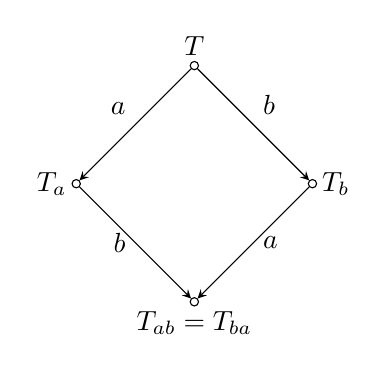
\begin{tikzpicture}[>=stealth]
  % nodes
  \node[circle,draw,inner sep=1pt,minimum size=3pt] (T) at (0,0) {};
  \node[circle,draw,inner sep=1pt,minimum size=3pt] (Ta)
    at (-1.5,-1.5) {};
  \node[circle,draw,inner sep=1pt,minimum size=3pt] (Tb)
    at (1.5,-1.5) {};
  \node[circle,draw,inner sep=1pt,minimum size=3pt] (Tab)
    at (0,-3) {};

  % labels
  \node[above] at (T) {$T$};
  \node[left] at (Ta) {$T_a$};
  \node[right] at (Tb) {$T_b$};
  \node[below] at (Tab) {$T_{ab}=T_{ba}$};

  % arrows
  \draw[->] (T) -- node[above left] {$a$} (Ta);
  \draw[->] (T) -- node[above right] {$b$} (Tb);
  \draw[->] (Ta) -- node[left] {$b$} (Tab);
  \draw[->] (Tb) -- node[right] {$a$} (Tab);
\end{tikzpicture}

  \caption{Local diamond for commuting disjoint updates. Starting from a common
  state $T$, two spacelike-separated reductions $a$ and $b$ can be applied in
  either order, yielding intermediate states $T_a$ and $T_b$ but the same final
  state $T_{ab}=T_{ba}$. The two intermediate events are spacelike-separated:
  they share a common past ($T$) and a common future ($T_{ab}$) but no causal edge
  between them. This expresses a microcausality analogue on the Catalan substrate:
  local updates supported on disjoint subtrees commute and differ only by temporal
  ordering.}
  \label{fig:disjoint-subtrees}
\end{figure}

Lemma~\ref{lem:causal-consistency} states (and sketches a proof of) the
corresponding disjoint-commutation property.

\subsection{Collapse and selection}
Both computation and amplitude propagation require selection:
\begin{itemize}
	\item computational reduction chooses a redex,
	\item measurement-like selection chooses an observable outcome, corresponding
		to an equivalence class under the chosen projection.
\end{itemize}
In the Catalan substrate, selection operates locally, refining rather than
destroying structure. The global constraint ensures consistency after
selection. The formal development of collapse probabilities lies beyond the
scope of this paper and is treated here only structurally.

\subsection{Summary}
Locality and disjoint commutation emerge directly from the causal and recursive
structure of the Catalan lattice. The same principles underlie both
computational reduction and amplitude constructions on the Catalan
history space.

\section{Discussion and Limitations}
\label{sec:discussion}

The results presented here develop a shared structural framework for causal
geometry, a minimal amplitude calculus, and computation. The paper fixes the
Catalan kinematics and makes explicit how amplitudes and computation can be
layered by pair-local constructions (see the scope contract in the
Introduction). The remaining task is to select and calibrate physically
preferred dynamics, in particular interactions/constants and selection rules.

The unification demonstrated here is structural: causal growth, amplitude
propagation (under a chosen phase/readout model), and computation are all
expressible on a common combinatorial substrate. Deriving and calibrating
physically preferred dynamics remains open.

\subsection{Relation to discrete quantum gravity}

Similar scaling behavior appears in two-dimensional quantum gravity and random
surface models. In particular, Causal Dynamical Triangulations (CDT) enforce a
preferred foliation and causal constraint that parallels the prefix order of
Dyck paths \cite{ambjorn01,ambjorn12}. In CDT, the continuum limit is taken
after summing over causally admissible triangulations. Here the admissible
structures are Dyck paths rather than triangulations, but the organizing
principle---the restriction to histories that respect a causal growth rule---is
closely analogous.

\section{Conclusion}
\label{sec:conclusion}

This paper treats the Catalan family (Dyck paths, full binary trees, and
balanced parentheses) as a single discrete history space supporting
three complementary readings: causal geometry via the prefix order, computation
via application trees and local rewrites, and amplitudes via coherent summation
over coarse-grained outcomes. Classical scaling results for conditioned walks
provide a continuum comparison in which Dyck ensembles converge to Brownian
excursions. The underlying diffusion term is governed by the heat operator on
the half-line (with the excursion conditioning represented via a Doob transform),
and under analytic continuation one obtains the free Schr\"odinger equation. The
scope is intentionally restricted to this shared structural core:
deriving interactions, constants, or a unique collapse/measurement rule requires
additional structure beyond what is developed here.

\paragraph{Technical contributions.}
The main technical ingredients include: (i) a classification of pair-local
additive phase functionals and explicit transfer recursions for the Dyck area
phase (Proposition~\ref{prop:phase-classification},
Lemma~\ref{lem:area-transfer}, and
Corollary~\ref{cor:q-catalan-continued-fraction}); (ii) ballot-number completion
formulas and cone self-similarity underlying tier growth
(Lemma~\ref{lem:ballot-completions} and Lemma~\ref{lem:cone-iso-height}); and
(iii) disjoint commutation and the resulting gauge-equivalence viewpoint for
local rewrites (Lemma~\ref{lem:causal-consistency} and
Section~\ref{sec:locality}).

\paragraph{Physics-facing open directions.}
The minimal constructions here suggest several directions for
physics-oriented refinement:
\begin{itemize}
  \item identify principled phase/action functionals (beyond Dyck area) and
    corresponding interaction/potential terms compatible with the pair-local
    dynamics;
  \item clarify the relation between discrete cone coordinates and Lorentzian
    geometry in scaling limits (effective metrics, approximate symmetries, and
    higher-dimensional generalizations);
  \item specify measurement/readout maps and selection rules, and characterize
    which choices reproduce standard quantum statistics beyond toy examples.
\end{itemize}

\appendix

\section{Coordinate Charts and Continuum Comparisons}
\label{appendix:coordinate-charts}

This appendix collects optional coordinate embeddings and continuum comparisons
used for intuition; the combinatorial results in the main text do not depend on
these constructions.

\subsection{Coordinate charts on the Catalan cone}
\label{sec:coordinate-charts}

\begin{remark}[Notation hygiene]
\label{rem:notation-hygiene}
Throughout, the \emph{tier} (semilength) of a completed history is denoted by
$n$, and a \emph{step index} (prefix length) is denoted by
$k\in\{0,1,\dots,2n\}$. Within this subsection, the symbols $(t_k,x_k)$ denote
the embedded coordinates derived from cumulative counts
(Definition~\ref{def:null-counts}); when comparing to continuum formulas we also
write $(t,x)$ for real coordinates.
\end{remark}

\paragraph{The Catalan cone as the master object.}
Let $\mathcal{C}$ denote the set of Dyck prefixes (balanced-parentheses
\emph{prefixes} that never go below height $0$), partially ordered by extension:
$p\preceq q$ iff $q$ has prefix $p$. A completed history is a maximal element
$w\in\mathcal{D}_n\subset\mathcal{C}$ of semilength $n$.
For any prefix $p\in\mathcal{C}$, the future
\[
\mathcal{C}(p)\;:=\;\{\,q\in\mathcal{C}: p\preceq q\,\}
\]
is canonically a ``local cone'' rooted at $p$: the same growth law, re-centered.
Thus there is a single substrate $\mathcal{C}$ (and its re-rootings), and
different ``cones'' arise from different coordinate charts or coarse-grainings
of this same object.

\paragraph{Two cumulative counts and a light-cone chart.}
The most rigid chart on $\mathcal{C}$ is obtained by tracking the cumulative
numbers of opens and closes.

\begin{definition}[Null counts and embedded coordinates]
\label{def:null-counts}
Fix a Dyck word $w\in\mathcal{D}_n$, and let $w[1\!:\!k]$ denote its length-$k$
prefix. Define
\[
u(k)\;:=\;\#\{\texttt{(}\text{ in }w[1\!:\!k]\},\qquad
v(k)\;:=\;\#\{\texttt{)}\text{ in }w[1\!:\!k]\}.
\]
Equivalently, writing $w=w_1\cdots w_{2n}$,
\[
u(k)=\sum_{j=1}^k \mathbf{1}\{w_j=\texttt{(}\},\qquad
v(k)=\sum_{j=1}^k \mathbf{1}\{w_j=\texttt{)}\},
\]
so $(u(k),v(k))$ evolves by unit steps and is step-additive along the prefix.
The Dyck admissibility constraint is $u(k)\ge v(k)$ for all $k$, and completion
is $u(2n)=v(2n)=n$. Define the height (frontier) process
\[
H(k)\;:=\;u(k)-v(k)\;\ge\;0,
\]
and the embedded ``spacetime'' coordinates
\[
t_k\;:=\;\frac{u(k)+v(k)}{2}\;=\;\frac{k}{2},\qquad
x_k\;:=\;\frac{u(k)-v(k)}{2}\;=\;\frac{H(k)}{2}.
\]
Equivalently $u=t_k+x_k$ and $v=t_k-x_k$ (a discrete null-coordinate form).
\end{definition}

Under this embedding, each symbol advances time and changes space by one unit
(up to the $1/2$ normalization):
\[
\texttt{(}:\ (t,x)\mapsto (t+\tfrac12,\ x+\tfrac12),\qquad
\texttt{)}:\ (t,x)\mapsto (t+\tfrac12,\ x-\tfrac12).
\]
Hence the path stays inside the cone $|x_k|\le t_k$, with the boundary $x_k=0$
representing zero frontier (no outstanding opens).

\paragraph{Why ``return to $0$'' is not ``return to the origin.''}
The completion constraint $H(2n)=0$ means only that the \emph{imbalance} vanishes:
every open has been matched by a close. In spacetime coordinates, the endpoint is
\[
(t_{2n},x_{2n})\;=\;\bigl(n,0\bigr),
\]
not $(0,0)$. Thus a history expands monotonically in $t$ (prefix length grows),
while the spatial coordinate $x$ is a \emph{frontier variable} that eventually
returns to $0$ because no unfinished structure may remain at completion.

\paragraph{Pairs, trees, and $S$-expressions are identical structure.}
A Dyck word $w$ can be read as a parenthesized $S$-expression skeleton, and it
already \emph{is} a rooted ordered tree:
matched pairs of parentheses are nodes; containment defines parent/child; and
left-to-right order in the string gives sibling order.
For example, $w=\texttt{(()())}$ has one outer pair (the root) containing two
inner pairs (two leaves). Under this identification, the height $H(k)$ is the
number of currently-open pairs---the size of the \emph{active frontier} of the
tree under construction.

\paragraph{Evaluation ``return'' as frontier discharge.}
If evaluation is recorded at the level of control (continuations), then entering
a subproblem pushes a context frame and finishing it pops that frame. In a
well-bracketed evaluation regime, this push/pop trace is Dyck, and the same
counts $(u(k),v(k))$ track control events. The embedded coordinate $x_k$
therefore measures continuation depth (pending contexts), and the return to
$x=0$ at termination is the emptying of the continuation stack: no pending
contexts remain. Value return is mediated by this control return; the Dyck
``return'' is fundamentally the discharge of outstanding obligations.

\paragraph{Breadth as a different projection (history-level, not frontier-level).}
Statistics such as breadth $b(w)$ summarize a \emph{completed} history by the
maximum size of a constant-depth slice in its associated tree. This is a
coarse-graining of $w$ (many distinct histories share the same $(n,b)$), and it
should be distinguished from the frontier coordinate $x_k$, which is an
instantaneous depth/obligation variable along a single prefix trajectory.

\paragraph{Summary of the two readings.}
There is one substrate $\mathcal{C}$ (and its re-rooted futures $\mathcal{C}(p)$).
Two useful ``cone'' pictures arise from:
(i) the embedded prefix trajectory $(t_k,x_k)$ derived from null counts
(pathwise frontier dynamics), and
(ii) history-level projections such as $(n,b(w))$ (coarse geometric envelope).
The pairs/tree/$S$-expression view does not introduce a new object; it is an
identity of representations of the same Catalan structure.

\subsection{Dyck Coordinates, Lorentz Geometry, and Computational Proper Time}
\label{subsec:dyck-lorentz-computation}

\begin{remark}[Indices and coordinate conventions]
Throughout, $n$ denotes the tier (semilength) of a completed Dyck history.
Within this subsection, $k\in\{0,1,\dots,2n\}$ denotes a \emph{step index} along a
single history, and $m$ denotes the number of \emph{collapse events} (local redex
contractions) performed by a chosen evaluation strategy.
\end{remark}

A Dyck history $w\in\mathcal D_n$ induces the height process $H(k)$ of
Definition~\ref{def:null-counts}. The corresponding embedded coordinates are
$t_k=k/2$ and $x_k=H(k)/2$, so that each parenthesis advances time by $\tfrac12$
and changes the transverse coordinate by $\pm\tfrac12$:
\[
\texttt{(}:\ (t,x)\mapsto (t+\tfrac12,\ x+\tfrac12),\qquad
\texttt{)}:\ (t,x)\mapsto (t+\tfrac12,\ x-\tfrac12).
\]
For any walk with steps $(\Delta t,\Delta x)=(\tfrac12,\pm\tfrac12)$ one has the
kinematic cone bound $|x_k-x_0|\le t_k-t_0$. In the Dyck case, the additional
constraint is one-sided: $x_k\ge 0$ for all $k$, together with the endpoint
condition $x_{2n}=0$. Thus Dyck histories occupy the right half of a discrete
light cone and return to the axis only at completion.

Introduce discrete null coordinates (compare Definition~\ref{def:null-counts})
\[
u:=t+x,\qquad v:=t-x.
\]
In continuum $(1+1)$-dimensional Minkowski space, a Lorentz boost with rapidity
$\eta$ acts linearly as
\begin{equation}
u' = e^{\eta} u,\qquad v' = e^{-\eta} v,
\label{eq:lightcone-boost}
\end{equation}
and transforming back to $(t,x)$ yields the standard Lorentz transformation
\begin{equation}
t' = \gamma (t - v_{\!L} x),\qquad x' = \gamma (x - v_{\!L} t),
\label{eq:lorentz-tx}
\end{equation}
where
\[
\gamma=\frac{1}{\sqrt{1-v_{\!L}^2}},\qquad v_{\!L}=\tanh\eta,
\]
in units $c=1$. The Minkowski interval
\begin{equation}
\mathrm{d}s^{2}=\mathrm{d}t^{2}-\mathrm{d}x^{2}
\label{eq:minkowski}
\end{equation}
is invariant under~\eqref{eq:lorentz-tx}. In this sense the step rule supplies a
discrete null-step kinematics, while the Dyck constraint supplies the boundary
and return conditions selecting the Catalan ensemble. We emphasize that generic
nontrivial boosts do not preserve the discrete Dyck lattice itself (the counts
$u,v$ are integers), so the Lorentz discussion here is a continuum comparison
for the embedded coordinates rather than a discrete symmetry claim.

\begin{remark}[No nontrivial boost preserves the Dyck lattice]
\label{rem:no-lattice-boost}
In the embedded chart, $u$ and $v$ are integer-valued null counts. A Lorentz
boost acts by $(u,v)\mapsto (e^{\eta}u,e^{-\eta}v)$ as in
Equation~\eqref{eq:lightcone-boost}. If such a boost maps $\mathbb Z^2$ to itself,
then $e^{\eta}$ and $e^{-\eta}$ must both be integers, hence
$e^{\eta}e^{-\eta}=1$ forces $e^{\eta}=1$ and $\eta=0$. Thus there is no exact
discrete boost invariance of the integer lattice of null counts (beyond the
identity; discrete reflections correspond to separate, non-boost symmetries).
\end{remark}

\paragraph{Computational proper time.}
A reduction history carries an intrinsic progress parameter given by the count
of collapse events. Let $m$ be the number of local redex contractions performed
by an evaluation strategy up to a given stage, and define the \emph{computational
proper time}
\begin{equation}
\tau := \alpha\, m,
\label{eq:tau-discrete}
\end{equation}
where $\alpha>0$ is the characteristic scale associated with a single collapse.
In continuum Minkowski space, a parametrized world-line $(t(s),x(s))$ admits a
proper-time functional
\begin{equation}
\left(\frac{\mathrm{d}\tau}{\mathrm{d}s}\right)^{2}
=
\left(\frac{\mathrm{d}t}{\mathrm{d}s}\right)^{2}
-
\left(\frac{\mathrm{d}x}{\mathrm{d}s}\right)^{2},
\label{eq:proper-time-continuum}
\end{equation}
which is Lorentz-invariant under~\eqref{eq:lorentz-tx}. In the present discrete
setting, Equation~\eqref{eq:tau-discrete} is simply a well-defined event-count
parameter; the analogy is that collapse count plays the role of a proper-time
progress variable along a chosen computational history.

\subsection{Projection to Height Dynamics and Correlation Structure}
\label{subsec:projection-correlation}

Let $\mathcal{C}$ denote the set of Dyck prefixes, i.e.\ finite words in
$\{(,)\}$ whose height never falls below zero. Each prefix
$p \in \mathcal{C}$ has an associated height
$h(p) \in \mathbb Z_{\ge 0}$ given by the net excess of opening over closing
parentheses. Completed Dyck words of semilength $n$ form the subset
$\mathcal D_n \subset \mathcal{C}$ of prefixes of length $2n$ with
$h=0$.

The Catalan growth rule specifies admissible extensions: from a prefix $p$,
one may append ``$(\,$'' unconditionally, or ``$)\,$'' provided $h(p)>0$.
To describe this probabilistically, it is convenient to separate the base
process from the Dyck-conditioned ensemble.

\paragraph{Base height process.}
Let $(H_t)_{t\ge0}$ be a simple symmetric random walk on $\mathbb Z$ with
increments $\pm1$. This walk is time-homogeneous and Markov. Its sample paths
may be viewed as unconstrained height sequences, without regard to the Dyck
condition.

\paragraph{Dyck conditioning.}
The Dyck ensemble of length $T=2n$ is obtained by conditioning the base walk on
the event
\[
\{ H_t \ge 0 \text{ for all } t \le T,\; H_T = 0 \}.
\]
Under this conditioning, the law of $(H_t)_{t=0}^T$ is uniform on Dyck paths of
semilength $n$. Equivalently, the conditioned process may be represented via a
Doob $h$-transform (or bridge kernel) of the base walk. In this representation,
the height process remains Markov but becomes time-inhomogeneous due to the
global conditioning. Each completed Dyck word
$p \in \mathcal D_n$ corresponds uniquely to a sample path
\[
(h_0,h_1,\dots,h_T), \qquad h_0=h_T=0,\; h_t\ge0,
\]
drawn from this conditioned law.

\begin{lemma}[Conditioned transition probabilities]
\label{lem:dyck-conditioned-kernel}
For integers $r\ge 0$ and $h\ge 0$, let $B(r,h)$ denote the number of
nonnegative $\pm 1$ paths of length $r$ that start at height $h$ and end at $0$
(so $B(r,h)=0$ unless $r\ge h$ and $r\equiv h\ (\mathrm{mod}\ 2)$). Then the Dyck
conditioning above yields a time-inhomogeneous Markov chain. Writing
\[
\mathcal{E}:=\{H_s\ge 0\text{ for all }s\le T,\; H_T=0\},
\]
its one-step transition probabilities are, for $0\le t<T$ and $h\ge 0$ with
$B(T-t,h)>0$,
\[
\mathbb P(H_{t+1}=h+1 \mid H_t=h,\; \mathcal{E})
\;=\;
\frac{B(T-t-1,h+1)}{B(T-t,h)},
\]
\[
\mathbb P(H_{t+1}=h-1 \mid H_t=h,\; \mathcal{E})
\;=\;
\frac{B(T-t-1,h-1)}{B(T-t,h)},
\]
with the convention $B(\cdot,-1)=0$ (so the down-step probability is $0$ at
$h=0$). Moreover, $B(r,h)$ is given explicitly by the ballot-number formula of
Lemma~\ref{lem:ballot-completions} (taking $r$ as the remaining step budget).
\end{lemma}

\begin{remark}[Closed form]
\label{rem:dyck-conditioned-kernel-closed}
Writing $r:=T-t$ and assuming $B(r,h)>0$, Lemma~\ref{lem:ballot-completions}
gives the explicit probabilities
\[
\mathbb P(H_{t+1}=h+1 \mid H_t=h,\; \mathcal{E})
=\frac{(h+2)(r-h)}{2r(h+1)},
\qquad
\mathbb P(H_{t+1}=h-1 \mid H_t=h,\; \mathcal{E})
=\frac{h(r+h+2)}{2r(h+1)}.
\]
In particular, the conditional drift is
\[
\mathbb E[H_{t+1}-H_t \mid H_t=h,\; \mathcal{E}]
=\frac{r-h(h+2)}{r(h+1)}.
\]
\end{remark}

\begin{remark}[Drift scaling and the Bessel-bridge limit]
\label{rem:dyck-conditioned-drift-scaling}
Fix semilength $n$ so that $T=2n$. Consider the rescaled time parameter
$\tau:=t/n\in[0,2]$ and the rescaled height $X^{(n)}(\tau):=n^{-1/2}H_{\lfloor n\tau\rfloor}$.
If $H_t$ is of order $\sqrt{n}$, write $h=\lfloor \sqrt{n}\,x\rfloor$ and note that
$r=T-t\approx n(2-\tau)$. Substituting into the exact drift formula in
Remark~\ref{rem:dyck-conditioned-kernel-closed} gives the formal approximation
\[
\mathbb E\!\left[X^{(n)}\!\left(\tau+\tfrac1n\right)-X^{(n)}(\tau)\mid X^{(n)}(\tau)\approx x,\ \mathcal E\right]
\approx \frac{1}{n}\left(\frac{1}{x}-\frac{x}{2-\tau}\right),
\]
exhibiting a repulsive term $1/x$ from the hard wall at $0$ together with an
attractive term $-x/(2-\tau)$ enforcing return to $0$ at time horizon $2$.
This matches the time-inhomogeneous drift of the $3$-dimensional Bessel bridge
representation of Brownian excursion \cite{pitman1999,takacs1991}.
\par
More explicitly, a $3$-dimensional Bessel bridge $(X_\tau)_{0\le \tau <2}$ from
$0$ to $0$ over time horizon $2$ solves the SDE
\[
\mathrm{d}X_\tau
= \mathrm{d}B_\tau
\;+\;\left(\frac{1}{X_\tau}-\frac{X_\tau}{2-\tau}\right)\mathrm{d}\tau,
\]
where the singular drift $1/X_\tau$ encodes conditioning to stay nonnegative and
the term $-X_\tau/(2-\tau)$ encodes the bridge-to-$0$ constraint.
\end{remark}

\begin{remark}[Doob transform and completion weighting]
\label{rem:dyck-conditioned-kernel-doob}
Let $P$ be the kernel of the simple symmetric walk killed upon attempting to step
from $0$ to $-1$. Equivalently, adjoin a cemetery state $\dagger$ and take
$P(0,1)=P(0,\dagger)=1/2$ and $P(h,h\pm 1)=1/2$ for $h>0$, then restrict to
$\mathbb Z_{\ge 0}$ (so $P$ is sub-Markov at $0$).
Writing again $r:=T-t$, the function $h_r(h):=B(r,h)$ is the number of admissible
completions from height $h$ in $r$ remaining steps and satisfies the backward
recursion of Lemma~\ref{lem:ballot-recurrence}. The conditioned chain in
Lemma~\ref{lem:dyck-conditioned-kernel} is exactly the time-inhomogeneous Doob
$h$-transform of $P$ with $h_r$:
\[
\mathbb P(H_{t+1}=h\pm 1 \mid H_t=h,\; \mathcal{E})
= P(h,h\pm 1)\,\frac{h_{r-1}(h\pm 1)}{h_r(h)}
= \frac{B(r-1,h\pm 1)}{B(r,h)},
\]
so the next step is chosen with probability proportional to the number of
admissible futures after taking that step.
\end{remark}

\begin{proof}[Proof sketch]
Because the base walk is simple symmetric, all length-$T$ paths have equal
probability $2^{-T}$, so conditioning yields the uniform distribution on
admissible paths. Given $H_t=h$, the conditional probability of an up step is
proportional to the number of admissible completions from height $h+1$ in the
remaining $T-t-1$ steps, and similarly for a down step; normalizing gives the
stated ratios. The explicit binomial difference for $B(r,h)$ follows from the
reflection principle / ballot theorem \cite{stanley-catalan}.
\end{proof}

\begin{lemma}[Recurrence for completion counts]
\label{lem:ballot-recurrence}
The completion counts $B(r,h)$ satisfy
\[
B(0,0)=1,\qquad B(0,h)=0\ \text{for }h>0,
\]
and for $r\ge 1$ and $h\ge 0$,
\[
B(r,h)=B(r-1,h-1)+B(r-1,h+1),
\]
with the convention $B(r,-1):=0$.
\end{lemma}

\begin{proof}
Decompose a nonnegative length-$r$ path from height $h$ to $0$ by its first
step. After a down step (to $h-1$) or up step (to $h+1$), there remain $r-1$
steps to reach $0$ without crossing below $0$. Summing these disjoint cases
gives the recurrence; the boundary convention $B(r,-1)=0$ enforces the
nonnegativity constraint.
\end{proof}

\begin{lemma}[Catalan-triangle height marginal]
\label{lem:height-marginal}
Let $T=2n$ and consider the uniform measure on Dyck paths of semilength $n$.
For $0\le t\le T$ and $h\ge 0$, the number of Dyck paths with $H_t=h$ factors as
\[
\#\{w\in\mathcal D_n : H_w(t)=h\}
= B(t,h)\,B(T-t,h),
\]
and hence
\[
\mathbb P(H_t=h)=\frac{B(t,h)\,B(T-t,h)}{C_n},
\qquad C_n=B(T,0).
\]
\end{lemma}

\begin{proof}[Proof sketch]
Split a Dyck path at time $t$. The prefix from $0$ to $h$ of length $t$ and the
suffix from $h$ to $0$ of length $T-t$ must both stay nonnegative. By time
reversal, the number of admissible prefixes from $0$ to $h$ of length $t$ equals
$B(t,h)$, and admissible suffixes are counted by $B(T-t,h)$. Concatenating a
prefix and suffix yields a Dyck path with $H_t=h$, and this factorization is
bijective.
\end{proof}

\begin{definition}[Nonnegative bridge counts]
\label{def:nonnegative-bridge}
For $r\ge 0$ and $a,b\in\mathbb Z_{\ge 0}$, write $B(r; a\!\to\! b)$ for the
number of length-$r$ $\pm 1$ paths that start at height $a$, end at height $b$,
and remain nonnegative throughout. In particular, the completion counts in
Lemma~\ref{lem:dyck-conditioned-kernel} are $B(r,h)=B(r;h\!\to\!0)$.
\end{definition}

\begin{lemma}[Ballot-number bridge count]
\label{lem:ballot-bridge}
For $r\ge 0$ and $a,b\in\mathbb Z_{\ge 0}$,
\[
B(r; a\!\to\! b)
=
\binom{r}{\frac{r+b-a}{2}}
\;-\;
\binom{r}{\frac{r+b+a}{2}+1},
\]
with the convention $\binom{r}{k}=0$ when $k\notin\{0,1,\dots,r\}$ or $k$ is not
an integer. In particular, $B(r,h)=B(r;h\!\to\!0)$ agrees with the completion
count of Lemma~\ref{lem:ballot-completions}.
\end{lemma}

\begin{proof}[Proof sketch]
Count all length-$r$ $\pm 1$ paths from $a$ to $b$ and subtract those that ever
hit $-1$. Reflect the initial segment up to the first visit to $-1$; this gives
a bijection between paths from $a$ to $b$ that hit $-1$ and unconstrained paths
from $-a-2$ to $b$. Evaluating both counts yields the stated binomial difference;
see \cite{stanley-catalan}.
\end{proof}

\begin{lemma}[Two-time height marginal]
\label{lem:two-time-height-marginal}
Let $T=2n$ and consider the uniform measure on Dyck paths of semilength $n$.
For $0\le s\le t\le T$ and $a,b\ge 0$, the number of Dyck paths with
$H_s=a$ and $H_t=b$ factors as
\[
\#\{w\in\mathcal D_n : H_w(s)=a,\ H_w(t)=b\}
= B(s;0\!\to\!a)\,B(t-s;a\!\to\!b)\,B(T-t;b\!\to\!0),
\]
and hence
\[
\mathbb P(H_s=a,\ H_t=b)
=\frac{B(s;0\!\to\!a)\,B(t-s;a\!\to\!b)\,B(T-t;b\!\to\!0)}{C_n},
\qquad C_n=B(T;0\!\to\!0).
\]
\end{lemma}

\begin{proof}[Proof sketch]
Split a Dyck path into three segments: from time $0$ to $s$ (height $0\to a$),
from $s$ to $t$ (height $a\to b$), and from $t$ to $T$ (height $b\to 0$). The
Dyck constraint implies that each segment stays nonnegative, so concatenation
gives a bijection between Dyck paths realizing $(H_s,H_t)=(a,b)$ and triples of
nonnegative segments counted by the product above.
\end{proof}

\begin{lemma}[Multi-time factorization and Markov kernel]
\label{lem:multi-time-factorization}
Let $T=2n$ and consider the uniform measure on Dyck paths of semilength $n$.
Fix times $0=t_0\le t_1\le \cdots \le t_m\le T$ and heights
$h_0:=0,h_1,\dots,h_m\in\mathbb Z_{\ge 0}$. Then
\[
\#\{w\in\mathcal D_n : H_w(t_j)=h_j\ \text{for all }j=1,\dots,m\}
=
\Big(\prod_{j=1}^m B(t_j-t_{j-1}; h_{j-1}\!\to\! h_j)\Big)\,B(T-t_m;h_m\!\to\!0).
\]
In particular, $(H_t)_{0\le t\le T}$ under the uniform Dyck measure is a
time-inhomogeneous Markov chain on $\mathbb Z_{\ge 0}$ with transition
probabilities, for $0\le s\le t\le T$,
\[
\mathbb P(H_t=b \mid H_s=a)
=
\frac{B(t-s; a\!\to\! b)\,B(T-t; b\!\to\! 0)}{B(T-s; a\!\to\! 0)},
\]
whenever $B(T-s;a\!\to\!0)>0$.
\end{lemma}

\begin{proof}[Proof sketch]
Split a Dyck path into consecutive nonnegative bridge segments between the
prescribed times; concatenation is bijective and multiplies counts. The Markov
kernel follows by dividing the two-time count by the one-time marginal
(Lemma~\ref{lem:height-marginal}).
\end{proof}

\paragraph{Correlation structure.}
Consider the ensemble of height paths of fixed length $T$, distributed
according to the Dyck-conditioned law. Define the mean and covariance functions
\[
\mu_t := \mathbb E[H_t], \qquad
C(s,t) := \mathbb E\!\left[(H_s-\mu_s)(H_t-\mu_t)\right],
\qquad 0\le s,t\le T .
\]
\begin{remark}[Explicit mean and covariance formulas]
By Lemma~\ref{lem:height-marginal},
\[
\mu_t
=\sum_{h\ge 0} h\,\frac{B(t,h)\,B(T-t,h)}{C_n}.
\]
By Lemma~\ref{lem:two-time-height-marginal},
\[
\mathbb E[H_s H_t]
=\sum_{a,b\ge 0} a b\,
\frac{B(s;0\!\to\! a)\,B(t-s;a\!\to\! b)\,B(T-t;b\!\to\! 0)}{C_n},
\]
and hence $C(s,t)=\mathbb E[H_s H_t]-\mu_s\mu_t$.
All bridge counts $B(\cdot;\cdot\!\to\!\cdot)$ admit explicit binomial
expressions by Lemma~\ref{lem:ballot-bridge}.
\end{remark}
The covariance kernel $C$ is a symmetric positive operator on the finite-dimensional
space $\mathbb R^{T+1}$ and captures the second-order temporal structure induced
by the Dyck constraint. It admits an eigen-decomposition
\[
\sum_{t=0}^{T} C(s,t)\,v^{(k)}_t = \lambda_k\, v^{(k)}_s ,
\]
yielding an orthogonal family of temporal modes. Any centered height profile
admits the expansion
\[
H_t-\mu_t = \sum_k \xi_k\, v^{(k)}_t ,
\qquad \mathbb E[\xi_k\xi_\ell]=\lambda_k\,\delta_{k\ell}.
\]
In this precise sense, the eigenvalues $\lambda_k$ constitute the spectrum of
temporal correlations induced by the Dyck-conditioned dynamics, and the
associated eigenvectors provide a canonical modal decomposition
(Karhunen--Lo\`eve expansion) of Dyck height signals.

\paragraph{Scaling limit.}
Under diffusive scaling, the base random walk converges to Brownian motion on
$\mathbb R$. The Dyck-conditioned law converges to Brownian excursion, which may
be described equivalently as Brownian motion conditioned to remain nonnegative
and return to zero, or via a Doob transform / Bessel-bridge representation
\cite{takacs1991,pitman1999} (compare Remark~\ref{rem:dyck-conditioned-drift-scaling}).
The resulting continuum evolution is governed by a
second-order differential operator on $\mathbb R_{\ge0}$ whose drift and boundary
behavior encode the conditioning. In related unconditioned or bridge settings,
the associated covariance eigenfunctions are explicitly sinusoidal; for the
excursion case, the exact eigenstructure is more subtle, though the dominant
modes often resemble sine-like functions away from boundaries.

Thus, the appearance of modal structure follows directly from the projection of
Catalan growth dynamics to the height observable and the standard spectral
analysis of the resulting correlation kernel, without the introduction of
additional postulates beyond the Dyck-conditioned height process and standard
spectral analysis.

\begin{remark}[Self-similarity and reference frames]
The Dyck prefix structure is recursively self-similar: every prefix is itself
the root of a complete Catalan subtree. Consequently, distinctions such as
parent and child, past and future, or global and local history are not
intrinsic to the substrate but arise only after fixing a reference root, which
induces a causal orientation. The projected height dynamics, their conditioning,
and their scaling limits are invariant under such re-rootings.
\end{remark}


\section{A Double-Slit Thought Experiment on the Catalan Light Cone}
\label{appendix:doubleslit}

This appendix provides an illustrative thought experiment showing how the
discrete path-integral formalism developed in Section~\ref{sec:amplitudes}
exhibits interference in a setting analogous to the double-slit experiment.
The construction is entirely combinatorial and finite. No new assumptions,
dynamical rules, or continuum limits are introduced; the purpose is solely to
instantiate the formalism in a familiar narrative.
Throughout, we take the phase functional to be the Dyck area $A(w)$ introduced
in Section~\ref{sec:amplitudes}, i.e.\ $\psi(w)=e^{i\alpha A(w)}$ (a special
case of Proposition~\ref{prop:phase-classification}).

\subsection{Two sources as boundary-conditioned cones}

Consider two distinct Dyck prefixes $u_L$ and $u_R$ of equal length and height.
Each prefix induces a local Catalan cone of admissible continuations, as
described in Section~\ref{sec:multiplecones}. We refer to these as the left and
right source cones, although no spatial interpretation is assumed at this
stage.

Both cones are evolved to a common tier $n$, producing two ensembles of Dyck
paths of semilength $n$ that differ only in their initial boundary condition.
The admissible histories from both cones are evaluated relative to the same
observable defined below.

\subsection{Observable and indistinguishability}

Fix a tier $n$ and define an observable
\[
f : \mathcal D_n \to \mathcal X,
\]
where $\mathcal X$ is a discrete outcome space. The observable $f$ retains a
coarse-grained feature of each history (for example, a bin determined by the
mean height or total area) and discards all other information, including which
source cone the history originated from.

Interference arises precisely because histories originating from distinct cones
may be rendered indistinguishable by the observable. If the observable were to
retain source information, no interference would occur.

\subsection{A worked finite example}
\label{subsec:doubleslit-worked}

Take $n=4$ and choose two admissible Dyck prefixes of equal length and height,
\[
u_L=\texttt{(()(}, \qquad u_R=\texttt{()((},
\]
each of length $4$ and height $2$. Each prefix admits exactly three completions
to a full Dyck word of length $8$, yielding six histories in the union of the
two source cones.

Define a coarse observable that discards source information by sampling the
height at a fixed time step after the ``slits'':
\[
f(w) := H_w(6)\in\{0,2\}.
\]
	This is a discrete analogue of recording transverse displacement at a detector
	time without access to which slit was taken.
	The areas $A(w)$ listed below are computed directly from
	Lemma~\ref{lem:area-pair-lifetimes}; we list them without further derivation.

\begin{table}[ht]
\centering
\begin{tabular}{llll}
\hline
cone & $w$ & $A(w)$ & $f(w)=H_w(6)$ \\
\hline
$L$ & \texttt{(()(()))} & $12$ & $2$ \\
$L$ & \texttt{(()()())} & $10$ & $2$ \\
$L$ & \texttt{(()())()} & $8$  & $0$ \\
$R$ & \texttt{()((()))} & $10$ & $2$ \\
$R$ & \texttt{()(()())} & $8$  & $2$ \\
$R$ & \texttt{()(())()} & $6$  & $0$ \\
\hline
\end{tabular}
\caption{Two equal-height source cones at $n=4$ and a coarse detector observable.}
\end{table}

With phase $\psi(w)=e^{i\alpha A(w)}$, the detector amplitudes are
\[
\Psi(2)=\sum_{f(w)=2} e^{i\alpha A(w)}
= e^{i12\alpha}+2e^{i10\alpha}+e^{i8\alpha}
= 2e^{i10\alpha}\bigl(1+\cos(2\alpha)\bigr),
\]
\[
\Psi(0)=\sum_{f(w)=0} e^{i\alpha A(w)}
= e^{i8\alpha}+e^{i6\alpha}
= 2e^{i7\alpha}\cos(\alpha).
\]
By counting alone one would predict multiplicities $N(2)=4$ and $N(0)=2$. In contrast,
	the Born-style intensities $|\Psi(x)|^2$ vary with $\alpha$ and can exhibit strong
	suppression. For example, at $\alpha=\pi/2$ one obtains $\Psi(2)=0$ (exact
	destructive interference at the outcome $x=2$), even though $N(2)=4$ histories
	contribute.
	This discrepancy between raw multiplicities $N(x)$ and intensities $|\Psi(x)|^2$
	is what we mean by interference in this discrete setting.

This example is intentionally tiny: its purpose is to show, in finite
combinatorial terms, how (i) multiple histories per outcome, (ii) an additive
phase functional, and (iii) coarse observation together produce interference.
Larger $n$ yields richer outcome sets and more intricate cancellation patterns.

\subsection{Summary}
No wave equation, spatial geometry, or continuum approximation is assumed in
this construction. The example simply instantiates the general mechanism of
Section~\ref{sec:amplitudes}: complex weights, coherent summation over
coarse-grained preimages, and Born-style squaring suffice to produce
interference.

\section{A Conditional Uniqueness Theorem for the Dyck-Prefix Substrate}
\label{appendix:uniqueness}

This appendix isolates a minimal set of structural axioms under which the
Dyck-prefix substrate is not merely an example but is determined uniquely up to
isomorphism. The result is interpretation-neutral: it assumes no particular
computational semantics (evaluation order, combinators, rewriting), only a
ranked causal-growth structure with a one-sided admissibility boundary.

\subsection{Ranked growth posets}

\begin{definition}[Ranked growth poset]
\label{def:ranked-growth-poset}
A \emph{ranked growth poset} is a triple $(S,\preceq,\mathrm{rk})$ where $S$ is a
countable set, $\preceq$ is a partial order on $S$, and
$\mathrm{rk}:S\to\mathbb{N}$ is a rank function such that:
\begin{enumerate}[label=(\roman*)]
\item for every $t\in S$ the set $\{s\in S : s\preceq t\}$ is finite, and
\item $\mathrm{rk}$ is strictly order-increasing along cover relations.
\end{enumerate}
Write $s\prec t$ when $s\preceq t$ and $s\neq t$, and write
$s\lessdot t$ if $s\prec t$ and there is no $u$ with $s\prec u\prec t$
(i.e.\ $t$ \emph{covers} $s$).
\end{definition}

\begin{definition}[Two-move height structure]
\label{def:two-move-height}
Let $(S,\preceq,\mathrm{rk})$ be a ranked growth poset with a distinguished root
$s_{\emptyset}\in S$ satisfying $\mathrm{rk}(s_{\emptyset})=0$.
A \emph{two-move height structure} on $S$ consists of a function
$h:S\to\mathbb{Z}_{\ge 0}$ (height) with $h(s_{\emptyset})=0$ such that every
cover relation $s\lessdot t$ satisfies
\[
\mathrm{rk}(t)=\mathrm{rk}(s)+1
\qquad\text{and}\qquad
h(t)=h(s)\pm 1.
\]
We call a cover with $h(t)=h(s)+1$ an \emph{up-step} and a cover with
$h(t)=h(s)-1$ a \emph{down-step}.
\end{definition}

\subsection{Axioms for the Catalan core}

The uniqueness theorem below follows from four axioms capturing: (i) discrete
single-step growth, (ii) exactly two local move types (up/down), (iii) a
one-sided boundary in which down-steps are disabled at height $0$, and (iv) an
\emph{unfolded} (collision-free) history space.

\begin{definition}[Catalan core axioms]
\label{def:catalan-core-axioms}
A ranked growth poset $(S,\preceq,\mathrm{rk})$ with root $s_{\emptyset}$ and
two-move height structure $h$ satisfies the \emph{Catalan core axioms} if:
\begin{enumerate}[label=(A\arabic*)]
\item \textbf{(Ranked single-step growth)} For every cover $s\lessdot t$, one has
$\mathrm{rk}(t)=\mathrm{rk}(s)+1$ and $h(t)=h(s)\pm 1$.

\item \textbf{(Local determinism by move type)} For each $s\in S$, there exists
\emph{at most one} up-step successor $t_{\uparrow}$ with $s\lessdot t_{\uparrow}$
and $h(t_{\uparrow})=h(s)+1$, and \emph{at most one} down-step successor
$t_{\downarrow}$ with $s\lessdot t_{\downarrow}$ and $h(t_{\downarrow})=h(s)-1$.

\item \textbf{(One-sided boundary admissibility)} For each $s\in S$, an up-step
successor exists, while a down-step successor exists \emph{iff} $h(s)>0$.

\item \textbf{(No collisions / unique history)} Each $t\in S$ admits a unique
saturated chain (cover chain) from the root:
\[
s_{\emptyset}=s_0 \lessdot s_1 \lessdot \cdots \lessdot s_{\mathrm{rk}(t)}=t.
\]
\end{enumerate}
\end{definition}

\subsection{Dyck-prefix poset}

Let $\Sigma=\{+,-\}$. For a word $w=w_1\cdots w_n\in\Sigma^n$, define the
partial-sum height
\[
H_w(k)=\sum_{j=1}^k \xi(w_j),
\qquad
\text{where }\xi(+)=+1,\ \xi(-)=-1.
\]
Call $w$ \emph{admissible} if $H_w(k)\ge 0$ for all $k$.
Let $\mathcal{C}$ be the set of all admissible words (Dyck prefixes), partially
ordered by prefix: $u\preceq v$ iff $u$ is a prefix of $v$. Let $\ell(w)=n$ be
length and $H(w)=H_w(n)$ be final height.

\begin{definition}[Dyck-prefix poset]
\label{def:dyck-prefix-poset}
The \emph{Dyck-prefix poset} is $(\mathcal{C},\preceq,\ell)$ with root
$\varepsilon$ (the empty word).
\end{definition}

\subsection{Uniqueness theorem}

\begin{theorem}[Dyck-prefix uniqueness]
\label{thm:dyck-uniqueness}
Let $(S,\preceq,\mathrm{rk})$ be a ranked growth poset with root $s_{\emptyset}$
and a two-move height structure $h$. If $S$ satisfies the Catalan core axioms of
Definition~\ref{def:catalan-core-axioms}, then there exists a unique bijection
\[
\pi:S\to\mathcal{C}
\]
such that for every $s\in S$,
\[
\ell(\pi(s))=\mathrm{rk}(s),
\qquad
H(\pi(s))=h(s),
\]
and $\pi$ is an order isomorphism:
\[
s\preceq t \quad\Longleftrightarrow\quad \pi(s)\preceq \pi(t)
\quad\text{(prefix order).}
\]
In particular, $(S,\preceq,\mathrm{rk})$ is isomorphic to the Dyck-prefix poset.
\end{theorem}

\begin{proof}
By (A4), each $s\in S$ admits a unique cover chain
$s_{\emptyset}=s_0\lessdot\cdots\lessdot s_n=s$ where $n=\mathrm{rk}(s)$. Define
a word $\pi(s)\in\Sigma^n$ by setting
\[
\pi(s)_k=
\begin{cases}
+ & \text{if } h(s_k)=h(s_{k-1})+1,\\
- & \text{if } h(s_k)=h(s_{k-1})-1.
\end{cases}
\]
This is well-defined and has length $\ell(\pi(s))=n$. By construction, the
partial sums of $\pi(s)$ coincide with the height along the chain,
\[
H_{\pi(s)}(k)=h(s_k)\ge 0 \quad\text{for all }k,
\]
so $\pi(s)$ is admissible and $\pi(s)\in\mathcal{C}$. Moreover
$H(\pi(s))=H_{\pi(s)}(n)=h(s)$.

We now show that $\pi$ is bijective. Given any admissible word
$w=w_1\cdots w_n\in\mathcal{C}$, construct a chain in $S$ by starting at
$s_0=s_{\emptyset}$ and for each $k\ge 1$ taking the successor specified by
$w_k$:
\[
s_k=
\begin{cases}
\text{the (unique) up-step successor of } s_{k-1} & \text{if } w_k=+,\\
\text{the (unique) down-step successor of } s_{k-1} & \text{if } w_k=-.
\end{cases}
\]
Existence and uniqueness follow from (A2)--(A3); admissibility of $w$ ensures
that a down-step is only requested when the current height is positive. Let
$s:=s_n$ be the resulting node at rank $n$. Then $\pi(s)=w$, proving
surjectivity. Injectivity follows from (A4): distinct nodes have distinct
cover chains and hence distinct step sequences.

Finally, $\pi$ preserves order. If $s\preceq t$, then the unique chain to $t$
contains the chain to $s$ as an initial segment, so $\pi(s)$ is a prefix of
$\pi(t)$. Conversely, if $\pi(s)$ is a prefix of $\pi(t)$, then the constructed
chain for $\pi(t)$ passes through the constructed chain for $\pi(s)$, giving
$s\preceq t$. Uniqueness of $\pi$ is immediate from (A4), since $\pi(s)$ is
forced by the unique cover chain to~$s$.
\end{proof}

\subsection{Catalan enumeration at completion}

To recover the usual Catalan counting, impose a completion boundary condition:
completion occurs when the height returns to zero at even rank.

\begin{definition}[Completed histories]
\label{def:completed-histories}
For $n\in\mathbb{N}$, define the set of \emph{completed histories} at rank $2n$ by
\[
S^{\mathrm{comp}}_{2n} := \{s\in S : \mathrm{rk}(s)=2n \text{ and } h(s)=0\}.
\]
\end{definition}

\begin{corollary}[Catalan counting]
\label{cor:catalan-counting}
Under the hypotheses of Theorem~\ref{thm:dyck-uniqueness}, the number of
completed histories satisfies
\[
\#\bigl(S^{\mathrm{comp}}_{2n}\bigr)=C_n
=\frac{1}{n+1}\binom{2n}{n},
\]
the $n$th Catalan number.
\end{corollary}

\begin{proof}
By Theorem~\ref{thm:dyck-uniqueness}, $S^{\mathrm{comp}}_{2n}$ is in bijection
with admissible words of length $2n$ with final height $0$, i.e.\ Dyck words of
semilength $n$. These are counted by the Catalan number $C_n$.
\end{proof}

\subsection{Quotients and structural sharing}

The ``no collisions'' axiom (A4) asserts that $S$ is an \emph{unfolded} history
space: each node encodes a distinct growth history. This does not preclude gauge
equivalences or multi-way computation graphs; rather, those arise by quotienting
$S$ by an equivalence relation.

\begin{remark}[Quotients and gauge identification]
\label{rem:gauge-quotient}
Let $\sim$ be an equivalence relation on $S$ representing gauge or rewrite
identifications. The quotient set $S/{\sim}$ may exhibit merges (a DAG-like
state graph), even if $S$ is collision-free. Theorem~\ref{thm:dyck-uniqueness}
characterizes the unfolded core; quotient structure is encoded by the choice of
$\sim$ and acts as an identification of histories rather than a primitive
feature of the substrate.
\end{remark}

\begin{remark}[Structural sharing vs.\ semantic collisions]
\label{rem:sharing}
Axiom (A4) concerns semantic identity in $S$ (distinct histories are distinct
nodes). It is compatible with immutability and structural sharing in
implementations (e.g.\ hash-consing), which may share representation of common
substructures without identifying distinct history nodes.
\end{remark}

\subsection{Scope of the result}

Theorem~\ref{thm:dyck-uniqueness} establishes a core uniqueness statement:
given two local move types changing an integer height by $\pm 1$, a one-sided
boundary disabling down-steps at height $0$, and an unfolded history space, the
substrate is forced to be Dyck-prefix order. This statement is independent of
additional semantic layers (program interpretations, rewriting dynamics, or
amplitude assignments), which can be imposed on top of the substrate without
affecting the isomorphism.

\section{Unfoldings and Covers of Growth Posets}
\label{appendix:unfoldings}

Many natural representations of computation or gauge-identified state spaces
exhibit merges: distinct growth histories may lead to the same state, producing
a DAG-like multi-way graph rather than a tree. The core uniqueness theorem in
Appendix~\ref{appendix:uniqueness} characterizes the \emph{unfolded} history
space. This appendix makes that relationship explicit by defining a canonical
unfolding (history cover) for a ranked growth poset and showing that the Catalan
uniqueness statement applies upstairs even when merges exist downstairs.

\subsection{Growth graphs}

\begin{definition}[Rooted ranked growth poset]
\label{def:rooted-ranked-growth-poset}
A \emph{rooted ranked growth poset} is a ranked growth poset
$(S,\preceq,\mathrm{rk})$ (Definition~\ref{def:ranked-growth-poset}) equipped
with a distinguished root $s_{\emptyset}\in S$ such that for every $s\in S$ one
has $s_{\emptyset}\preceq s$ (i.e.\ every node is reachable from the root).
\end{definition}

\begin{definition}[Directed growth graph]
\label{def:directed-growth-graph}
Let $(S,\preceq,\mathrm{rk})$ be a rooted ranked growth poset.
Its \emph{directed growth graph} is the rooted directed graph
$G(S)=(V,E,s_{\emptyset})$ where $V=S$ and $(s,t)\in E$ iff $s\lessdot t$
(i.e.\ $t$ covers $s$). We regard each edge as a single-step growth move.
\end{definition}

\begin{definition}[Move type induced by height]
\label{def:move-type}
If $(S,\preceq,\mathrm{rk})$ carries a two-move height structure $h$
(Definition~\ref{def:two-move-height}), then each directed edge $s\to t$ in
$G(S)$ has a \emph{move type}
\[
\mathrm{type}(s\to t)\in\{+,-\}
\quad\text{defined by}\quad
\mathrm{type}(s\to t)=
\begin{cases}
+ & \text{if } h(t)=h(s)+1,\\
- & \text{if } h(t)=h(s)-1.
\end{cases}
\]
\end{definition}

\subsection{Rooted covers (local isomorphism in one step)}

To model ``the same local growth rule everywhere'' we use a minimal notion of
cover: a map that is locally bijective on outgoing edges from each node. This
avoids introducing general poset coverings and suffices for the unfolding
argument below.

\begin{definition}[Rooted directed cover]
\label{def:rooted-directed-cover}
Let $G=(V,E,r)$ and $\widetilde{G}=(\widetilde{V},\widetilde{E},\widetilde{r})$
be rooted directed graphs. A function $\varphi:\widetilde{V}\to V$ is a
\emph{rooted directed cover} if:
\begin{enumerate}[label=(\roman*)]
\item $\varphi(\widetilde{r})=r$;
\item for every $\widetilde{v}\in\widetilde{V}$, the map
\[
\varphi_*:\mathrm{Out}(\widetilde{v})\to \mathrm{Out}(\varphi(\widetilde{v})),
\qquad
(\widetilde{v}\to \widetilde{w})\mapsto (\varphi(\widetilde{v})\to \varphi(\widetilde{w}))
\]
is a bijection, where $\mathrm{Out}(x)=\{x\to y\in E\}$ denotes the set of
outgoing edges from $x$.
\end{enumerate}
If edges carry move types $\{+,-\}$, we additionally require that $\varphi_*$
preserves move type (i.e.\ the bijection matches $+$-edges to $+$-edges and
$-$-edges to $-$-edges).
\end{definition}

\subsection{The canonical unfolding (history cover)}

\begin{definition}[Unfolding as rooted path space]
\label{def:unfolding}
Let $(S,\preceq,\mathrm{rk})$ be a rooted ranked growth poset and let $G(S)$ be
its directed growth graph.
Define the \emph{unfolding} $\widetilde{S}$ to be the set of all finite directed
paths in $G(S)$ starting at the root:
\[
\widetilde{S}
:=\bigl\{
(s_0\to s_1\to\cdots\to s_n)\ :\ s_0=s_{\emptyset},\ (s_{k-1},s_k)\in E
\bigr\}.
\]
Write $\widetilde{s}=(s_0\to\cdots\to s_n)$ and define:
\begin{enumerate}[label=(\roman*)]
\item the \emph{endpoint} map $\varphi:\widetilde{S}\to S$ by
$\varphi(\widetilde{s})=s_n$;
\item the \emph{rank} $\widetilde{\mathrm{rk}}(\widetilde{s})=n$ (path length);
\item the \emph{prefix order} on $\widetilde{S}$:
$\widetilde{u}\preceq \widetilde{v}$ iff $\widetilde{u}$ is an initial segment
(prefix) of $\widetilde{v}$.
\end{enumerate}
If $S$ has a height function $h$, define the lifted height
$\widetilde{h}(\widetilde{s}) := h(\varphi(\widetilde{s}))$.
\end{definition}

\begin{lemma}[The unfolding is collision-free]
\label{lem:unfolding-collision-free}
Every element $\widetilde{s}\in\widetilde{S}$ has a unique predecessor chain
from the root in the prefix order, i.e.\ $\widetilde{S}$ satisfies the ``no
collisions / unique history'' property (A4) of
Definition~\ref{def:catalan-core-axioms}.
\end{lemma}

\begin{proof}
By construction, each $\widetilde{s}$ is itself a rooted path
$(s_0\to\cdots\to s_n)$. Its strict prefixes are exactly the initial segments
$(s_0\to\cdots\to s_k)$ for $0\le k<n$, and these form the unique saturated
chain from the root to $\widetilde{s}$ under prefix inclusion.
\end{proof}

\begin{lemma}[The endpoint map is a rooted directed cover]
\label{lem:endpoint-cover}
Let $G(\widetilde{S})$ be the directed growth graph of the unfolding, whose
edges append one growth step:
\[
(s_0\to\cdots\to s_n)\ \to\ (s_0\to\cdots\to s_n\to s_{n+1})
\quad\text{whenever } s_n\to s_{n+1}\text{ is an edge in }G(S).
\]
Then the endpoint map $\varphi:\widetilde{S}\to S$ from
Definition~\ref{def:unfolding} is a rooted directed cover in the sense of
Definition~\ref{def:rooted-directed-cover}. If $S$ carries a two-move height
structure, then $\varphi$ preserves move type.
\end{lemma}

\begin{proof}
Clearly $\varphi$ maps the length-$0$ path $(s_{\emptyset})$ to $s_{\emptyset}$.
Fix a path $\widetilde{s}=(s_0\to\cdots\to s_n)$. Outgoing edges from
$\widetilde{s}$ in $G(\widetilde{S})$ are in bijection with outgoing edges from
$s_n$ in $G(S)$ by appending the corresponding last step $s_n\to s_{n+1}$. Under
$\varphi$, each appended edge maps to exactly that edge $s_n\to s_{n+1}$, giving
a bijection on outgoing edges. If move types are present, appending an up-step
or down-step in $\widetilde{S}$ maps to an up-step or down-step in $S$ by
Definition~\ref{def:move-type}, so type is preserved.
\end{proof}

\subsection{Dyck-prefix structure upstairs}

\begin{proposition}[Lift of the Catalan core axioms]
\label{prop:lift-axioms}
Suppose $(S,\preceq,\mathrm{rk})$ is a rooted ranked growth poset with a two-move
height structure $h$ satisfying axioms (A1)--(A3) of
Definition~\ref{def:catalan-core-axioms} (ranked single-step growth, local
determinism by move type, and one-sided boundary admissibility), but not
necessarily (A4). Then the unfolding $(\widetilde{S},\preceq,\widetilde{\mathrm{rk}})$
with lifted height $\widetilde{h}$ satisfies (A1)--(A4).
\end{proposition}

\begin{proof}
Axiom (A4) holds by Lemma~\ref{lem:unfolding-collision-free}. For (A1)--(A3),
each cover in $\widetilde{S}$ appends exactly one edge of $G(S)$, so ranks
increase by one and height changes by $\pm 1$ exactly as in $S$. Moreover, by
local determinism in $S$, from any endpoint there is at most one $+$-successor
and at most one $-$-successor; by Lemma~\ref{lem:endpoint-cover} the same holds
in the unfolding at every path. Finally, one-sided boundary admissibility is
preserved: a $-$-extension exists in $\widetilde{S}$ precisely when the endpoint
height is positive.
\end{proof}

\begin{theorem}[Dyck-prefix characterization of the unfolding]
\label{thm:dyck-unfolding}
Under the hypotheses of Proposition~\ref{prop:lift-axioms}, the unfolding
$\widetilde{S}$ is (canonically) order-isomorphic to the Dyck-prefix poset
(Definition~\ref{def:dyck-prefix-poset}). In particular, completed unfolded
histories are counted by Catalan numbers as in Corollary~\ref{cor:catalan-counting}.
\end{theorem}

\begin{proof}
By Proposition~\ref{prop:lift-axioms}, $\widetilde{S}$ satisfies the full Catalan
core axioms (A1)--(A4). The conclusion follows by applying
Theorem~\ref{thm:dyck-uniqueness} to $\widetilde{S}$.
\end{proof}

\begin{remark}[Canonical quotient and ``collisions'']
\label{rem:canonical-quotient}
The unfolding comes with a canonical surjection $\varphi:\widetilde{S}\to S$
(the endpoint map). Collisions/merges in $S$ correspond exactly to
identifications of distinct unfolded histories:
\[
\widetilde{u}\sim_{\varphi}\widetilde{v}
\quad\Longleftrightarrow\quad
\varphi(\widetilde{u})=\varphi(\widetilde{v}).
\]
Thus, as a set of states reachable from the root, $S$ is naturally identified
with the quotient $\widetilde{S}\big/\!\sim_{\varphi}$.
For the distinction between semantic identification and structural sharing in
implementations, see Remark~\ref{rem:sharing}.
\end{remark}

\subsection{A Reduction-Theoretic ``Full Uniqueness'' Statement}
\label{subsec:full-uniqueness}

The core uniqueness theorem (Theorem~\ref{thm:dyck-uniqueness}) shows that a
collision-free two-move growth system with a one-sided boundary is forced to be
Dyck-prefix order. This subsection records a complementary reduction statement:
if a canonical notion of \emph{intrinsic state} (defined by future-cone
isomorphism) is already a minimal one-counter system, and if the projection to
intrinsic state is locally bijective on labeled moves, then the Catalan core is
forced as the unfolded normal form.

\subsubsection{Future cones and intrinsic-state equivalence}

\begin{definition}[Future cone as a rooted directed graph]
\label{def:future-cone}
Let $(S,\preceq,\mathrm{rk})$ be a rooted ranked growth poset with directed
growth graph $G(S)=(S,E,s_{\emptyset})$ (Definition~\ref{def:directed-growth-graph}).
For $s\in S$, define the \emph{future cone} at $s$ to be the rooted directed
subgraph
\[
\mathrm{Cone}(s)\ :=\ \bigl(S_s,E_s,s\bigr),
\]
where $S_s=\{t\in S:\ s\preceq t\}$ and $E_s=\{(u,v)\in E:\ u,v\in S_s\}$. If
edges in $G(S)$ are labeled by a finite move alphabet (in particular $\{+,-\}$),
we regard $\mathrm{Cone}(s)$ as an edge-labeled rooted directed graph.
\end{definition}

\begin{definition}[Cone isomorphism and intrinsic-state equivalence]
\label{def:cone-iso}
Assume edges are labeled by move type in $\{+,-\}$. For $s,t\in S$, write
$s\equiv t$ if there exists a rooted directed graph isomorphism
\[
\psi:\mathrm{Cone}(s)\ \cong\ \mathrm{Cone}(t)
\]
sending root to root and preserving move labels. This defines an equivalence
relation $\equiv$ on $S$, called \emph{intrinsic-state equivalence}. Let
$M:=S/{\equiv}$ be the set of equivalence classes, with root
$m(s_{\emptyset})\in M$, and write
\[
m:S\to M,\qquad m(s)=[s]_{\equiv}
\]
for the canonical projection.
\end{definition}

\begin{remark}[Relocatable futures]
\label{rem:relocatable}
The equivalence relation $\equiv$ captures a precise form of relocatability:
states are indistinguishable if and only if their reachable futures are
isomorphic as rooted labeled growth graphs. The quotient $M=S/{\equiv}$ is a
canonical ``coarsest'' state descriptor that preserves the full future growth
structure.
\end{remark}

\subsubsection{Intrinsic dynamics and the cover hypothesis}

\begin{definition}[Intrinsic transition graph]
\label{def:intrinsic-transition}
Let $G(S)$ be labeled by $\{+,-\}$. Define a rooted labeled directed graph
$G(M)$ on $M$ by declaring a labeled edge $x\to_{\pm} y$ to exist if there are
$s,t\in S$ such that $s\lessdot t$ is a $\pm$-labeled edge of $G(S)$ and
$m(s)=x$, $m(t)=y$.
\end{definition}

\begin{definition}[One-counter intrinsic dynamics]
\label{def:one-counter-dynamics}
We say $(S,\preceq,\mathrm{rk})$ has \emph{one-counter intrinsic dynamics} if
there exists a bijection
\[
\iota: M \ \to\ \mathbb{Z}_{\ge 0}
\]
with $\iota(m(s_{\emptyset}))=0$ such that, for every intrinsic state $x\in M$
with $\iota(x)=k$:
\begin{enumerate}[label=(\roman*)]
\item (\textbf{Two primitive moves}) there exists exactly one $+$-successor
$y_{+}$ of $x$ in $G(M)$ with $\iota(y_{+})=k+1$;
\item (\textbf{One-sided boundary}) there exists a $-$-successor $y_{-}$ of $x$
in $G(M)$ iff $k>0$, and in that case $\iota(y_{-})=k-1$;
\item (\textbf{No other intrinsic moves}) $x$ has no other outgoing edges in
$G(M)$ besides $x\to_{+}y_{+}$ and (when $k>0$) $x\to_{-}y_{-}$.
\end{enumerate}
Equivalently, $G(M)$ is isomorphic (as a rooted labeled graph) to the standard
one-counter graph on $\mathbb{Z}_{\ge 0}$ with edges $k\to_{+} k+1$ for all $k$
and edges $k\to_{-} k-1$ for $k>0$.
\end{definition}

\begin{remark}[Minimality content]
\label{rem:minimality-content}
Definition~\ref{def:one-counter-dynamics} should be read as a minimality
hypothesis: the intrinsic descriptor $M=S/{\equiv}$ is already a single
nonnegative integer, and it admits exactly two primitive move types with a
one-sided boundary at~$0$.
\end{remark}

\begin{definition}[Cover-consistency of the intrinsic projection]
\label{def:intrinsic-cover}
Assume edges are labeled by $\{+,-\}$. We say the intrinsic projection
$m:S\to M$ is \emph{cover-consistent} if it is a rooted directed cover
(Definition~\ref{def:rooted-directed-cover}) from the labeled growth graph
$G(S)$ to the intrinsic graph $G(M)$ (Definition~\ref{def:intrinsic-transition}),
i.e.\ for every $s\in S$ the induced map on outgoing edges
$\mathrm{Out}(s)\to\mathrm{Out}(m(s))$ is a label-preserving bijection.
\end{definition}

\begin{remark}
Under the one-counter identification $\iota:M\to\mathbb{Z}_{\ge 0}$ of
Definition~\ref{def:one-counter-dynamics}, cover-consistency of $m$ is
equivalent to requiring that the composite $h:=\iota\circ m:S\to\mathbb{Z}_{\ge 0}$
is a rooted directed cover from $G(S)$ to the standard one-counter graph on
$\mathbb{Z}_{\ge 0}$.
\end{remark}

\subsubsection{Reduction to the Dyck-prefix normal form}

\begin{theorem}[Reduction to a Dyck-prefix cover]
\label{thm:full-uniqueness-reduction}
Let $(S,\preceq,\mathrm{rk})$ be a rooted ranked growth poset whose directed
growth graph $G(S)$ is labeled by move type in $\{+,-\}$. Assume:
\begin{enumerate}[label=(H\arabic*)]
\item \textbf{(Intrinsic-state quotient)} intrinsic-state equivalence $\equiv$ is
defined by label-preserving cone isomorphism as in Definition~\ref{def:cone-iso},
with quotient $m:S\to M$;
\item \textbf{(One-counter intrinsic dynamics)} $S$ satisfies
Definition~\ref{def:one-counter-dynamics};
\item \textbf{(Cover consistency)} the intrinsic projection $m$ is a rooted
directed cover as in Definition~\ref{def:intrinsic-cover};
\item \textbf{(Tiered single-step growth)} for every cover $s\lessdot t$,
$\mathrm{rk}(t)=\mathrm{rk}(s)+1$.
\end{enumerate}
Let $\widetilde{S}$ be the unfolding (history cover) of $S$ (Definition~\ref{def:unfolding})
with endpoint map $\varphi:\widetilde{S}\to S$. Then $\widetilde{S}$ is
(canonically) order-isomorphic to the Dyck-prefix poset (Definition~\ref{def:dyck-prefix-poset}),
and hence $S$ is a quotient (folding) of a Dyck-prefix cover via~$\varphi$
(Remark~\ref{rem:canonical-quotient}).
\end{theorem}

\begin{proof}
Define a height function on $S$ by composing the intrinsic-state projection with
the one-counter identification,
\[
h(s)\;:=\;\iota(m(s))\in\mathbb{Z}_{\ge 0}.
\]
By cover consistency (Definition~\ref{def:intrinsic-cover}) and one-counter
intrinsic dynamics (Definition~\ref{def:one-counter-dynamics}), each $s\in S$
has exactly one outgoing $+$-edge, and it has an outgoing $-$-edge iff $h(s)>0$.
Moreover, because $m$ is label-preserving and $\iota$ identifies $G(M)$ with the
standard one-counter graph, along any cover edge $s\lessdot t$ one has
$h(t)=h(s)+1$ for a $+$-edge and $h(t)=h(s)-1$ for a $-$-edge. Together with the
tier assumption $\mathrm{rk}(t)=\mathrm{rk}(s)+1$, this shows that $S$ admits a
two-move height structure satisfying axioms (A1)--(A3) of
Definition~\ref{def:catalan-core-axioms}.

Applying Theorem~\ref{thm:dyck-unfolding} now yields that the unfolding
$\widetilde{S}$ is Dyck-prefix order-isomorphic. The quotient statement for $S$
is then exactly Remark~\ref{rem:canonical-quotient}.
\end{proof}

\begin{remark}[What is and is not proved]
\label{rem:what-is-not-proved}
Theorem~\ref{thm:full-uniqueness-reduction} is a ``full uniqueness'' statement
in the reduction sense: once relocatable futures are formalized via cone
isomorphism and the intrinsic state space is assumed to be a one-counter with
two primitive moves, together with the cover-consistency hypothesis (no hidden
multiplicity in the projection $m$), the Catalan substrate is forced as the
unfolded normal form. What is not claimed is that all reasonable substrates
satisfy these minimality hypotheses; establishing that requires separate
domain-specific arguments.
\end{remark}

\subsection{Interpretive takeaway}

Theorems~\ref{thm:dyck-uniqueness} and~\ref{thm:dyck-unfolding} together support
the following robust core statement: whenever a ranked two-move growth system
with a one-sided boundary is present, the unfolded history space is forced to be
Dyck-prefix order, and any merged multi-way representation is a quotient of that
Catalan cover.

\section{Additional Technical Notes}
\label{appendix:technical-notes}

\noindent
This appendix collects optional bookkeeping and auxiliary constructions. It is
separate from the main formal development and may be skipped on first reading.

\subsection{Entropy of coarse-graining and information rate}

Fix a tier $n$ and an observable (deterministic coarse-graining)
$f:\mathcal D_n\to\mathcal X$. For $x\in\mathcal X$ write
\[
N(x)\;:=\;\#\{w\in \mathcal D_n: f(w)=x\},
\]
so that $f^{-1}(x)$ is the equivalence class of histories identified as the
same outcome.
If $f$ is prefix-local in the sense of Remark~\mainref{rem:local-observables}, then
the multiplicities $N(x)$ admit transfer recursions on the induced state space.

\paragraph{Multiplicity entropy.}
Define the (microcanonical) entropy of the full ensemble at tier $n$ by
\[
S_n \;:=\; \log \#(\mathcal D_n),
\]
and the conditional entropy of an outcome $x$ by
\[
S(x) \;:=\; \log N(x).
\]
The information eliminated by selecting outcome $x$ is the entropy drop
\[
\Delta S(x)\;:=\; S_n - S(x)
\;=\; \log\!\Big(\frac{\#(\mathcal D_n)}{N(x)}\Big).
\]
(Any logarithm base may be used; base $2$ yields units of bits.)

\begin{remark}[Retrospective vs.\ prospective counts]
The multiplicity entropy $S(x)=\log N(x)$ measures how many fine-grained
histories are identified as the same outcome at tier $n$. A complementary
forward-looking quantity is the number of admissible continuations of a
realized prefix into higher tiers (the size of its local cone; see
Section~\mainref{sec:multiplecones}), which may be studied by counting completions
as a function of current height (Lemma~\mainref{lem:ballot-completions}).
\end{remark}

\paragraph{Completion multiplicity and future-cone entropy.}
Fix a Dyck prefix $u$ of length $k$ and height $h$. For a target tier $n$ with
$2n\ge k$, define the completion multiplicity
\[
M_n(u)\;:=\;\#\{w\in \mathcal D_n : u\preceq w\},
\]
	the number of completed histories at tier $n$ consistent with the partial
	history $u$. This is the finite-tier size of the local cone rooted at $u$.
	It depends only on the remaining step budget $s:=2n-k$ and the current height
	$h$, and admits the explicit ballot-number formula of
	Lemma~\mainref{lem:ballot-completions}. The associated future-cone entropy is
\[
	S^{\mathrm{cone}}_n(u)\;:=\;\log M_n(u).
\]

\paragraph{Information rate as rate of possibility reduction.}
Let $m$ denote the number of selection events (local contractions) along a
history, and let computational proper time be $\tau=\tau_0 m$ for a fixed scale
$\tau_0>0$. We define the information rate associated with outcome $x$ to be the
information loss per unit computational proper time,
\[
R(x)\;:=\;\frac{\Delta S(x)}{\tau}.
\]
In the simplest case of a single event ($m=1$), this reduces to
$R(x)=\Delta S(x)/\tau_0$.
One may also adopt a coarser tier-wise selection model in which $m$ is
identified with the tier index $n$ (one selection per tier boundary), but we
keep these notions separate in general.

\paragraph{Gauge-invariant counting.}
When histories admit a redundancy under commuting spacelike-separated updates,
one may quotient the fine-grained history set at tier $n$ by the induced gauge
equivalence relation $\sim_g$ of Definition~\mainref{def:gauge-equivalence}. When
$\mathcal D_n$ is taken to parametrize such fine-grained histories at tier $n$,
define $\bar{\mathcal D}_n:=\mathcal D_n/\!\sim_g$. If $f$ is gauge-invariant
(constant on $\sim_g$-orbits), define
\[
\bar N(x):=\#\{[w]\in \bar{\mathcal D}_n : f(w)=x\},
\qquad
\bar{\Delta S}(x):=\log\!\Big(\frac{\#(\bar{\mathcal D}_n)}{\bar N(x)}\Big),
\]
and use $\bar{\Delta S}$ in place of $\Delta S$. This removes overcounting due
solely to reordering of independent collapses.

\subsection{Size bookkeeping for subtree-selection collapses}
\label{subsec:collapse-size}

In addition to ensemble-level multiplicities, some collapse rules admit a simple
size bookkeeping at the level of individual trees. Let $T$ be a finite full
binary tree. Define its \emph{internal size} $U(T)$ (number of internal nodes)
recursively by
\[
U(\texttt{()}) := 0,\qquad
U(\bullet(L,R)) := 1 + U(L) + U(R),
\]
where $\texttt{()}$ denotes a leaf and $\bullet(L,R)$ denotes a binary pair.

\begin{lemma}[Size drop under subtree selection]
\label{lem:subtree-selection-drop}
Consider the local collapse that replaces a pair $\bullet(L,R)$ by one of its
children:
\[
\bullet(L,R)\;\rightsquigarrow\; L
\qquad\text{or}\qquad
\bullet(L,R)\;\rightsquigarrow\; R.
\]
Then the size drop is
\[
U(\bullet(L,R)) - U(L) = 1 + U(R),
\qquad
U(\bullet(L,R)) - U(R) = 1 + U(L).
\]
In particular, if the collapse rule keeps the larger child in $U$ (i.e.\ keeps
$\arg\max\{U(L),U(R)\}$), then the drop is $1+\min\{U(L),U(R)\}$.
\end{lemma}

\begin{proof}
Immediate from the defining recursion $U(\bullet(L,R))=1+U(L)+U(R)$.
\end{proof}

% Optional operator/field frameworks (operators on tiers/trees, Laplacians, etc.).
% Supplemental material extracted from `docs/catalan-light-cone.tex`.
% This block was removed from the compiled arXiv PDF to keep the main v1 lean.
% Intended use: `\% Supplemental material extracted from `docs/catalan-light-cone.tex`.
% This block was removed from the compiled arXiv PDF to keep the main v1 lean.
% Intended use: `\\input{supplemental-operators.tex}` at the former location in
% Appendix "Additional Technical Notes".

\subsection{Fields on words, prefixes, and nodes (optional)}
\label{subsec:fields}

We use the word ``field'' as shorthand for a complex-valued function on one of
the Catalan objects already in play. Several closely related state spaces are
useful in different contexts.

\paragraph{Fields on completed histories (fixed tier).}
Fix $n$ and consider a function $\Phi_n:\mathcal D_n\to\mathbb{C}$ assigning an
amplitude (or observable value) to each completed history $w\in\mathcal D_n$.
The associated Hilbert space is $\ell^2(\mathcal D_n)$ with inner product
\[
\langle \psi,\phi\rangle := \sum_{w\in\mathcal D_n} \overline{\psi(w)}\,\phi(w).
\]

\paragraph{Fields on prefixes (the full cone).}
Let $\mathcal{C}$ denote the set of Dyck prefixes (admissible partial histories).
A prefix field is a function $\Phi:\mathcal{C}\to\mathbb{C}$, which may be
restricted to a fixed length slice
$\mathcal{C}^{(k)}:=\{p\in\mathcal{C}: |p|=k\}$ when needed.

\paragraph{Fields on nodes of a fixed tree.}
Given $w\in\mathcal D_n$, let $T(w)$ be its associated full binary tree. A
node field is a function $\phi_w:\mathrm{Int}(T(w))\to\mathbb{C}$ on the internal
nodes of that tree.

\begin{remark}
These notions live on different objects (tiers, the prefix poset, or a single
tree) and are independent of any within-tier ordering convention on
$\mathcal D_n$.
\end{remark}

\subsection{Subtree indicators as a multiscale spanning family (optional)}
\label{subsec:subtree-indicators}

Let $T$ be a finite rooted tree and write $\mathrm{Int}(T)$ for its internal
nodes. Each $v\in\mathrm{Int}(T)$ determines a rooted subtree $T_v$, and hence a
subset $\mathrm{Int}(T_v)\subseteq \mathrm{Int}(T)$. Define the subtree indicator
\[
\chi_v:\mathrm{Int}(T)\to\{0,1\},
\qquad
\chi_v(u):=\mathbf{1}\{u\in \mathrm{Int}(T_v)\}.
\]

\begin{lemma}[Subtree indicators form a basis]
\label{lem:subtree-indicator-basis}
The family $\{\chi_v: v\in \mathrm{Int}(T)\}$ is a basis of the vector space of
complex-valued functions on $\mathrm{Int}(T)$.
\end{lemma}

\begin{proof}
Order the internal nodes by nonincreasing depth (deepest first), and let $M$ be
the square matrix with entries $M_{uv}:=\chi_v(u)$. Then $M_{vv}=1$ for all $v$,
while $M_{uv}=0$ whenever $u$ precedes $v$ in this order (a node cannot be a
descendant of a deeper node). Thus $M$ is triangular with ones on the diagonal,
hence invertible. Therefore the indicators are linearly independent and, since
their number equals $\#\mathrm{Int}(T)$, they form a basis.
\end{proof}

\begin{corollary}[Explicit inversion]
\label{cor:subtree-indicator-inversion}
Let $f:\mathrm{Int}(T)\to\mathbb{C}$ be any function. There is a unique family
of coefficients $\{a_v\}_{v\in\mathrm{Int}(T)}$ such that
\[
f \;=\; \sum_{v\in\mathrm{Int}(T)} a_v\,\chi_v.
\]
Writing $\mathrm{par}(v)$ for the parent of $v$ (for $v\neq \mathrm{root}(T)$),
these coefficients are given by
\[
a_{\mathrm{root}(T)} = f(\mathrm{root}(T)),
\qquad
a_v = f(v)-f(\mathrm{par}(v)) \quad (v\neq \mathrm{root}(T)).
\]
\end{corollary}

\begin{proof}
For each $u\in\mathrm{Int}(T)$,
$(\sum_v a_v\chi_v)(u)=\sum_{v:\,u\in\mathrm{Int}(T_v)} a_v
=\sum_{v\preceq u} a_v$, where $v\preceq u$ means that $v$ is an ancestor of
$u$. With the stated choice of coefficients, this ancestor sum telescopes along
the unique root-to-$u$ chain to yield $f(u)$. Uniqueness follows from
Lemma~\ref{lem:subtree-indicator-basis}.
\end{proof}

\begin{remark}
This basis is ``multiscale'': indicators of deep subtrees localize to fine
regions of $T$, while indicators near the root encode coarse structure. Any
choice of orthonormalization yields an orthonormal basis adapted to the rooted
tree geometry.
\end{remark}

\subsection{Operators on a fixed history tree (optional)}
\label{subsec:tree-operators}

In addition to tier-wise state spaces (fields on $\mathcal D_n$), one may also
consider dynamics \emph{within} a fixed realized history by placing operators on
the internal nodes of its tree.

\paragraph{Node Hilbert space.}
Fix $w\in\mathcal D_n$ and let $T(w)$ be its associated full binary tree. Write
$V_w:=\mathrm{Int}(T(w))$ and consider $\ell^2(V_w)$ with inner product
$\langle \psi,\phi\rangle := \sum_{v\in V_w}\overline{\psi(v)}\,\phi(v)$.

\paragraph{Adjacency and Laplacian.}
Let $G_w=(V_w,E_w)$ be any finite undirected graph on $V_w$ (for example, connect
each internal node to its internal children). Define $A_{G_w}$, $D_{G_w}$, and
the graph Laplacian and generator by
\[
\Delta_{G_w}:=D_{G_w}-A_{G_w},
\qquad
L_{G_w}:=-\Delta_{G_w}.
\]

\paragraph{Heat and Schr\"odinger evolutions.}
The corresponding ``internal-time'' heat equation is
\[
\partial_\tau u = L_{G_w}u,
\]
and the corresponding unitary Schr\"odinger evolution is
\[
i\,\partial_t \psi = -L_{G_w}\psi = \Delta_{G_w}\psi.
\]

\begin{remark}
This within-history operator framework is independent of the tier-growth Markov
dynamics and of coherent summation over histories: it simply records that, once
a graph structure is specified on the internal nodes of a fixed Catalan tree,
standard graph-Laplacian constructions yield discrete diffusion and
Schr\"odinger-type evolutions on that fixed combinatorial background.
\end{remark}

\subsection{Operators on tier slices (optional)}
\label{subsec:tier-operators}

The main text emphasizes two dynamics on the Catalan substrate: tier growth
(prefix extension) and coherent summation over histories. Independently, one may
also consider \emph{slice dynamics} on a fixed tier by endowing the finite set
$\mathcal D_n$ with an auxiliary adjacency graph. This subsection records the
standard operator framework for such constructions.

\paragraph{Tier Hilbert space.}
We take the tier state space to be $\ell^2(\mathcal D_n)$ as in
Section~\ref{subsec:fields}.

\paragraph{Adjacency graphs.}
Let $G_n=(\mathcal D_n,E_n)$ be any finite undirected graph on $\mathcal D_n$.
The choice of $G_n$ is additional structure: different graphs induce different
notions of locality on the tier. A canonical example is the rotation graph (the
associahedron adjacency) on full binary trees, where edges correspond to single
associativity rotations \cite{stanley-catalan,cheneviere2022linear}.

\paragraph{Associahedra and planar tree amplitudes (scattering-amplitude tie-in).}
The associahedron adjacency on $\mathcal D_n$ is also natural from the
perspective of scattering amplitudes. For the planar tree-level sector of
bi-adjoint cubic scalar theory ($\phi^3$), Arkani-Hamed, Bai, He, and Yan
identify an associahedron in planar kinematic space and show that the tree
amplitude is the corresponding canonical form of this positive geometry
\cite{abhy2018scatteringforms}. From this viewpoint, the Catalan enumeration of
planar cubic tree diagrams is not merely counting: the associahedron organizes
factorization channels geometrically, and different triangulations correspond to
different diagrammatic expansions of the same canonical form (see, e.g., the
review \cite{herrmann2022positivegeometry}). For quartic interactions, an
analogous positive-geometry description involves Stokes polytopes rather than
associahedra \cite{banerjee2018stokes}.

\paragraph{Tamari/Dyck/alt-Tamari choices on the same tier.}
The point of introducing an auxiliary graph $G_n$ is that the underlying state
set $\mathcal D_n$ supports multiple natural notions of tier-locality coming
from classical Catalan posets. The rotation graph is the undirected adjacency
underlying the Tamari order; one may likewise equip $\mathcal D_n$ with
adjacency induced by the Dyck (``Stanley'') lattice on Dyck paths, or more
generally by the family of $\delta$-Tamari (alt-Tamari) posets interpolating
between these extremes. These alternatives use different covering relations on
the same Catalan tier and therefore induce different graph Laplacians
$\Delta_{G_n}$ and different ``free'' tier Hamiltonians, but they live on a
common configuration space $\mathcal D_n$ \cite{stanley-catalan,cheneviere2022linear}.

\paragraph{Linear intervals as ``1D corridors'' in Catalan posets.}
A useful robustness fact is that certain one-dimensional substructures are
invariant across these Catalan posets: Chenevi\`ere proves that, for each fixed
$n$ and each height parameter $k$ (in the sense of \cite{cheneviere2022linear}),
the Tamari lattice and the Dyck lattice have the same number of \emph{linear
intervals} (intervals whose Hasse diagram is a chain), and moreover all
alt-Tamari posets share this same count at each height
\cite{cheneviere2022linear}. In the present language, this says that the number
of ``diamond-free corridors'' (regions with a unique maximal chain) is stable
under a wide class of tier-local adjacency choices, reinforcing the theme that
many distinct dynamics can be layered on a single Catalan substrate without
changing its most rigid combinatorial invariants.

\paragraph{Adjacency and Laplacian.}
Define the adjacency operator $A_{G_n}$ and the degree operator $D_{G_n}$ on
$\ell^2(\mathcal D_n)$ by
\[
(A_{G_n}\psi)(w) := \sum_{w'\sim w} \psi(w'),
\qquad
(D_{G_n}\psi)(w) := \deg(w)\,\psi(w),
\]
where $w'\sim w$ denotes adjacency in $G_n$. The (combinatorial) graph Laplacian is
\[
\Delta_{G_n} := D_{G_n}-A_{G_n},
\]
and the associated diffusion generator is
\[
L_{G_n} := -\Delta_{G_n}.
\]
Then $\Delta_{G_n}$ is self-adjoint and positive semidefinite, while $L_{G_n}$ is
self-adjoint and negative semidefinite.

\paragraph{Discrete heat and Schr\"odinger equations.}
The heat equation on the tier graph is the linear ODE
\[
\partial_\tau u = L_{G_n}u,
\]
with solution $u(\tau)=e^{\tau L_{G_n}}u(0)$. Because $-\Delta_{G_n}$ is
self-adjoint and nonpositive, $e^{\tau L_{G_n}}$ is a contraction semigroup.
The corresponding unitary ``free'' Schr\"odinger evolution is
\[
i\,\partial_t \psi = -L_{G_n}\psi = \Delta_{G_n}\psi,
\]
with solution $\psi(t)=e^{-it\Delta_{G_n}}\psi(0)$.

\begin{remark}
This optional tier-graph framework does not fix a preferred choice of adjacency
$G_n$ and is not used elsewhere in the paper. Its purpose is to make explicit
that, once a tier-local notion of neighbourhood is specified, discrete diffusion
and Schr\"odinger-type evolutions on the Catalan state space follow by standard
graph-Laplacian constructions (compare Remark~\ref{rem:dyck-conditioned-drift-scaling}
and Remark~\ref{rem:dyck-conditioned-kernel-doob} for the tier-growth Markov
structure induced by Dyck conditioning).
\end{remark}

% ---------------------------------------------------------------------------
% Bibitems used only in this supplement (kept here for copy/paste convenience).
% If you re-`\input{supplemental-operators.tex}` into the main paper, these
% entries should live in the main `thebibliography` environment.
% ---------------------------------------------------------------------------
\iffalse
\begin{thebibliography}{99}

\bibitem{abhy2018scatteringforms}
N.~Arkani-Hamed, Y.~Bai, S.~He, and G.~Yan.
\newblock Scattering forms and the positive geometry of kinematics, color and
the worldsheet.
\newblock {\em JHEP} \textbf{05} (2018) 096.
\newblock arXiv:1711.09102.

\bibitem{banerjee2018stokes}
P.~Banerjee, A.~Laddha, and P.~Raman.
\newblock Stokes polytopes: The positive geometry for $\phi^4$ interactions.
\newblock arXiv:1811.05904, 2018.

\bibitem{herrmann2022positivegeometry}
E.~Herrmann and J.~Trnka.
\newblock Positive geometry of scattering amplitudes.
\newblock arXiv:2203.13018, 2022.

\end{thebibliography}
\fi
` at the former location in
% Appendix "Additional Technical Notes".

\subsection{Fields on words, prefixes, and nodes (optional)}
\label{subsec:fields}

We use the word ``field'' as shorthand for a complex-valued function on one of
the Catalan objects already in play. Several closely related state spaces are
useful in different contexts.

\paragraph{Fields on completed histories (fixed tier).}
Fix $n$ and consider a function $\Phi_n:\mathcal D_n\to\mathbb{C}$ assigning an
amplitude (or observable value) to each completed history $w\in\mathcal D_n$.
The associated Hilbert space is $\ell^2(\mathcal D_n)$ with inner product
\[
\langle \psi,\phi\rangle := \sum_{w\in\mathcal D_n} \overline{\psi(w)}\,\phi(w).
\]

\paragraph{Fields on prefixes (the full cone).}
Let $\mathcal{C}$ denote the set of Dyck prefixes (admissible partial histories).
A prefix field is a function $\Phi:\mathcal{C}\to\mathbb{C}$, which may be
restricted to a fixed length slice
$\mathcal{C}^{(k)}:=\{p\in\mathcal{C}: |p|=k\}$ when needed.

\paragraph{Fields on nodes of a fixed tree.}
Given $w\in\mathcal D_n$, let $T(w)$ be its associated full binary tree. A
node field is a function $\phi_w:\mathrm{Int}(T(w))\to\mathbb{C}$ on the internal
nodes of that tree.

\begin{remark}
These notions live on different objects (tiers, the prefix poset, or a single
tree) and are independent of any within-tier ordering convention on
$\mathcal D_n$.
\end{remark}

\subsection{Subtree indicators as a multiscale spanning family (optional)}
\label{subsec:subtree-indicators}

Let $T$ be a finite rooted tree and write $\mathrm{Int}(T)$ for its internal
nodes. Each $v\in\mathrm{Int}(T)$ determines a rooted subtree $T_v$, and hence a
subset $\mathrm{Int}(T_v)\subseteq \mathrm{Int}(T)$. Define the subtree indicator
\[
\chi_v:\mathrm{Int}(T)\to\{0,1\},
\qquad
\chi_v(u):=\mathbf{1}\{u\in \mathrm{Int}(T_v)\}.
\]

\begin{lemma}[Subtree indicators form a basis]
\label{lem:subtree-indicator-basis}
The family $\{\chi_v: v\in \mathrm{Int}(T)\}$ is a basis of the vector space of
complex-valued functions on $\mathrm{Int}(T)$.
\end{lemma}

\begin{proof}
Order the internal nodes by nonincreasing depth (deepest first), and let $M$ be
the square matrix with entries $M_{uv}:=\chi_v(u)$. Then $M_{vv}=1$ for all $v$,
while $M_{uv}=0$ whenever $u$ precedes $v$ in this order (a node cannot be a
descendant of a deeper node). Thus $M$ is triangular with ones on the diagonal,
hence invertible. Therefore the indicators are linearly independent and, since
their number equals $\#\mathrm{Int}(T)$, they form a basis.
\end{proof}

\begin{corollary}[Explicit inversion]
\label{cor:subtree-indicator-inversion}
Let $f:\mathrm{Int}(T)\to\mathbb{C}$ be any function. There is a unique family
of coefficients $\{a_v\}_{v\in\mathrm{Int}(T)}$ such that
\[
f \;=\; \sum_{v\in\mathrm{Int}(T)} a_v\,\chi_v.
\]
Writing $\mathrm{par}(v)$ for the parent of $v$ (for $v\neq \mathrm{root}(T)$),
these coefficients are given by
\[
a_{\mathrm{root}(T)} = f(\mathrm{root}(T)),
\qquad
a_v = f(v)-f(\mathrm{par}(v)) \quad (v\neq \mathrm{root}(T)).
\]
\end{corollary}

\begin{proof}
For each $u\in\mathrm{Int}(T)$,
$(\sum_v a_v\chi_v)(u)=\sum_{v:\,u\in\mathrm{Int}(T_v)} a_v
=\sum_{v\preceq u} a_v$, where $v\preceq u$ means that $v$ is an ancestor of
$u$. With the stated choice of coefficients, this ancestor sum telescopes along
the unique root-to-$u$ chain to yield $f(u)$. Uniqueness follows from
Lemma~\ref{lem:subtree-indicator-basis}.
\end{proof}

\begin{remark}
This basis is ``multiscale'': indicators of deep subtrees localize to fine
regions of $T$, while indicators near the root encode coarse structure. Any
choice of orthonormalization yields an orthonormal basis adapted to the rooted
tree geometry.
\end{remark}

\subsection{Operators on a fixed history tree (optional)}
\label{subsec:tree-operators}

In addition to tier-wise state spaces (fields on $\mathcal D_n$), one may also
consider dynamics \emph{within} a fixed realized history by placing operators on
the internal nodes of its tree.

\paragraph{Node Hilbert space.}
Fix $w\in\mathcal D_n$ and let $T(w)$ be its associated full binary tree. Write
$V_w:=\mathrm{Int}(T(w))$ and consider $\ell^2(V_w)$ with inner product
$\langle \psi,\phi\rangle := \sum_{v\in V_w}\overline{\psi(v)}\,\phi(v)$.

\paragraph{Adjacency and Laplacian.}
Let $G_w=(V_w,E_w)$ be any finite undirected graph on $V_w$ (for example, connect
each internal node to its internal children). Define $A_{G_w}$, $D_{G_w}$, and
the graph Laplacian and generator by
\[
\Delta_{G_w}:=D_{G_w}-A_{G_w},
\qquad
L_{G_w}:=-\Delta_{G_w}.
\]

\paragraph{Heat and Schr\"odinger evolutions.}
The corresponding ``internal-time'' heat equation is
\[
\partial_\tau u = L_{G_w}u,
\]
and the corresponding unitary Schr\"odinger evolution is
\[
i\,\partial_t \psi = -L_{G_w}\psi = \Delta_{G_w}\psi.
\]

\begin{remark}
This within-history operator framework is independent of the tier-growth Markov
dynamics and of coherent summation over histories: it simply records that, once
a graph structure is specified on the internal nodes of a fixed Catalan tree,
standard graph-Laplacian constructions yield discrete diffusion and
Schr\"odinger-type evolutions on that fixed combinatorial background.
\end{remark}

\subsection{Operators on tier slices (optional)}
\label{subsec:tier-operators}

The main text emphasizes two dynamics on the Catalan substrate: tier growth
(prefix extension) and coherent summation over histories. Independently, one may
also consider \emph{slice dynamics} on a fixed tier by endowing the finite set
$\mathcal D_n$ with an auxiliary adjacency graph. This subsection records the
standard operator framework for such constructions.

\paragraph{Tier Hilbert space.}
We take the tier state space to be $\ell^2(\mathcal D_n)$ as in
Section~\ref{subsec:fields}.

\paragraph{Adjacency graphs.}
Let $G_n=(\mathcal D_n,E_n)$ be any finite undirected graph on $\mathcal D_n$.
The choice of $G_n$ is additional structure: different graphs induce different
notions of locality on the tier. A canonical example is the rotation graph (the
associahedron adjacency) on full binary trees, where edges correspond to single
associativity rotations \cite{stanley-catalan,cheneviere2022linear}.

\paragraph{Associahedra and planar tree amplitudes (scattering-amplitude tie-in).}
The associahedron adjacency on $\mathcal D_n$ is also natural from the
perspective of scattering amplitudes. For the planar tree-level sector of
bi-adjoint cubic scalar theory ($\phi^3$), Arkani-Hamed, Bai, He, and Yan
identify an associahedron in planar kinematic space and show that the tree
amplitude is the corresponding canonical form of this positive geometry
\cite{abhy2018scatteringforms}. From this viewpoint, the Catalan enumeration of
planar cubic tree diagrams is not merely counting: the associahedron organizes
factorization channels geometrically, and different triangulations correspond to
different diagrammatic expansions of the same canonical form (see, e.g., the
review \cite{herrmann2022positivegeometry}). For quartic interactions, an
analogous positive-geometry description involves Stokes polytopes rather than
associahedra \cite{banerjee2018stokes}.

\paragraph{Tamari/Dyck/alt-Tamari choices on the same tier.}
The point of introducing an auxiliary graph $G_n$ is that the underlying state
set $\mathcal D_n$ supports multiple natural notions of tier-locality coming
from classical Catalan posets. The rotation graph is the undirected adjacency
underlying the Tamari order; one may likewise equip $\mathcal D_n$ with
adjacency induced by the Dyck (``Stanley'') lattice on Dyck paths, or more
generally by the family of $\delta$-Tamari (alt-Tamari) posets interpolating
between these extremes. These alternatives use different covering relations on
the same Catalan tier and therefore induce different graph Laplacians
$\Delta_{G_n}$ and different ``free'' tier Hamiltonians, but they live on a
common configuration space $\mathcal D_n$ \cite{stanley-catalan,cheneviere2022linear}.

\paragraph{Linear intervals as ``1D corridors'' in Catalan posets.}
A useful robustness fact is that certain one-dimensional substructures are
invariant across these Catalan posets: Chenevi\`ere proves that, for each fixed
$n$ and each height parameter $k$ (in the sense of \cite{cheneviere2022linear}),
the Tamari lattice and the Dyck lattice have the same number of \emph{linear
intervals} (intervals whose Hasse diagram is a chain), and moreover all
alt-Tamari posets share this same count at each height
\cite{cheneviere2022linear}. In the present language, this says that the number
of ``diamond-free corridors'' (regions with a unique maximal chain) is stable
under a wide class of tier-local adjacency choices, reinforcing the theme that
many distinct dynamics can be layered on a single Catalan substrate without
changing its most rigid combinatorial invariants.

\paragraph{Adjacency and Laplacian.}
Define the adjacency operator $A_{G_n}$ and the degree operator $D_{G_n}$ on
$\ell^2(\mathcal D_n)$ by
\[
(A_{G_n}\psi)(w) := \sum_{w'\sim w} \psi(w'),
\qquad
(D_{G_n}\psi)(w) := \deg(w)\,\psi(w),
\]
where $w'\sim w$ denotes adjacency in $G_n$. The (combinatorial) graph Laplacian is
\[
\Delta_{G_n} := D_{G_n}-A_{G_n},
\]
and the associated diffusion generator is
\[
L_{G_n} := -\Delta_{G_n}.
\]
Then $\Delta_{G_n}$ is self-adjoint and positive semidefinite, while $L_{G_n}$ is
self-adjoint and negative semidefinite.

\paragraph{Discrete heat and Schr\"odinger equations.}
The heat equation on the tier graph is the linear ODE
\[
\partial_\tau u = L_{G_n}u,
\]
with solution $u(\tau)=e^{\tau L_{G_n}}u(0)$. Because $-\Delta_{G_n}$ is
self-adjoint and nonpositive, $e^{\tau L_{G_n}}$ is a contraction semigroup.
The corresponding unitary ``free'' Schr\"odinger evolution is
\[
i\,\partial_t \psi = -L_{G_n}\psi = \Delta_{G_n}\psi,
\]
with solution $\psi(t)=e^{-it\Delta_{G_n}}\psi(0)$.

\begin{remark}
This optional tier-graph framework does not fix a preferred choice of adjacency
$G_n$ and is not used elsewhere in the paper. Its purpose is to make explicit
that, once a tier-local notion of neighbourhood is specified, discrete diffusion
and Schr\"odinger-type evolutions on the Catalan state space follow by standard
graph-Laplacian constructions (compare Remark~\ref{rem:dyck-conditioned-drift-scaling}
and Remark~\ref{rem:dyck-conditioned-kernel-doob} for the tier-growth Markov
structure induced by Dyck conditioning).
\end{remark}

% ---------------------------------------------------------------------------
% Bibitems used only in this supplement (kept here for copy/paste convenience).
% If you re-`% Supplemental material extracted from `docs/catalan-light-cone.tex`.
% This block was removed from the compiled arXiv PDF to keep the main v1 lean.
% Intended use: `\\input{supplemental-operators.tex}` at the former location in
% Appendix "Additional Technical Notes".

\subsection{Fields on words, prefixes, and nodes (optional)}
\label{subsec:fields}

We use the word ``field'' as shorthand for a complex-valued function on one of
the Catalan objects already in play. Several closely related state spaces are
useful in different contexts.

\paragraph{Fields on completed histories (fixed tier).}
Fix $n$ and consider a function $\Phi_n:\mathcal D_n\to\mathbb{C}$ assigning an
amplitude (or observable value) to each completed history $w\in\mathcal D_n$.
The associated Hilbert space is $\ell^2(\mathcal D_n)$ with inner product
\[
\langle \psi,\phi\rangle := \sum_{w\in\mathcal D_n} \overline{\psi(w)}\,\phi(w).
\]

\paragraph{Fields on prefixes (the full cone).}
Let $\mathcal{C}$ denote the set of Dyck prefixes (admissible partial histories).
A prefix field is a function $\Phi:\mathcal{C}\to\mathbb{C}$, which may be
restricted to a fixed length slice
$\mathcal{C}^{(k)}:=\{p\in\mathcal{C}: |p|=k\}$ when needed.

\paragraph{Fields on nodes of a fixed tree.}
Given $w\in\mathcal D_n$, let $T(w)$ be its associated full binary tree. A
node field is a function $\phi_w:\mathrm{Int}(T(w))\to\mathbb{C}$ on the internal
nodes of that tree.

\begin{remark}
These notions live on different objects (tiers, the prefix poset, or a single
tree) and are independent of any within-tier ordering convention on
$\mathcal D_n$.
\end{remark}

\subsection{Subtree indicators as a multiscale spanning family (optional)}
\label{subsec:subtree-indicators}

Let $T$ be a finite rooted tree and write $\mathrm{Int}(T)$ for its internal
nodes. Each $v\in\mathrm{Int}(T)$ determines a rooted subtree $T_v$, and hence a
subset $\mathrm{Int}(T_v)\subseteq \mathrm{Int}(T)$. Define the subtree indicator
\[
\chi_v:\mathrm{Int}(T)\to\{0,1\},
\qquad
\chi_v(u):=\mathbf{1}\{u\in \mathrm{Int}(T_v)\}.
\]

\begin{lemma}[Subtree indicators form a basis]
\label{lem:subtree-indicator-basis}
The family $\{\chi_v: v\in \mathrm{Int}(T)\}$ is a basis of the vector space of
complex-valued functions on $\mathrm{Int}(T)$.
\end{lemma}

\begin{proof}
Order the internal nodes by nonincreasing depth (deepest first), and let $M$ be
the square matrix with entries $M_{uv}:=\chi_v(u)$. Then $M_{vv}=1$ for all $v$,
while $M_{uv}=0$ whenever $u$ precedes $v$ in this order (a node cannot be a
descendant of a deeper node). Thus $M$ is triangular with ones on the diagonal,
hence invertible. Therefore the indicators are linearly independent and, since
their number equals $\#\mathrm{Int}(T)$, they form a basis.
\end{proof}

\begin{corollary}[Explicit inversion]
\label{cor:subtree-indicator-inversion}
Let $f:\mathrm{Int}(T)\to\mathbb{C}$ be any function. There is a unique family
of coefficients $\{a_v\}_{v\in\mathrm{Int}(T)}$ such that
\[
f \;=\; \sum_{v\in\mathrm{Int}(T)} a_v\,\chi_v.
\]
Writing $\mathrm{par}(v)$ for the parent of $v$ (for $v\neq \mathrm{root}(T)$),
these coefficients are given by
\[
a_{\mathrm{root}(T)} = f(\mathrm{root}(T)),
\qquad
a_v = f(v)-f(\mathrm{par}(v)) \quad (v\neq \mathrm{root}(T)).
\]
\end{corollary}

\begin{proof}
For each $u\in\mathrm{Int}(T)$,
$(\sum_v a_v\chi_v)(u)=\sum_{v:\,u\in\mathrm{Int}(T_v)} a_v
=\sum_{v\preceq u} a_v$, where $v\preceq u$ means that $v$ is an ancestor of
$u$. With the stated choice of coefficients, this ancestor sum telescopes along
the unique root-to-$u$ chain to yield $f(u)$. Uniqueness follows from
Lemma~\ref{lem:subtree-indicator-basis}.
\end{proof}

\begin{remark}
This basis is ``multiscale'': indicators of deep subtrees localize to fine
regions of $T$, while indicators near the root encode coarse structure. Any
choice of orthonormalization yields an orthonormal basis adapted to the rooted
tree geometry.
\end{remark}

\subsection{Operators on a fixed history tree (optional)}
\label{subsec:tree-operators}

In addition to tier-wise state spaces (fields on $\mathcal D_n$), one may also
consider dynamics \emph{within} a fixed realized history by placing operators on
the internal nodes of its tree.

\paragraph{Node Hilbert space.}
Fix $w\in\mathcal D_n$ and let $T(w)$ be its associated full binary tree. Write
$V_w:=\mathrm{Int}(T(w))$ and consider $\ell^2(V_w)$ with inner product
$\langle \psi,\phi\rangle := \sum_{v\in V_w}\overline{\psi(v)}\,\phi(v)$.

\paragraph{Adjacency and Laplacian.}
Let $G_w=(V_w,E_w)$ be any finite undirected graph on $V_w$ (for example, connect
each internal node to its internal children). Define $A_{G_w}$, $D_{G_w}$, and
the graph Laplacian and generator by
\[
\Delta_{G_w}:=D_{G_w}-A_{G_w},
\qquad
L_{G_w}:=-\Delta_{G_w}.
\]

\paragraph{Heat and Schr\"odinger evolutions.}
The corresponding ``internal-time'' heat equation is
\[
\partial_\tau u = L_{G_w}u,
\]
and the corresponding unitary Schr\"odinger evolution is
\[
i\,\partial_t \psi = -L_{G_w}\psi = \Delta_{G_w}\psi.
\]

\begin{remark}
This within-history operator framework is independent of the tier-growth Markov
dynamics and of coherent summation over histories: it simply records that, once
a graph structure is specified on the internal nodes of a fixed Catalan tree,
standard graph-Laplacian constructions yield discrete diffusion and
Schr\"odinger-type evolutions on that fixed combinatorial background.
\end{remark}

\subsection{Operators on tier slices (optional)}
\label{subsec:tier-operators}

The main text emphasizes two dynamics on the Catalan substrate: tier growth
(prefix extension) and coherent summation over histories. Independently, one may
also consider \emph{slice dynamics} on a fixed tier by endowing the finite set
$\mathcal D_n$ with an auxiliary adjacency graph. This subsection records the
standard operator framework for such constructions.

\paragraph{Tier Hilbert space.}
We take the tier state space to be $\ell^2(\mathcal D_n)$ as in
Section~\ref{subsec:fields}.

\paragraph{Adjacency graphs.}
Let $G_n=(\mathcal D_n,E_n)$ be any finite undirected graph on $\mathcal D_n$.
The choice of $G_n$ is additional structure: different graphs induce different
notions of locality on the tier. A canonical example is the rotation graph (the
associahedron adjacency) on full binary trees, where edges correspond to single
associativity rotations \cite{stanley-catalan,cheneviere2022linear}.

\paragraph{Associahedra and planar tree amplitudes (scattering-amplitude tie-in).}
The associahedron adjacency on $\mathcal D_n$ is also natural from the
perspective of scattering amplitudes. For the planar tree-level sector of
bi-adjoint cubic scalar theory ($\phi^3$), Arkani-Hamed, Bai, He, and Yan
identify an associahedron in planar kinematic space and show that the tree
amplitude is the corresponding canonical form of this positive geometry
\cite{abhy2018scatteringforms}. From this viewpoint, the Catalan enumeration of
planar cubic tree diagrams is not merely counting: the associahedron organizes
factorization channels geometrically, and different triangulations correspond to
different diagrammatic expansions of the same canonical form (see, e.g., the
review \cite{herrmann2022positivegeometry}). For quartic interactions, an
analogous positive-geometry description involves Stokes polytopes rather than
associahedra \cite{banerjee2018stokes}.

\paragraph{Tamari/Dyck/alt-Tamari choices on the same tier.}
The point of introducing an auxiliary graph $G_n$ is that the underlying state
set $\mathcal D_n$ supports multiple natural notions of tier-locality coming
from classical Catalan posets. The rotation graph is the undirected adjacency
underlying the Tamari order; one may likewise equip $\mathcal D_n$ with
adjacency induced by the Dyck (``Stanley'') lattice on Dyck paths, or more
generally by the family of $\delta$-Tamari (alt-Tamari) posets interpolating
between these extremes. These alternatives use different covering relations on
the same Catalan tier and therefore induce different graph Laplacians
$\Delta_{G_n}$ and different ``free'' tier Hamiltonians, but they live on a
common configuration space $\mathcal D_n$ \cite{stanley-catalan,cheneviere2022linear}.

\paragraph{Linear intervals as ``1D corridors'' in Catalan posets.}
A useful robustness fact is that certain one-dimensional substructures are
invariant across these Catalan posets: Chenevi\`ere proves that, for each fixed
$n$ and each height parameter $k$ (in the sense of \cite{cheneviere2022linear}),
the Tamari lattice and the Dyck lattice have the same number of \emph{linear
intervals} (intervals whose Hasse diagram is a chain), and moreover all
alt-Tamari posets share this same count at each height
\cite{cheneviere2022linear}. In the present language, this says that the number
of ``diamond-free corridors'' (regions with a unique maximal chain) is stable
under a wide class of tier-local adjacency choices, reinforcing the theme that
many distinct dynamics can be layered on a single Catalan substrate without
changing its most rigid combinatorial invariants.

\paragraph{Adjacency and Laplacian.}
Define the adjacency operator $A_{G_n}$ and the degree operator $D_{G_n}$ on
$\ell^2(\mathcal D_n)$ by
\[
(A_{G_n}\psi)(w) := \sum_{w'\sim w} \psi(w'),
\qquad
(D_{G_n}\psi)(w) := \deg(w)\,\psi(w),
\]
where $w'\sim w$ denotes adjacency in $G_n$. The (combinatorial) graph Laplacian is
\[
\Delta_{G_n} := D_{G_n}-A_{G_n},
\]
and the associated diffusion generator is
\[
L_{G_n} := -\Delta_{G_n}.
\]
Then $\Delta_{G_n}$ is self-adjoint and positive semidefinite, while $L_{G_n}$ is
self-adjoint and negative semidefinite.

\paragraph{Discrete heat and Schr\"odinger equations.}
The heat equation on the tier graph is the linear ODE
\[
\partial_\tau u = L_{G_n}u,
\]
with solution $u(\tau)=e^{\tau L_{G_n}}u(0)$. Because $-\Delta_{G_n}$ is
self-adjoint and nonpositive, $e^{\tau L_{G_n}}$ is a contraction semigroup.
The corresponding unitary ``free'' Schr\"odinger evolution is
\[
i\,\partial_t \psi = -L_{G_n}\psi = \Delta_{G_n}\psi,
\]
with solution $\psi(t)=e^{-it\Delta_{G_n}}\psi(0)$.

\begin{remark}
This optional tier-graph framework does not fix a preferred choice of adjacency
$G_n$ and is not used elsewhere in the paper. Its purpose is to make explicit
that, once a tier-local notion of neighbourhood is specified, discrete diffusion
and Schr\"odinger-type evolutions on the Catalan state space follow by standard
graph-Laplacian constructions (compare Remark~\ref{rem:dyck-conditioned-drift-scaling}
and Remark~\ref{rem:dyck-conditioned-kernel-doob} for the tier-growth Markov
structure induced by Dyck conditioning).
\end{remark}

% ---------------------------------------------------------------------------
% Bibitems used only in this supplement (kept here for copy/paste convenience).
% If you re-`\input{supplemental-operators.tex}` into the main paper, these
% entries should live in the main `thebibliography` environment.
% ---------------------------------------------------------------------------
\iffalse
\begin{thebibliography}{99}

\bibitem{abhy2018scatteringforms}
N.~Arkani-Hamed, Y.~Bai, S.~He, and G.~Yan.
\newblock Scattering forms and the positive geometry of kinematics, color and
the worldsheet.
\newblock {\em JHEP} \textbf{05} (2018) 096.
\newblock arXiv:1711.09102.

\bibitem{banerjee2018stokes}
P.~Banerjee, A.~Laddha, and P.~Raman.
\newblock Stokes polytopes: The positive geometry for $\phi^4$ interactions.
\newblock arXiv:1811.05904, 2018.

\bibitem{herrmann2022positivegeometry}
E.~Herrmann and J.~Trnka.
\newblock Positive geometry of scattering amplitudes.
\newblock arXiv:2203.13018, 2022.

\end{thebibliography}
\fi
` into the main paper, these
% entries should live in the main `thebibliography` environment.
% ---------------------------------------------------------------------------
\iffalse
\begin{thebibliography}{99}

\bibitem{abhy2018scatteringforms}
N.~Arkani-Hamed, Y.~Bai, S.~He, and G.~Yan.
\newblock Scattering forms and the positive geometry of kinematics, color and
the worldsheet.
\newblock {\em JHEP} \textbf{05} (2018) 096.
\newblock arXiv:1711.09102.

\bibitem{banerjee2018stokes}
P.~Banerjee, A.~Laddha, and P.~Raman.
\newblock Stokes polytopes: The positive geometry for $\phi^4$ interactions.
\newblock arXiv:1811.05904, 2018.

\bibitem{herrmann2022positivegeometry}
E.~Herrmann and J.~Trnka.
\newblock Positive geometry of scattering amplitudes.
\newblock arXiv:2203.13018, 2022.

\end{thebibliography}
\fi


\section{Computational Foundations}
\label{appendix:computational-foundations}

This appendix records proof sketches for the computational claims used in the
main text, including the Catalan universality statement for program structure and the
disjoint-commutation property of Lemma~\mainref{lem:causal-consistency}.

\begin{lemma}[Internalizing Symbols as Motifs]
\label{lem:symbol-motifs}
Let $\Sigma$ be a finite (or countable) alphabet of atomic symbols, and consider
finite applicative terms over $\Sigma$ (binary application with atoms). There
is an injective encoding of such labeled application trees into the Catalan
family $\mathcal{T}$ of unlabeled full binary trees. One explicit construction
fixes two distinct tag trees $A,B\in\mathcal{T}$, assigns each
$\sigma\in\Sigma$ a distinct motif $S_\sigma\in\mathcal{T}\setminus\{A,B\}$, and
defines
\[
	E(\sigma)\;:=\;\bullet(A,S_\sigma),\qquad
	E(t\cdot u)\;:=\;\bullet\bigl(B,\bullet(E(t),E(u))\bigr),
\]
where $t\cdot u$ denotes application and $\bullet(\,\cdot\,,\,\cdot\,)$ denotes
binary pairing of subtrees. The left tag distinguishes atoms from applications,
so $E$ is recursively decodable and therefore injective.
\end{lemma}


\paragraph{Catalan universality for program structure.}
The following is a proof sketch of Proposition~\mainref{prop:catalan-programs} in
the main paper.

\begin{proof}[Proof sketch]
				As described in classical treatments of combinatory logic and the
				$\lambda$-calculus \cite{CurryFeys1958,barendregt84}, application is a
			binary operation, and every term therefore possesses a unique representation
			as a full binary tree: internal nodes encode application, and leaves encode
		variables, constants, or combinators.  This establishes a canonical embedding
	of programs into $\mathcal{T}$.

	Conversely, any full binary tree with labeled leaves may be interpreted as a
	well-formed program term by reading internal nodes as applications and leaves
	as atomic symbols, yielding a unique term up to $\alpha$-equivalence.

	Operational semantics are defined via local tree rewrites.  A $\beta$-redex
	$(\lambda x.M)\,N$ contracts by replacing the parent application with
	$M[x:=N]$; SKI reductions replace specific subtrees according to fixed
	patterns.  In each case, the output remains a full binary tree, so evaluation
	never leaves $\mathcal{T}$.  Because nondeterministic redex choices correspond
	to branching in the space of trees, each complete reduction sequence is a path
	through the Catalan possibility space, completing the correspondence.
\end{proof}


\paragraph{Commutation of disjoint reductions (proof sketch for Lemma~\mainref{lem:causal-consistency}).}
Let $T$ be a full binary tree and suppose two single-step reductions are applicable
at positions $p$ and $q$ whose rooted subtrees are disjoint (neither position lies
on the root-to-node path of the other). Contracting at $p$ rewrites only the
subtree rooted at $p$ and leaves the subtree rooted at $q$ unchanged, so the
reduction at $q$ remains applicable afterward; symmetrically, contracting at $q$
leaves the subtree at $p$ unchanged. Since the two rewrite steps act on disjoint
parts of the tree, performing both contractions yields the same result regardless
of order, forming a commuting diamond.

\iffalse
\subsection{Binary Trees as Universal Program Frames}
\label{appendix:program-frames}

The identification of Catalan objects with program structures is a standard but
essential foundation for the present work.  Let $\mathcal{C}$ denote the set of
full binary trees.  A term in a functional calculus is constructed by repeated
application, and an application $M\,N$ is represented by a binary node whose
children encode $M$ and $N$:
\[
	(M\,N)
	\quad\mapsto\quad
	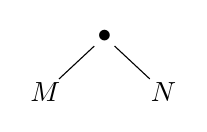
\begin{tikzpicture}[baseline=-3pt,level distance=7mm,
		every node/.style={inner sep=1pt}]
		\node {$\bullet$}
		child { node {$M$} }
		child { node {$N$} };
	\end{tikzpicture}
\]
This mapping is bijective between program terms (modulo $\alpha$-conversion) and
labeled elements of $\mathcal{C}$.

Pairs-expansions of combinators---for example the standard expansions of
$\mathrm{S}$ and $\mathrm{K}$ into $\lambda$-terms—produce larger trees but
remain within the Catalan family.  Thus the Catalan substrate is closed under
syntactic elaboration.

Operational semantics are likewise internal.  Both $\beta$-reduction and SKI
contraction replace subtrees with simpler subtrees while preserving the global
full-binary-tree form.  Each admissible reduction path therefore corresponds to
a trajectory within $\mathcal{C}$, and nondeterminism in reduction strategy
corresponds to branching structure within the Catalan tree itself.

This uniformity demonstrates that the Catalan substrate simultaneously captures:
\begin{enumerate}
	\item program syntax (binary application structure),
	\item program elaboration (via pairs-expansion or substitution), and
	\item program dynamics (via evaluation rewrites).
\end{enumerate}
Consequently, computation lives entirely within the Catalan family, justifying
its use as the structural substrate for the unified causal--computational model
developed in the main text.

\subsection{Illustrative Figures}

\begin{figure}[h]
	\centering
	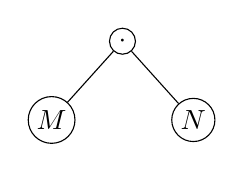
\begin{tikzpicture}[
		level distance=10mm,
		sibling distance=18mm,
		every node/.style={circle,draw,inner sep=1.5pt}
		]
		\node {$\cdot$}
			child { node {$M$} }
			child { node {$N$} };
	\end{tikzpicture}
	\caption{A binary application node representing the term $M\,N$.}
\end{figure}

\begin{figure}[h]
	\centering
	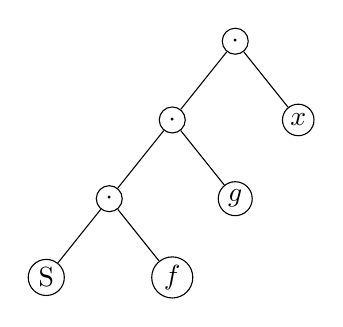
\begin{tikzpicture}[
		level distance=10mm,
		sibling distance=16mm,
		every node/.style={circle,draw,inner sep=1.5pt}
		]
		\node {$\cdot$}
			child {
				node {$\cdot$}
				child { node {$\cdot$} child { node {$\mathrm{S}$} } child { node {$f$} } }
				child { node {$g$} }
			}
			child { node {$x$} };
	\end{tikzpicture}
	\caption{Binary-tree representation of the term $\mathrm{S}\,f\,g\,x$.}
	\label{fig:Sfgx-binary-tree}
\end{figure}

\begin{figure}[h]
	\centering
	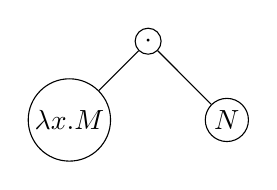
\begin{tikzpicture}[
		level distance=10mm,
		sibling distance=20mm,
		every node/.style={circle,draw,inner sep=1.5pt}
		]
		\node {$\cdot$}
			child { node {$\lambda x.M$} }
			child { node {$N$} };
	\end{tikzpicture}
	\qquad$\Longrightarrow$\qquad
	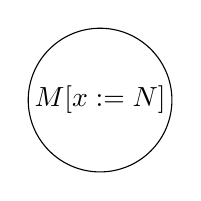
\begin{tikzpicture}[
		level distance=10mm,
		sibling distance=20mm,
		every node/.style={circle,draw,inner sep=1.5pt}
		]
		\node {$M[x:=N]$};
	\end{tikzpicture}
	\caption{$\beta$-reduction as a local rewrite inside the Catalan family.}
\end{figure}

\subsection{Pairs Expansion as Variable-Free S-Expressions}
\label{subsec:pairs-s-expressions}

A central observation motivating this work is that the pairs expansions of
combinators can be written as \emph{variable- and label-free} S-expressions,
exactly in the style of McCarthy's original Lisp notation \cite{McCarthy1960}.
In McCarthy's formulation, the core data structure is the cons-cell, written as
a parenthesized pair. Here we push this idea to an extreme: we erase all atom
labels and regard the program itself as a pure cons-tree, encoded only by
balanced parentheses.

Concretely, consider the binary application tree for the term
$\mathrm{S}\,f\,g\,x$ (as in Figure~\ref{fig:Sfgx-binary-tree}). Under the pairs
encoding used in our simulations, this same shape appears as the variable-free
S-expression
\[
	\texttt{(()(()(()())))}.
\]
This S-expression can also be understood as \emph{looking down into} the
underlying Catalan tree: the outer parentheses form the root frame, while each
\texttt{()} corresponds to a leaf. The corresponding unlabeled binary tree shape
is shown below.

\begin{center}
	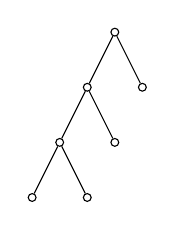
\begin{tikzpicture}[
		level 1/.style={level distance=7mm,sibling distance=7mm},
		level 2/.style={level distance=7mm,sibling distance=7mm},
		level 3/.style={level distance=7mm,sibling distance=7mm},
		every node/.style={circle,draw,inner sep=1pt,minimum size=2pt}
		]
		\node {}
			child { node {}
				child { node {}
					child { node {} }
					child { node {} }
				}
				child { node {} }
			}
			child { node {} };
	\end{tikzpicture}
\end{center}

Viewed from this perspective, the S-expression is simply the linear “parentheses
trace” of this structure: each ``('' corresponds to descending into a cons-cell,
each ``)'' corresponds to returning toward the trunk, and the empty pairs
\texttt{()} mark the terminal leaves.

More generally, the pairs bijection

\begin{small}
\begin{verbatim}
n=0, c=1:  ()
n=1, c=1:  (()())
n=2, c=2:  (()(()())) ((()())())
n=3, c=5:  (()(()(()()))) (()((()())())) ((()())(()())) ((()(()()))()) (((()())())())
\end{verbatim}
\end{small}

enumerates exactly the same Catalan shapes that appear as Dyck paths

\begin{verbatim}
n=1, c=1:  ()
n=2, c=2:  (()) ()()
n=3, c=5:  ((())) (()()) (())() ()(()) ()()()
\end{verbatim}

but seen through a different projection. The Dyck words present the
one-dimensional ``height'' profile of the walk, making the Lorentzian scaling
limit and the breadth--depth structure of the light cone transparent. The pairs
S-expressions, by contrast, foreground the \emph{binary computational
structure}: they are precisely the unlabeled S-expression trees of a Lisp-like
language, with cons as the sole constructor.
\footnote{Here “projection’’ is not a literal mapping but a change of
	coordinates on the same Catalan object. The Dyck, binary-tree, and
	S-expression representations are all related by canonical bijections; each is
	a different parametrization of the same underlying Catalan shape.  Thus
switching from Dyck words to pairs S-expressions does not change the object
itself, only the coordinate system through which it is viewed.}

In this sense, Dyck words and pairs expansions are two complementary Catalan
bijections:

\begin{itemize}
	\item Dyck words: a one-dimensional time--breadth profile well adapted to
		continuum limits and Lorentzian geometry;
	\item pairs S-expressions: a fully binary application tree well adapted to
		combinatory computation.
\end{itemize}

Both encode the same Catalan shapes; one may view them as distinct ``Lorentz
frames'' on the same underlying combinatorial substrate. The pairs expansion can
thus be regarded as an additional invariant transform: it preserves the Catalan
class while re-expressing the same light-cone structure in purely computational
coordinates.

There is also an intrinsic handedness in this picture. Dyck words of a given
semilength $n$ are not symmetric under reversal of the walk; the distribution of
shapes across the tier reflects the left-to-right order in which parentheses are
added. This asymmetry is the combinatorial trace of the fundamental handedness
of applicative collapse in the pairs expansion: application is not commutative,
and the collapse rule is oriented. The sequential construction of the
S-expression tree makes this visible as a bias in how breadth is accumulated
relative to depth.

A further simplification arises when we observe that in the S-expression view,
explicit application nodes disappear entirely. Application is seen as a
\emph{property of the parentheses themselves}: a nested pair structure is
already an applicative program. From the standpoint of Schönfinkel's combinatory
logic \cite{Schoenfinkel1924}, where even the familiar $\mathrm{S}$ and
$\mathrm{K}$ can be reduced to a single sufficiently expressive combinator, one
may heuristically say that if a lone combinator $J$ acting on parentheses is
enough, then we can omit $J$ and work directly with the bare parentheses~$()$.
The Catalan substrate then becomes a \emph{combinator-free} calculus of pure
application.

Traditional functional calculi admit multiple evaluation strategies
(normal-order, applicative-order, call-by-need, etc.). The Catalan substrate
makes explicit a natural causal preorder on redex positions (ancestor order),
constraining dependencies between contractions. Collapse is local, and
contractions supported on disjoint subtrees commute
(Lemma~\ref{lem:causal-consistency-long}). Different evaluation strategies may then
be viewed as different linearizations of the residual freedom to schedule
causally independent contractions (Appendix~\ref{appendix:computational-foundations}).

\paragraph{Historical Perspective.}

The S-expression viewpoint connects the present framework to three classical
constructions.  First, McCarthy's original Lisp treats cons-pairs as the sole
data constructor, with atoms added as a separate syntactic category
\cite{McCarthy1960}. Here we invert the hierarchy: structure is primary, and
atoms---if present at all---arise as designated structural motifs.

Second, Church encodings demonstrate that data and control structures can be
represented entirely by higher-order functions; similarly, SKI combinatory logic
eliminates variables altogether. These developments show that symbolic reference
is not primitive but can be reconstructed from purely structural or operational
primitives.

Third, Gödel numbering treats syntax as arithmetic structure. The present
approach may be viewed as a ``Catalan numbering,'' where syntactic entities are
mapped to unlabeled binary trees. The Dyck, pairs, and binary-tree bijections
then provide multiple coordinate systems for the same structural universe. In
this sense, the Catalan substrate acts simultaneously as a computational
calculus and as a structural semantics for symbolic systems.

\subsection{Symbolic Representation in a Structure-Only Substrate}
\label{subsec:symbolic-representation}

In the Catalan substrate all information is structural: the only primitive
constructor is the cons-pair, and there are no atomic labels. This raises a
fundamental question: how can a system without atoms support symbols, naming, or
reference? The answer is that symbols arise not as primitives but as
\emph{structural motifs} that function as internal or external markers depending
on context. We distinguish two forms of symbolic representation.

\subsubsection{Internal Structural Symbols}

Within a closed Catalan machine, one may bootstrap symbolic reference by
designating particular tree shapes as internal ``names.'' A higher-level
self-referential mechanism (conceptually similar to a Y-like fixed-point
operator) can maintain a dictionary of such shapes, mapping them to programs,
behaviours, or combinator expansions. In this mode, names are themselves Catalan
objects, and symbolic reference arises entirely from geometry: identifying a
symbol is equivalent to matching a structural pattern. This yields a Lisp-like
environment without atomic identifiers, where all ``atoms'' are implemented as
canonical shapes in the tree.

\subsubsection{External Structural Symbols}

When interacting with external systems, the same structural motifs can serve as
\emph{extrinsic} symbols. Distinguished shapes may encode character codes,
vector-drawing glyphs, device signals, or other forms of I/O. This does not
modify the underlying calculus: it merely overlays a conventional interpretation
on structural patterns. The Catalan substrate remains atomless internally, while
external systems treat designated shapes as meaningful codes.

\subsubsection{Unified View: Symbols as Distinguished Motifs}

Both internal and external naming mechanisms exemplify a common principle: in a
structure-only universe, symbols are not primitive entities but \emph{designated
Catalan motifs}. A symbol is simply a tree pattern endowed—internally or
externally—with stable semantic interpretation. The substrate itself does not
distinguish between data and code, or between program and identifier; all such
distinctions emerge from the placement and recognition of specific structural
forms.

\begin{definition}[Structural Symbol]

	A \emph{structural symbol} is a finite Catalan tree $S$ together with an
	interpretation map $\iota$ assigning $S$ either (i) an internal computational
	meaning within the Catalan machine, or (ii) an external semantic meaning
	communicated to an outside system. The substrate recognizes $S$ only as a
	structure; all semantics flow from~$\iota$.

\end{definition}

\begin{remark}

	Although traditional programming languages begin with atoms and build
	structure on top of them, the Catalan substrate inverts this perspective:
	structure comes first, and atoms (if needed) are reintroduced later as
	structural patterns. From this viewpoint Lisp's cons-based representation, and
	even Schönfinkel's proposal of a single universal combinator, appear naturally
	as degenerate cases of a more general structure-first semantics.

\end{remark}


\subsection{Causal Admissibility of Redex Contraction}
\label{subsec:causal-admissibility}

We now formalize the sense in which evaluation order is fixed by causality
rather than chosen by convention.

\begin{definition}[Causal Preorder on Positions]
	Let $T$ be a full binary tree in the Catalan substrate, representing a program
	term. A \emph{position} in $T$ is a node address $p$ in the usual tree sense
	(e.g.\ a finite word over $\{L,R\}$ indicating left/right choices from the
	root). We write $p \prec q$ if the node at position $p$ lies on the unique
	path from the root to the node at position $q$. The reflexive, transitive
	closure of $\prec$ defines a preorder $\preceq$ on positions, which we call
	the \emph{causal preorder}.
\end{definition}

Intuitively, $p \preceq q$ means that the subtree at $q$ is causally downstream of the subtree at $p$: any change at $p$ may propagate to $q$ but not conversely.

\begin{definition}[Redex and Causal Admissibility]
	A \emph{redex} in $T$ is a position $p$ such that the subtree rooted at $p$
	matches the left-hand side of a reduction rule (e.g.\ a $\beta$-redex or an
	SKI contraction). Let $R(T)$ be the set of all redex positions in $T$.

	A redex at position $p \in R(T)$ is \emph{causally admissible} if there is no
	other redex $q \in R(T)$ with $q \prec p$. In other words, a redex is causally
	admissible if it is minimal in $R(T)$ with respect to the strict causal order.
\end{definition}

\begin{definition}[Causally Admissible Reduction Sequence]
	A finite or infinite sequence of trees
	\[
		T_0 \to T_1 \to T_2 \to \cdots
	\]
	is \emph{causally admissible} if, for each step $T_i \to T_{i+1}$, the
	contracted redex is causally admissible in $T_i$ in the above sense. A
	\emph{causal computation} is a causally admissible sequence starting from some
	initial tree $T_0$.
\end{definition}


\begin{lemma}[Commutation of disjoint reductions]
	\label{lem:causal-consistency-long}
	Let $T$ be a Catalan tree (full binary tree) and let $p,q\in R(T)$ be two redex
	positions that are \emph{incomparable} under the causal preorder $\preceq$
	(i.e.\ neither lies on the path from the root to the other). Let $T_p$ denote
	the result of contracting the redex at $p$, and similarly $T_q$.
	Then $q$ remains a redex position in $T_p$ and $p$ remains a redex position in
	$T_q$, and contracting both redexes yields the same tree regardless of order:
	\[
		(T_p)_q \;\equiv\; (T_q)_p.
	\]
		In particular, disjoint reductions form a commuting diamond as in
		the usual commuting-diamond picture.
\end{lemma}

\begin{proof}[Proof sketch]
	Since $p$ and $q$ lie in disjoint subtrees, contracting at $p$ rewrites only
	the subtree rooted at $p$ and leaves the subtree rooted at $q$ unchanged. Thus
	the redex at $q$ is unaffected (and remains at the same position), so it may
	still be contracted in $T_p$. Symmetrically, contracting at $q$ leaves the
	subtree at $p$ unchanged. Because the two rewrite steps act on disjoint parts
	of the tree, performing both contractions yields the same result regardless of
	order.
\end{proof}


\subsection{Evaluation Strategies as Coarse-Grainings of Causal Order}
\label{subsec:evaluation-strategies}

Traditional presentations of the $\lambda$-calculus distinguish several
evaluation strategies: normal-order, applicative-order, call-by-need, and many
others. These are usually defined syntactically (e.g.\ by specifying which redex
is chosen at each step), with confluence guaranteeing that they terminate in the
same normal form when one exists. In the Catalan substrate, however, causality
constrains redex selection more tightly.

\begin{definition}[Strategy-Compatible Causal Computation]
	Let $\mathcal{S}$ be a syntactic evaluation strategy (e.g.\ normal-order or
	applicative-order) which, given a term, selects one or more redex positions
	considered ``eligible'' at each step. A causal computation
	\[
		T_0 \to T_1 \to \cdots
	\]
	is \emph{compatible} with $\mathcal{S}$ if, at each step, the contracted redex
	is both causally admissible in $T_i$ and belongs to the set of redexes
	selected by $\mathcal{S}$ for the corresponding term.
\end{definition}

\begin{proposition}[Strategies as Coarse-Grainings of Causal Structure]
	\label{prop:strategies-coarse-graining}
	Let $T_0$ be an initial term, and suppose $\mathcal{S}$ is a standard
	evaluation strategy that is normalizing on $T_0$ (e.g.\ normal-order for a
	weakly normalizing term). Then:
	\begin{enumerate}
		\item Every $\mathcal{S}$-guided reduction sequence can be refined to a
			causally admissible computation by reordering only reductions that occur
			at redexes incomparable under the causal preorder.
		\item Conversely, every causally admissible computation from $T_0$ to normal
			form projects to an $\mathcal{S}$-valid history by forgetting the precise
			interleaving of causally independent reductions.
	\end{enumerate}
	In this sense, classical evaluation strategies are coarse-grainings of the
	underlying causal order: they differ only in how they resolve the residual
	freedom to permute causally independent redex contractions.
\end{proposition}

\begin{proof}[Proof sketch]
	For (1), observe that any $\mathcal{S}$-guided sequence that temporarily
	contracts a non-minimal redex (with respect to $\preceq$) must do so in a
	context where all redexes on which it causally depends will eventually be
	contracted as well. By standard commuting-conversion arguments, we can reorder
	the sequence so that causally prior redexes are contracted first, without
	changing the final normal form. This reordering affects only redexes that lie
	in disjoint subtrees, i.e.\ are incomparable under $\preceq$.

	For (2), given a causally admissible computation, we can group together all
	contractions that $\mathcal{S}$ regards as taking place at the ``same'' redex
	position in the syntactic term, ignoring the precise ordering among
	contractions in disjoint subtrees. The resulting abstract history matches what
	$\mathcal{S}$ would produce, by confluence and the fact that $\mathcal{S}$ is
	normalizing on $T_0$. Thus $\mathcal{S}$ may be seen as a projection that
	forgets the fine-grained causal structure of independent collapses while
	preserving the global reduction behaviour.
	\end{proof}

\fi



		\bibliographystyle{plain}
		\begin{thebibliography}{99}

	\bibitem{addario-berry13}
	L.~Addario-Berry, L.~Devroye, and S.~Janson.
	\newblock Sub-Gaussian tail bounds for the width and height of conditioned
	Galton--Watson trees.
	\newblock {\em Annals of Probability}, 41(2):1074--1087, 2013.

	\bibitem{ambjorn01}
	J.~Ambj{\o}rn, J.~Jurkiewicz, and R.~Loll.
	\newblock Dynamically triangulating Lorentzian quantum gravity.
	\newblock {\em Nuclear Physics B}, 610:347--382, 2001.

	\bibitem{ambjorn12}
	J.~Ambj{\o}rn, A.~G{\"o}rlich, J.~Jurkiewicz, and R.~Loll.
	\newblock Nonperturbative quantum gravity.
	\newblock {\em Physics Reports}, 519:127--210, 2012.

	\bibitem{barendregt84}
	H.~P. Barendregt.
	\newblock {\em The Lambda Calculus: Its Syntax and Semantics}.
	\newblock North-Holland, 1984.

	\bibitem{bombelli87}
	L.~Bombelli, J.~Lee, D.~Meyer, and R.~D. Sorkin.
	\newblock Space-time as a causal set.
	\newblock {\em Physical Review Letters}, 59(5):521--524, 1987.

	\bibitem{church33}
	A.~Church.
	\newblock A set of postulates for the foundation of logic.
	\newblock {\em Annals of Mathematics}, 34:839--864, 1933.

	\bibitem{McCarthy1960}
	J.~McCarthy.
	\newblock Recursive functions of symbolic expressions and their computation by
	machine, Part~I.
	\newblock {\em Communications of the ACM}, 3(4):184--195, 1960.

		\bibitem{CurryFeys1958}
		H.~B. Curry and R.~Feys.
		\newblock {\em Combinatory Logic, Vol.~I}.
		\newblock North-Holland, 1958.

	\bibitem{feynman-hibbs65}
	R.~P. Feynman and A.~R. Hibbs.
	\newblock {\em Quantum Mechanics and Path Integrals}.
	\newblock McGraw--Hill, 1965. (Dover reprint, 2010).

	\bibitem{janson07}
	S.~Janson.
	\newblock Brownian excursion area, Wright's constants in graph enumeration, and
	other Brownian areas.
	\newblock {\em Probability Surveys}, 4:80--145, 2007.

	\bibitem{kac49}
	M.~Kac.
	\newblock On distributions of certain Wiener functionals.
	\newblock {\em Transactions of the American Mathematical Society},
	65(1):1--13, 1949.

	\bibitem{le-gall05}
	J.-F. Le~Gall.
	\newblock Random trees and applications.
	\newblock {\em Probability Surveys}, 2:245--311, 2005.

		\bibitem{orus14}
		R.~Or\'us.
			\newblock A practical introduction to tensor networks: Matrix product states and
			projected entangled pair states.
			\newblock {\em Annals of Physics}, 349:117--158, 2014.

		\bibitem{pitman1999}
		J.~Pitman.
		\newblock Brownian motion, bridge, excursion, and meander revisited.
		\newblock {\em Electronic Journal of Probability}, 4:1--32, 1999.

		\bibitem{Schoenfinkel1924}
		M.~Sch{\"o}nfinkel.
		\newblock {\"U}ber die Bausteine der mathematischen Logik.
		\newblock {\em Mathematische Annalen}, 92:305--316, 1924.

		\bibitem{rovelli04}
		C.~Rovelli.
		\newblock {\em Quantum Gravity}.
		\newblock Cambridge University Press, 2004.

			\bibitem{stanley-catalan}
			R.~P. Stanley.
			\newblock {\em Catalan Numbers}.
			\newblock Cambridge University Press, 2015.

		\bibitem{takacs1991}
		L.~Tak{\'a}cs.
		\newblock A {B}ernoulli excursion and its various applications.
		\newblock {\em Advances in Applied Probability}, 23(3):557--585, 1991.

		\bibitem{cheneviere2022linear}
		C.~Chenevi\`ere.
		\newblock Linear intervals in the Tamari and the Dyck lattices and in the
		alt-Tamari posets.
		\newblock arXiv:2209.00418v2, 2022.

	\bibitem{abhy2018scatteringforms}
	N.~Arkani-Hamed, Y.~Bai, S.~He, and G.~Yan.
	\newblock Scattering forms and the positive geometry of kinematics, color and
	the worldsheet.
	\newblock {\em JHEP} \textbf{05} (2018) 096.
	\newblock arXiv:1711.09102.

	\bibitem{banerjee2018stokes}
	P.~Banerjee, A.~Laddha, and P.~Raman.
	\newblock Stokes polytopes: The positive geometry for $\phi^4$ interactions.
	\newblock arXiv:1811.05904, 2018.

	\bibitem{herrmann2022positivegeometry}
	E.~Herrmann and J.~Trnka.
	\newblock Positive geometry of scattering amplitudes.
	\newblock arXiv:2203.13018, 2022.

	\end{thebibliography}
\end{document}
